\documentclass{article}\usepackage[]{graphicx}\usepackage[]{xcolor}
% maxwidth is the original width if it is less than linewidth
% otherwise use linewidth (to make sure the graphics do not exceed the margin)
\makeatletter
\def\maxwidth{ %
  \ifdim\Gin@nat@width>\linewidth
    \linewidth
  \else
    \Gin@nat@width
  \fi
}
\makeatother

\definecolor{fgcolor}{rgb}{0.345, 0.345, 0.345}
\newcommand{\hlnum}[1]{\textcolor[rgb]{0.686,0.059,0.569}{#1}}%
\newcommand{\hlstr}[1]{\textcolor[rgb]{0.192,0.494,0.8}{#1}}%
\newcommand{\hlcom}[1]{\textcolor[rgb]{0.678,0.584,0.686}{\textit{#1}}}%
\newcommand{\hlopt}[1]{\textcolor[rgb]{0,0,0}{#1}}%
\newcommand{\hlstd}[1]{\textcolor[rgb]{0.345,0.345,0.345}{#1}}%
\newcommand{\hlkwa}[1]{\textcolor[rgb]{0.161,0.373,0.58}{\textbf{#1}}}%
\newcommand{\hlkwb}[1]{\textcolor[rgb]{0.69,0.353,0.396}{#1}}%
\newcommand{\hlkwc}[1]{\textcolor[rgb]{0.333,0.667,0.333}{#1}}%
\newcommand{\hlkwd}[1]{\textcolor[rgb]{0.737,0.353,0.396}{\textbf{#1}}}%
\let\hlipl\hlkwb

\usepackage{framed}
\makeatletter
\newenvironment{kframe}{%
 \def\at@end@of@kframe{}%
 \ifinner\ifhmode%
  \def\at@end@of@kframe{\end{minipage}}%
  \begin{minipage}{\columnwidth}%
 \fi\fi%
 \def\FrameCommand##1{\hskip\@totalleftmargin \hskip-\fboxsep
 \colorbox{shadecolor}{##1}\hskip-\fboxsep
     % There is no \\@totalrightmargin, so:
     \hskip-\linewidth \hskip-\@totalleftmargin \hskip\columnwidth}%
 \MakeFramed {\advance\hsize-\width
   \@totalleftmargin\z@ \linewidth\hsize
   \@setminipage}}%
 {\par\unskip\endMakeFramed%
 \at@end@of@kframe}
\makeatother

\definecolor{shadecolor}{rgb}{.97, .97, .97}
\definecolor{messagecolor}{rgb}{0, 0, 0}
\definecolor{warningcolor}{rgb}{1, 0, 1}
\definecolor{errorcolor}{rgb}{1, 0, 0}
\newenvironment{knitrout}{}{} % an empty environment to be redefined in TeX

\usepackage{alltt}
\usepackage{wrapfig}
\usepackage[bottom=1in,top=1in,right=0.5in,left=0.5in]{geometry}
\usepackage{amsfonts}
\usepackage{fancyvrb}
\usepackage{amsmath}
\usepackage{multicol}
\usepackage{amssymb}
\usepackage{enumitem}
\usepackage{xfrac}
\usepackage[colorlinks=true, linkcolor=red]{hyperref}
\usepackage[nameinlink]{cleveref}
\crefformat{section}{\S#2#1#3}
\crefmultiformat{section}{\S\S#2#1#3}{ and~#2#1#3}{, #2#1#3}{, and~#2#1#3}
\crefformat{paragraph}{\S#2#1#3}
\crefmultiformat{paragraph}{\S\S#2#1#3}{ and~#2#1#3}{, #2#1#3}{, and~#2#1#3}
\crefformat{subparagraph}{\S#2#1#3}
\crefmultiformat{subparagraph}{\S\S#2#1#3}{ and~#2#1#3}{, #2#1#3}{, and~#2#1#3}
\crefformat{subsubparagraph}{\S#2#1#3}
\crefmultiformat{subsubparagraph}{\S\S#2#1#3}{ and~#2#1#3}{, #2#1#3}{, and~#2#1#3}
\setlist{noitemsep}
\title{Workshop calculations}
\IfFileExists{upquote.sty}{\usepackage{upquote}}{}
\begin{document}
\maketitle
\tableofcontents
 
\setlist{nosep}






%%%%%%%%%%%%%%%%%%%%%%%%%%%%%%%%%%%%%%%%%%%%%%%%%%%%%%%%%%%%%%%%%%%%%%%%%%%%%%%%

\section*{Notes}

\begin{itemize}
  \item In ``Imported variables'' we don't include those which just get the imperial string for variables defined elsewhere. These aren't important enough to count as genuine imported variables. 
  \item There should be \textbf{no} variables for mortise thickness, only tenon thickness. This is to prevent inadvertent differing definitions of tenon and mortise thicknesses. When the time to cut comes, use the slick to shave off tenon depth until we get a tight fit. 
\end{itemize}




\section{Ridge shape and dimensions} \label{ridge-shape-and-dimensions}


\subsection{Assumptions} \label{ridge-shape-and-dimensions-assumptions}

\begin{knitrout}
\definecolor{shadecolor}{rgb}{0.969, 0.969, 0.969}\color{fgcolor}\begin{kframe}
\begin{alltt}
\hlstd{rise} \hlkwb{<-} \hlnum{10}
\hlstd{run} \hlkwb{<-} \hlnum{12}
\hlstd{theta} \hlkwb{<-} \hlkwd{atan}\hlstd{(rise}\hlopt{/}\hlstd{run)}
\hlstd{theta_degrees} \hlkwb{<-} \hlkwd{rads_to_degs}\hlstd{(theta)}
\hlstd{theta1} \hlkwb{<-} \hlkwd{atan}\hlstd{(run}\hlopt{/}\hlstd{rise)}
\hlstd{theta1_degrees} \hlkwb{<-} \hlkwd{rads_to_degs}\hlstd{(theta1)}

\hlstd{purlin_height} \hlkwb{<-} \hlnum{7}
\hlstd{purlin_pocket} \hlkwb{<-} \hlnum{1}
\hlstd{purlin_height_above_rafter} \hlkwb{<-} \hlstd{purlin_height} \hlopt{-} \hlstd{purlin_pocket}

\hlstd{kp_width} \hlkwb{<-} \hlnum{8} \hlcom{# at the top}
\hlstd{ridge_width} \hlkwb{<-} \hlstd{kp_width}
\hlstd{kp_part} \hlkwb{<-} \hlnum{4.5} \hlcom{# straight part above rafters}
\end{alltt}
\end{kframe}
\end{knitrout}

\subsection{Imported variables} \label{ridge-shape-and-dimensions-imported-variables}

\begin{itemize}
  \item None. 
\end{itemize}

\subsection{Calculations} \label{ridge-shape-and-dimensions-calculations}
\begin{center}
	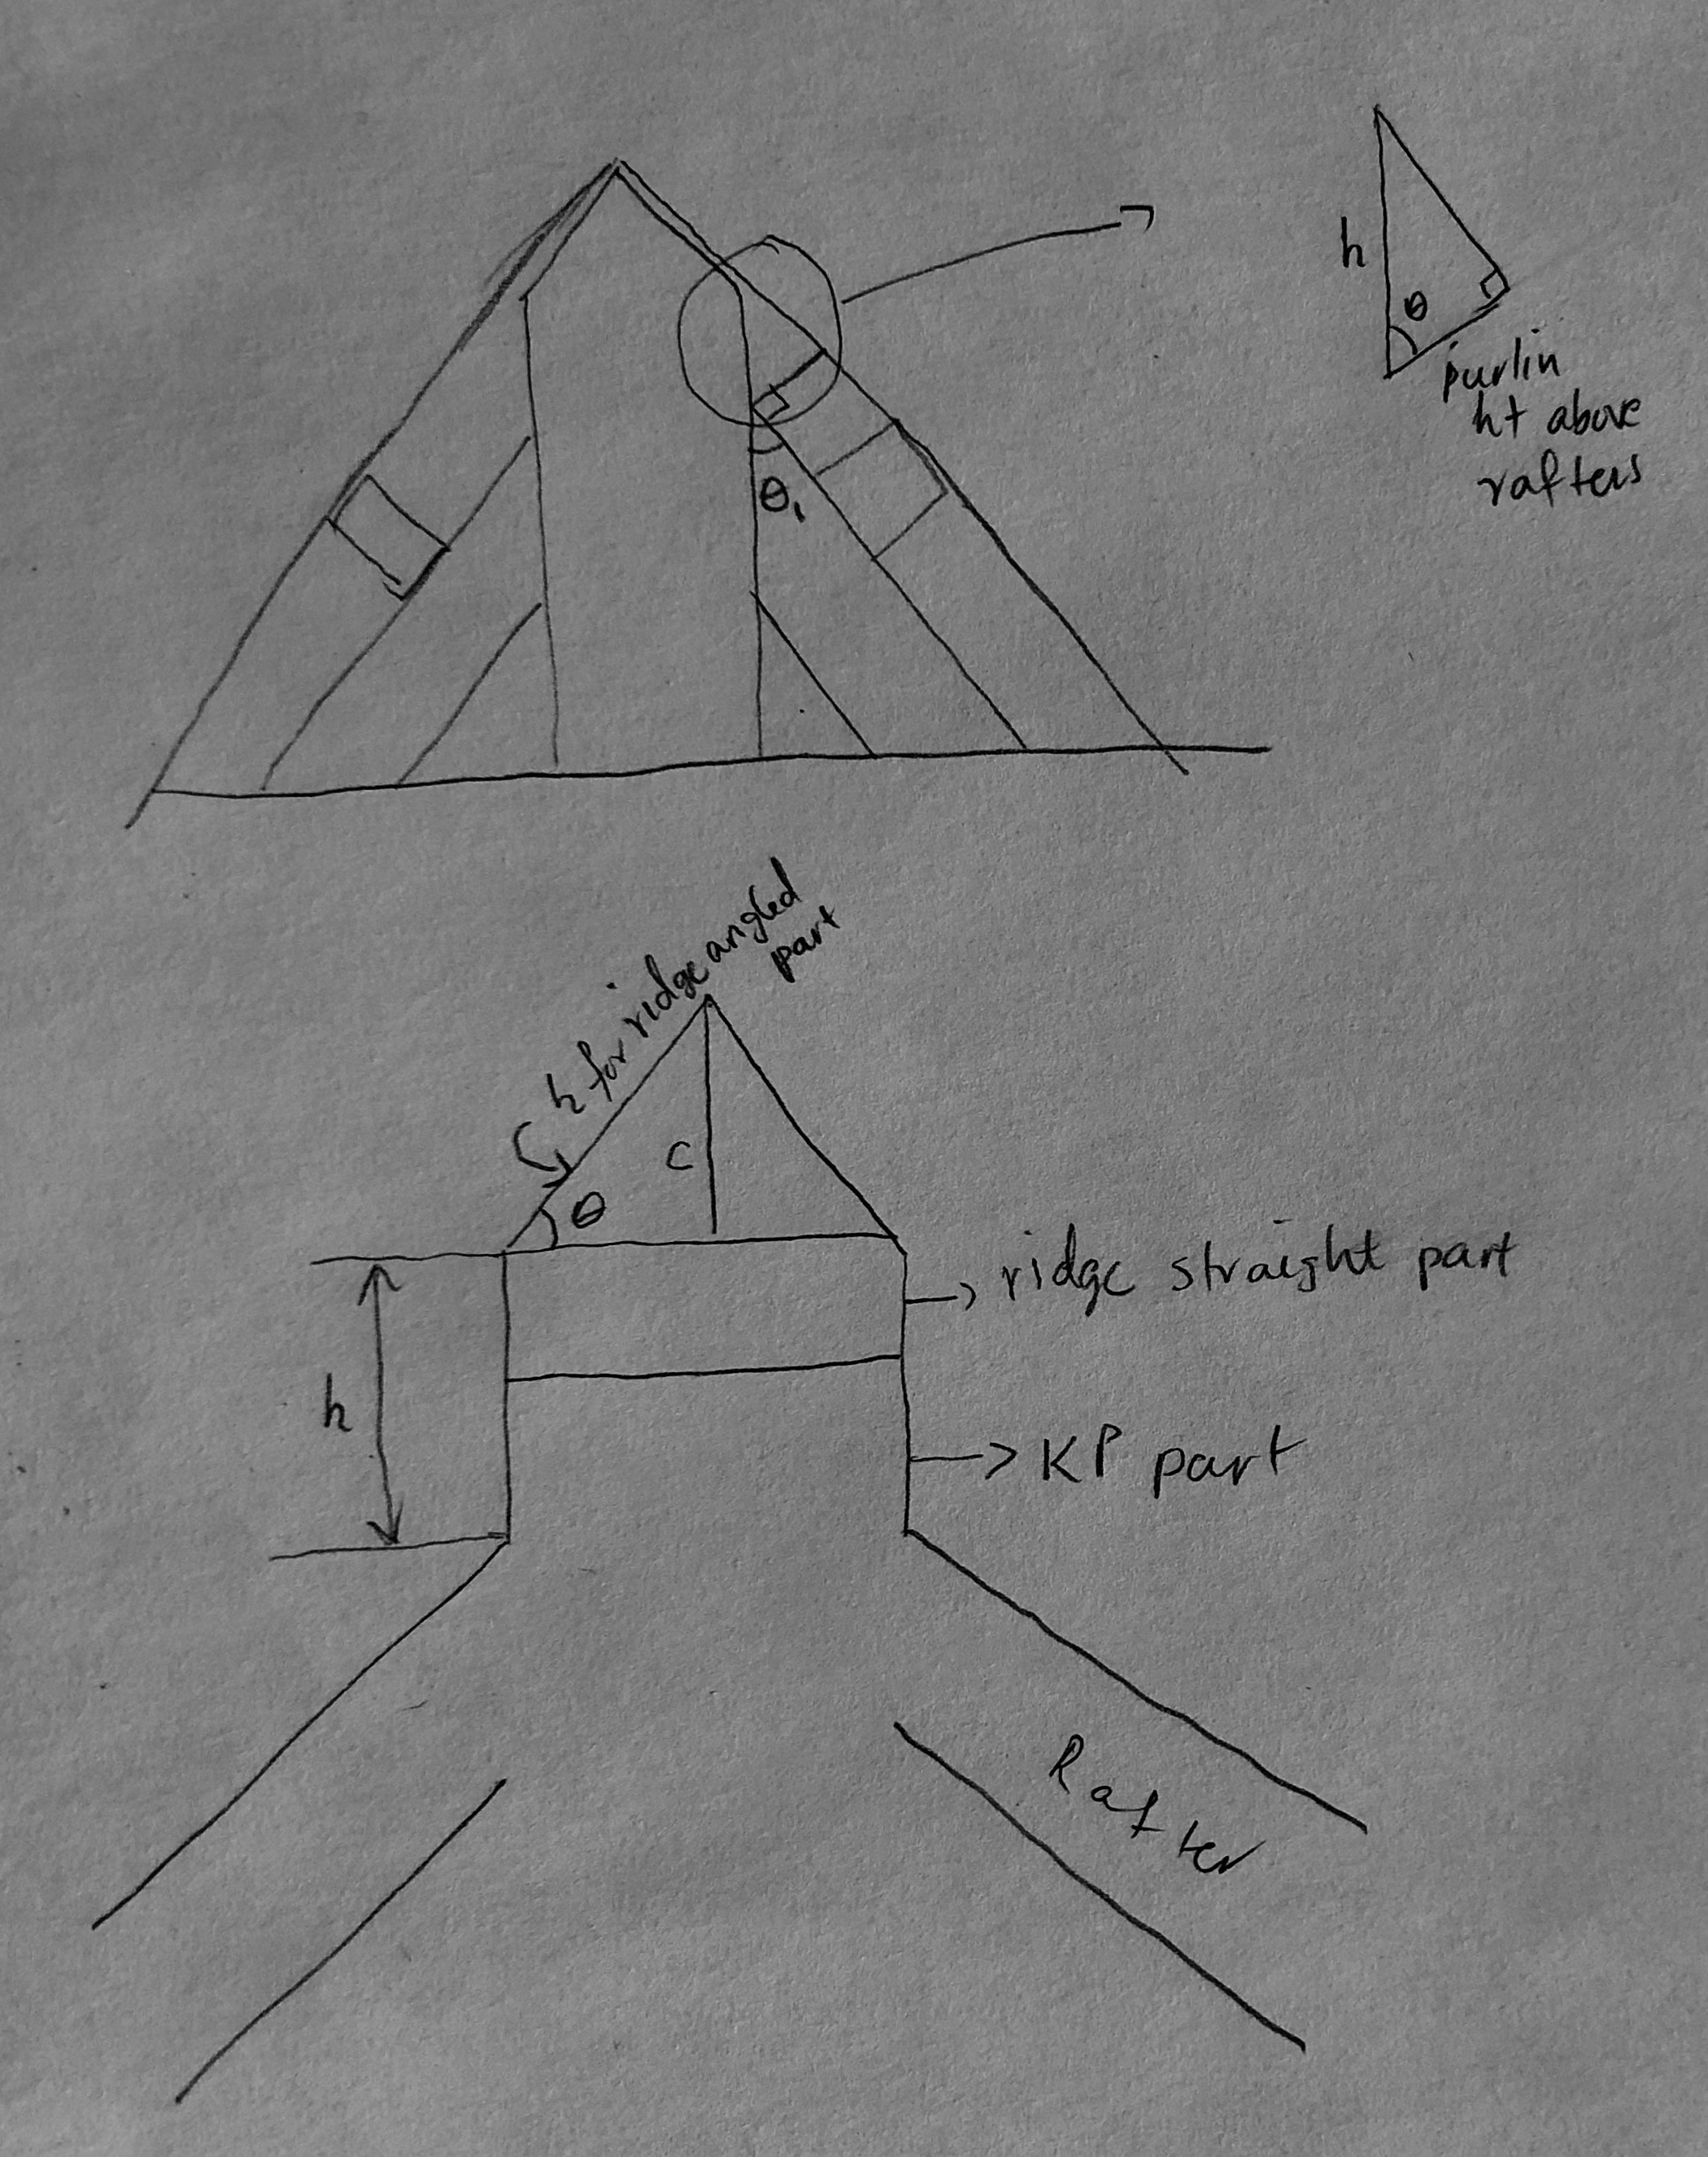
\includegraphics[width=0.35\textwidth]{images/ridge_calculations}
\end{center}


Start by knowing only roof pitch and purlin height above rafters. These determine the value of $h$ in the diagram: 
\[ h = 7.8102.\]

We set KP part to a reasonable amount (cf \Cref{ridge-shape-and-dimensions-assumptions}), and this dictates that
\[ \text{ridge straight part} = 3.3102.\]

The height for ridge angled part is dictated by roof pitch and ridge width: 
\[c = 3.3333\]
which means that
\[  \boxed{\text{Ridge total height} = 6.6436 = \text{0' 6" 21/32}} \]
and this is the milling height for this beam. Finally, ridge cross-sectional area = 39.8153, volume = 5733.4076, which in board feet is 39.8153. Divide cross-sectional area by beam width to find ``equivalent'' height. We find that this pentagonal beam is equivalent to a 8$\times$4.9769 beam for the purposes of $F_b$ calculations.





%%%%%%%%%%%%%%%%%%%%%%%%%%%%%%%%%%%%%%%%%%%%%%%%%%%%%%%%%%%%%%%%%%%%%%%%%%%%%%%%



\section{Kingpost length and and collar tie rough length}\label{kp-and-collar-tie-lengths}

\subsection{Assumptions} \label{kp-collar-tie-assumptions}


\begin{knitrout}
\definecolor{shadecolor}{rgb}{0.969, 0.969, 0.969}\color{fgcolor}\begin{kframe}
\begin{alltt}
\hlstd{structure_width} \hlkwb{<-} \hlnum{15}\hlopt{*}\hlnum{12}
\hlstd{structure_height} \hlkwb{<-} \hlnum{15}\hlopt{*}\hlnum{12}
\hlstd{structure_width_half} \hlkwb{<-} \hlstd{structure_width}\hlopt{/}\hlnum{2}
\hlstd{post_width} \hlkwb{<-} \hlnum{8}
\hlstd{rafter_height} \hlkwb{<-} \hlnum{8}
\hlstd{collar_tie_height} \hlkwb{<-} \hlnum{8}
\hlstd{kp_through_tenon_length} \hlkwb{<-} \hlnum{2}
\hlstd{kp_top_tenon_length} \hlkwb{<-} \hlnum{3}
\hlstd{dpct} \hlkwb{<-} \hlnum{5.853} \hlcom{# distance along rafter between post and collar tie}
\hlstd{overhang_sides} \hlkwb{<-} \hlnum{24} \hlcom{# inches}
\end{alltt}
\end{kframe}
\end{knitrout}
We start with purlin height above rafters, and the width of the structure. Ignore collar tie for now.

\subsection{Imported variables} \label{kp-collar-tie-imported-variables}

\begin{itemize}
  \item \verb+kp_width+ = 8 from \Cref{ridge-shape-and-dimensions-assumptions}.
  \item \verb+purlin_height_above_rafter+ = 6 from \Cref{ridge-shape-and-dimensions-assumptions}.
  \item \verb+kp_part+ = 4.5 from \Cref{ridge-shape-and-dimensions-assumptions}.
\end{itemize}

\subsection{Calculations} \label{kp-collar-tie-calculations}




\begin{center}
	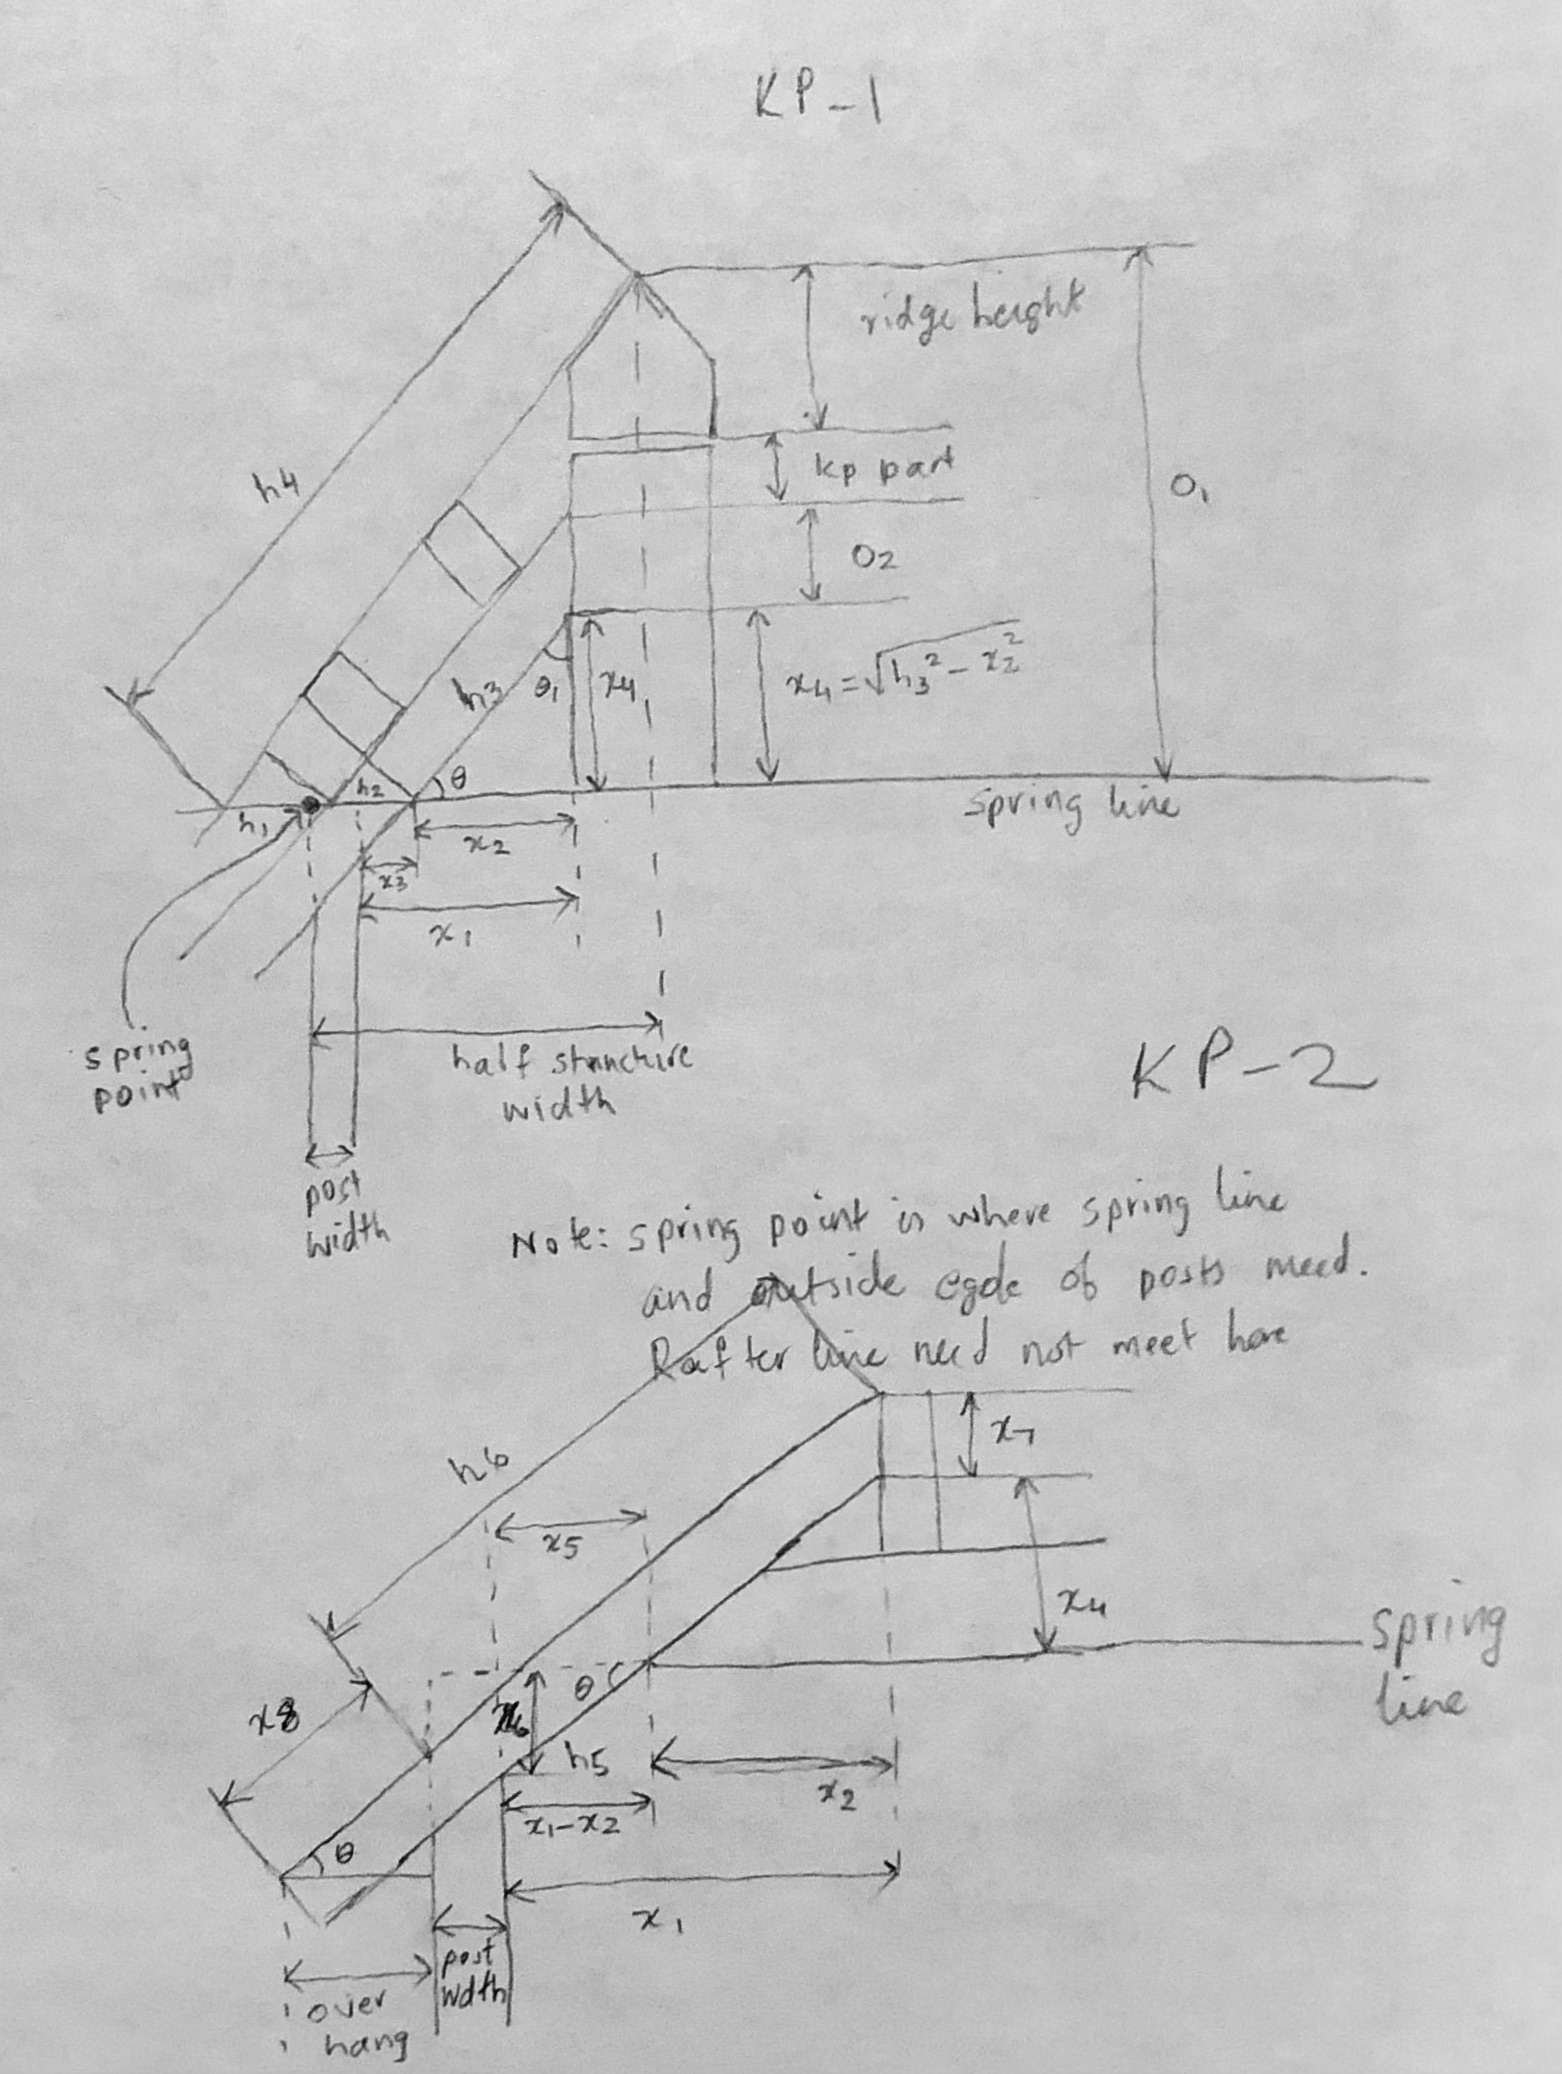
\includegraphics[width=0.55\textwidth]{images/kingpost_and_collar_tie_lengths}
\end{center}

\begin{align*}
x_1 &= \sfrac{1}{2} \text{ structure width} - \text{post width} - \sfrac{1}{2} \text{ kingpost width} = 78\\
o_2 &= \text{rafter height}/\sin\theta_1 = 10.4137\\
h_2 &= \text{rafter height}/\sin\theta = 12.4964\\
x_3 &= x_1 - x_2 = 4.4964\\
x_2 &= \sfrac{1}{2} \text{ structure width} - \sfrac{1}{2}\text{ kingpost width} - a_8 = 73.5036\\
h_3 &= x_2/\cos\theta = 95.6802\\
x_4 &= \tan\theta \times x_2  = 61.253
\end{align*}

Using $x_4$ from above, KP from top (excluding tenon) to spring line is 
\begin{align*}
\text{kp part (cf \Cref{ridge-shape-and-dimensions-assumptions}) } + o_2 + x_4 &= 76.1667\\
& = \text{6' 4" 5/32}
\end{align*}

We can also calculate for later:
\begin{align*}
h_1 &= \text{purlin height above rafters}/\sin\theta = 9.3723\\
h_4 &= a_1/\sin\theta  = 117.1537\\
o_1 &=  c + \text{ridge part} + \text{kp part} + o_2 + x_4 = 82.8102
\end{align*}

Calculating $o_1$ a different way: add up ridge height, kp part, $o_2$, and $x_4$, to get 82.8102, which should match the above. 

Since KP from top (excluding tenon) to spring line is 76.1667, and bottom of collar tie is at the spring line, KP length excluding \textbf{both} tenons is 76.1667 - 8 (collar tie height) = 68.1667. Assuming a 2-inch through tenon at bottom and 3-inch tenon at the top, we have 

\[ \boxed{\text{KP length }= 68.1667 + 8 + 2 + 3 = 81.1667 =  \text{6' 9" 5/32}}.\]

\textbf{Roughly}, collar tie length, assuming 5-inch tenons, is $x_2\times 2 + \text{KP width} + \text{tenon lengths} = $ 165.0072. See \Cref{collar-tie-final-length} for more accurate calculations.




%%%%%%%%%%%%%%%%%%%%%%%%%%%%%%%%%%%%%%%%%%%%%%%%%%%%%%%%%%%%%%%%%%%%%%%%%%%%%%%%




\section{Post length excluding tenons and rough rafter length}\label{posts-and-rafters}


\subsection{Assumptions}\label{posts-rafters-assumptions}
\begin{knitrout}
\definecolor{shadecolor}{rgb}{0.969, 0.969, 0.969}\color{fgcolor}\begin{kframe}
\begin{alltt}
\hlstd{structure_height} \hlkwb{<-} \hlnum{15}\hlopt{*}\hlnum{12} \hlcom{# top of ridge to base}
\hlstd{rafter_tenons_preliminary} \hlkwb{<-} \hlnum{3} \hlcom{# assuming 3 inch tenons; to be made precise later}
\end{alltt}
\end{kframe}
\end{knitrout}


\subsection{Imported variables} \label{posts-rafters-imported-variables}
\begin{itemize}
  \item $h_5$ from \Cref{kp-collar-tie-calculations}.
  \item $x_5$ from \Cref{kp-collar-tie-calculations}.
  \item ``top of ridge to spring line'' is ``kp height to spring line excl top tenon'' from \Cref{kp-collar-tie-calculations} and ``ridge height'' from \Cref{ridge-shape-and-dimensions-calculations}.
  \item Post width is from \Cref{kp-collar-tie-assumptions}.
  \item $x_1$ is from \Cref{kp-collar-tie-calculations}.
\end{itemize}


\subsection{Calculations} \label{posts-rafters-calculations}

\begin{center}
  \fbox{The diagram for this section is in the previous section.}
\end{center}



\[ x_6 = \tan\theta\times x_5 = 3.747. \]

From base to spring line is 
\begin{align*}
\text{structure height - (top of ridge to spring line)} &= 180 - 82.8102\\
&= 97.1898\\
&= \text{8' 1" 3/16}
\end{align*}

Post height excluding tenons is 
\[ 97.1898 - 3.747 = 93.4428 = \text{7' 9" 7/16}  \]

$x_8$ depends on overhang: 
\[ x_8 = \frac{\text{overhang}}{\cos\theta} = 31.241. \]

Also, 
\[ h_6 = \frac{\text{post width + }x_1}{\cos\theta} = 111.9469 \]

So \textbf{rough} rafter length, assuming 3-inch tenons is 
\[ x_8 + h_6 + 3 = 146.1879 = \text{12' 2" 3/16}.\]

See \Cref{kp-rafter-joints-calculations} for more precise measurements.




%%%%%%%%%%%%%%%%%%%%%%%%%%%%%%%%%%%%%%%%%%%%%%%%%%%%%%%%%%%%%%%%%%%%%%%%%%%%%%%%






\section{Kingpost/rafter joints and rafter final length}\label{kingpost-rafter-joints}

\subsection{Assumptions}  \label{kp-rafter-joints-assumptions}

\begin{knitrout}
\definecolor{shadecolor}{rgb}{0.969, 0.969, 0.969}\color{fgcolor}\begin{kframe}
\begin{alltt}
\hlstd{kp_rafter_shoulder_depth} \hlkwb{<-} \hlnum{1} \hlcom{# along the x axis}
\hlstd{rafter_tenon_depth_into_kp} \hlkwb{<-} \hlnum{3} \hlcom{# along the x axis}
\hlstd{rafter_tenon_thickness} \hlkwb{<-} \hlnum{2}
\hlcom{# In this section assume no KP flare}
\end{alltt}
\end{kframe}
\end{knitrout}



\subsection{Imported variables} \label{kp-rafter-joints-imported-variables}
\begin{itemize}
  \item \verb+kp_top_tenon_length+ = 3 from \Cref{kp-collar-tie-assumptions}. Here \verb+k_1+.
  \item \verb+kp_part+ = 4.5 from \Cref{ridge-shape-and-dimensions-assumptions}.
  \item \verb+rafter_height+ = 8 from \Cref{kp-collar-tie-assumptions}. 
  \item \verb+collar_tie_height+ = 8 from \Cref{kp-collar-tie-assumptions}.
  \item \verb+kp_through_tenon_length+ = 2 from \Cref{kp-collar-tie-assumptions}
  \item \verb+kp_total_height+ = 81.1667 from \Cref{kp-collar-tie-calculations}
  \item \verb+x8+ = 31.241 from \Cref{posts-rafters-calculations}
  \item \verb+h6+ from 111.9469 from \Cref{posts-rafters-calculations}
\end{itemize}



\subsection{Calculations} \label{kp-rafter-joints-calculations}

\begin{center}
\fbox{Ignore anything in these diagrams following that isn't relevant, like hardcoded values.}
\end{center}

\begin{center}
	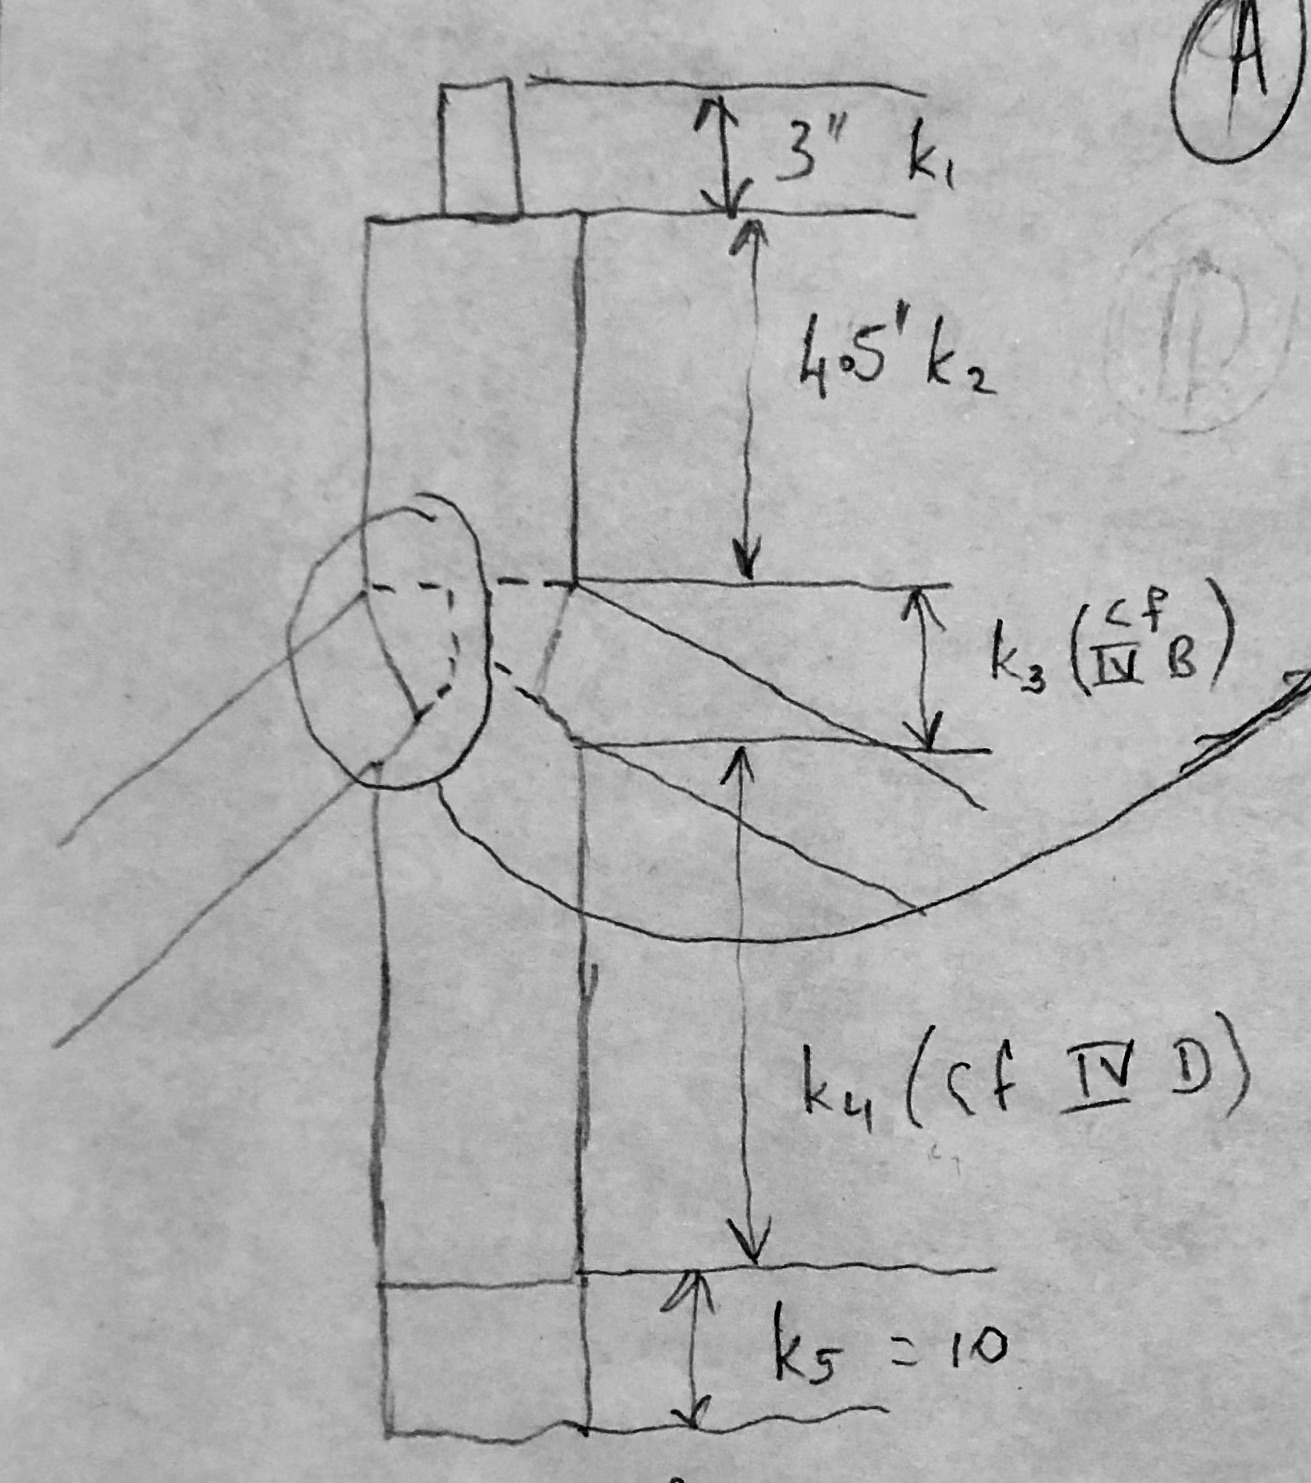
\includegraphics[width=0.4\textwidth]{images/kingpost_overall}
\end{center}





The variable for ``KP part'' was not labeled in \Cref{ridge-shape-and-dimensions-assumptions}; here we label it as $k_2$; its value is 4.5. The KP tenon height into ridge ($k_1$) is 3 (cf \Cref{kp-rafter-joints-imported-variables}). The variable $k_3$ is just rafter height divided by the cosine, which is 
\[ k_3 = \text{rafter height}/\cos\theta = 10.4137.   \]

\begin{center}
	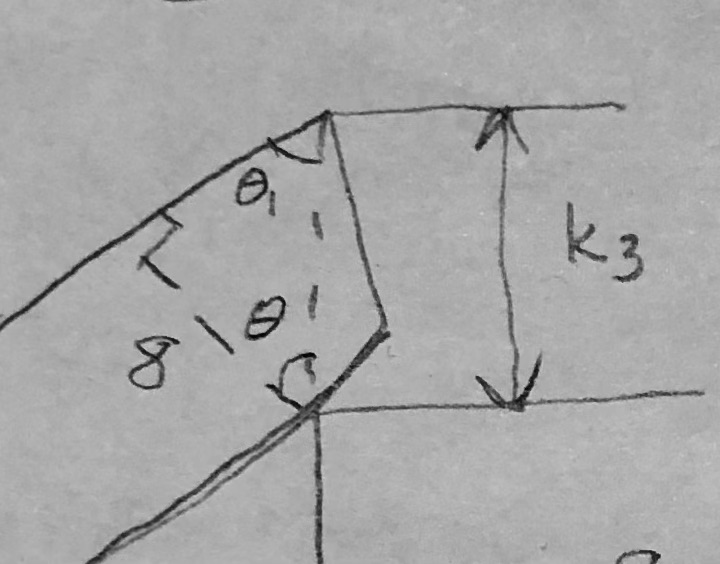
\includegraphics[width=0.3\textwidth]{images/k3}
\end{center}

The variable $k_5$ is given by collar tie height + through tenon length; here we have $k_5 = 10$. Then we have 
\[ k_4 = \text{KP total length} - k_1 - k_2 - k_3 - k_5 = 53.253. \]


\begin{center}
	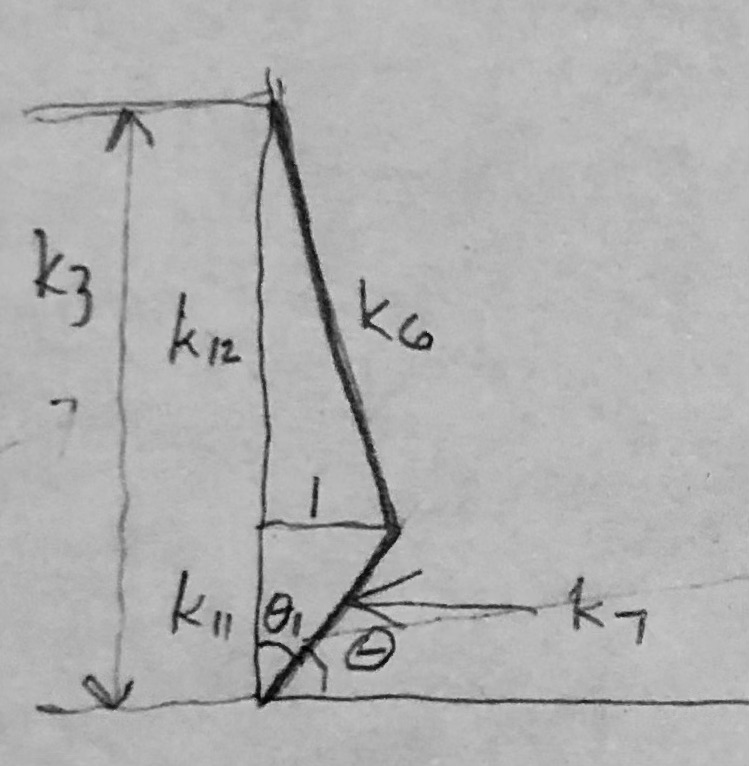
\includegraphics[width=0.4\textwidth]{images/kp_shoulder_angles}
\end{center}


The variables defined around the rafter-to-kp-shoulder are 
\begin{align*}
k_7 &= 1.3017\\
k_{11} &= 0.8333\\
k_{12} &= 9.5803\\
k_6 &= 9.6324
\end{align*}

\begin{center}
	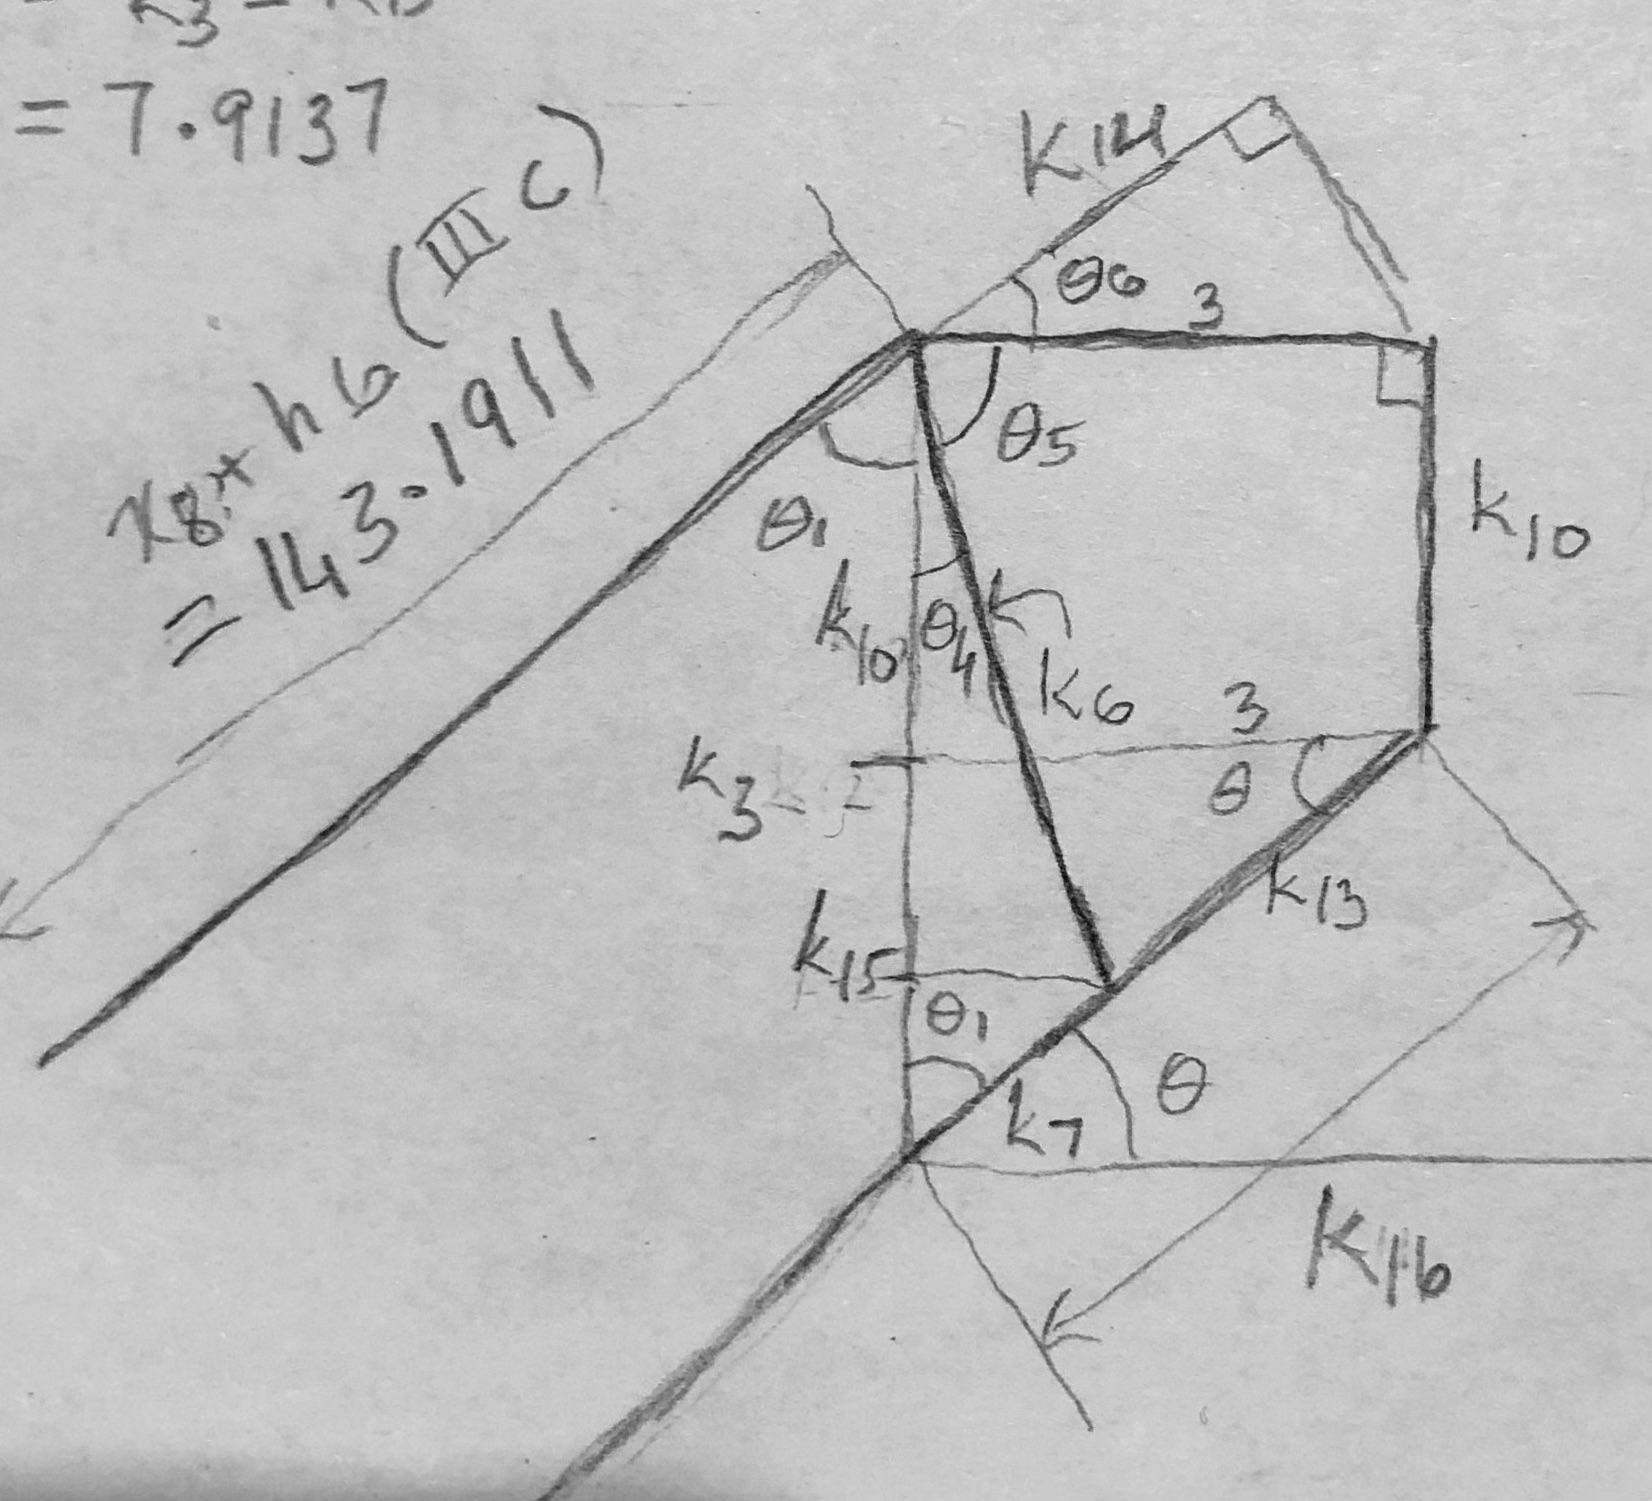
\includegraphics[width=0.45\textwidth]{images/rafter_tenon_detail}
\end{center}

The variables around rafter tenon/shoulder\footnote{It would seem that variable names $k_8$ and $k_9$ were never used in the paper drawings.} are 
\begin{align*}
k_{16} &= \text{rafter tenon depth into KP}/\cos\theta = 3.9051\\
k_{13} &= k_{16} - k_7 = 2.6034\\
\theta_4 &= \arccos \left(\frac{k_{12}}{k_6}\right) = 5.959\\
\theta_5 &= 90 - \theta_4 = 84.041\\
\theta_6 &= 180 - \theta_1 - \theta_4 - \theta_5 = 39.8056\\
k_{14} &= \text{rafter tenon depth into KP} \times \cos\theta_6 = 2.3047\\
k_{15} &= k_{16} \times \sin\theta = 2.5\\
k_{10} &= k_3 - k_{15} = 7.9137
\end{align*}



Now, we can calculate rafter length more precisely than in \Cref{posts-rafters-calculations}, where we just estimated the tenon length. We have 

\[ \boxed{\text{Rafter length} = x_8 + h_6 + k_{14} = 145.4926 = \text{12' 1" 1/2}.}\]

 






%%%%%%%%%%%%%%%%%%%%%%%%%%%%%%%%%%%%%%%%%%%%%%%%%%%%%%%%%%%%%%%%%%%%%%%%%%%%%%%%


 




\section{Rafter connections} \label{rafter-lengths-and-connections}

\subsection{Assumptions} \label{rafter-lengths-connections-assumptions}
\begin{knitrout}
\definecolor{shadecolor}{rgb}{0.969, 0.969, 0.969}\color{fgcolor}\begin{kframe}
\begin{alltt}
\hlstd{post_tenon_depth_into_rafter} \hlkwb{<-} \hlnum{4}
\hlstd{post_rafter_shoulder_depth} \hlkwb{<-} \hlnum{1}
\hlstd{collar_tie_rafter_shoulder_depth} \hlkwb{<-} \hlnum{1}
\hlstd{collar_tie_tenon_into_rafter_thickness} \hlkwb{<-} \hlnum{2}
\hlstd{collar_tie_tenon_into_rafter_depth} \hlkwb{<-} \hlnum{4}
\hlstd{post_tenon_into_rafter_thickness} \hlkwb{<-} \hlnum{2}
\end{alltt}
\end{kframe}
\end{knitrout}


\subsection{Imported variables} \label{rafter-lengths-connections-imported-variables}

\begin{itemize}
  \item \verb+x8+ = 31.241 from \Cref{posts-rafters-calculations}.
  \item \verb+h6+ = 111.9469 from \Cref{posts-rafters-calculations}.
  \item \verb+rafter_height+ = 8 from \Cref{kp-collar-tie-assumptions}.
  \item \verb+collar_tie_height+ = 8 from \Cref{kp-collar-tie-assumptions}. 
  \item \verb+h3+ = 95.6802 from \Cref{kp-collar-tie-calculations}.
  \item \verb+h5+ = 5.853 from \Cref{kp-collar-tie-calculations}.
  \item \verb+post_width+ = 8 from \Cref{kp-collar-tie-assumptions}.
\end{itemize}



\subsection{Calculations} \label{rafter-lengths-connections-calculations}

\begin{knitrout}
\definecolor{shadecolor}{rgb}{0.969, 0.969, 0.969}\color{fgcolor}\begin{kframe}
\begin{alltt}
\hlstd{r6} \hlkwb{<-} \hlstd{rafter_height}\hlopt{/}\hlkwd{tan}\hlstd{(theta1)}
\hlstd{r8} \hlkwb{<-} \hlstd{x8} \hlopt{+} \hlstd{h6} \hlopt{-} \hlstd{r6}
\hlstd{r3} \hlkwb{<-} \hlstd{collar_tie_height}\hlopt{/}\hlkwd{cos}\hlstd{(theta1)}
\hlstd{r2} \hlkwb{<-} \hlstd{h3} \hlopt{-} \hlstd{r3}
\hlstd{r5} \hlkwb{<-} \hlstd{post_width}\hlopt{/}\hlkwd{cos}\hlstd{(theta)}
\hlstd{r4} \hlkwb{<-} \hlstd{h5}
\hlstd{r7} \hlkwb{<-} \hlstd{r8} \hlopt{-} \hlstd{r5} \hlopt{-} \hlstd{r4} \hlopt{-} \hlstd{r3} \hlopt{-} \hlstd{r2}

\hlstd{theta2} \hlkwb{<-} \hlkwd{atan}\hlstd{(post_rafter_shoulder_depth}\hlopt{/}\hlstd{r5)}
\hlstd{theta2_degrees} \hlkwb{<-} \hlkwd{rads_to_degs}\hlstd{(theta2)}
\hlstd{r6} \hlkwb{<-} \hlstd{post_rafter_shoulder_depth}\hlopt{/}\hlkwd{sin}\hlstd{(theta2)}
\hlstd{r12} \hlkwb{<-} \hlstd{post_tenon_depth_into_rafter}\hlopt{/}\hlkwd{tan}\hlstd{(theta1)}
\hlstd{r13} \hlkwb{<-} \hlstd{r5} \hlopt{-} \hlstd{r12}

\hlstd{theta3} \hlkwb{<-} \hlkwd{atan}\hlstd{(collar_tie_rafter_shoulder_depth}\hlopt{/}\hlstd{r3)}
\hlstd{theta3_degrees} \hlkwb{<-} \hlkwd{rads_to_degs}\hlstd{(theta3)}
\hlstd{theta4_degrees} \hlkwb{<-} \hlstd{theta_degrees} \hlopt{-} \hlstd{theta3_degrees}
\hlstd{r9} \hlkwb{<-} \hlstd{collar_tie_tenon_into_rafter_depth}\hlopt{/}\hlkwd{sin}\hlstd{(theta)}
\hlstd{r10} \hlkwb{<-} \hlkwd{sqrt}\hlstd{(r9}\hlopt{^}\hlnum{2} \hlopt{-} \hlstd{collar_tie_tenon_into_rafter_depth}\hlopt{^}\hlnum{2}\hlstd{)}
\hlstd{r11} \hlkwb{<-} \hlstd{r3} \hlopt{-} \hlstd{r10}
\end{alltt}
\end{kframe}
\end{knitrout}

\begin{center}
	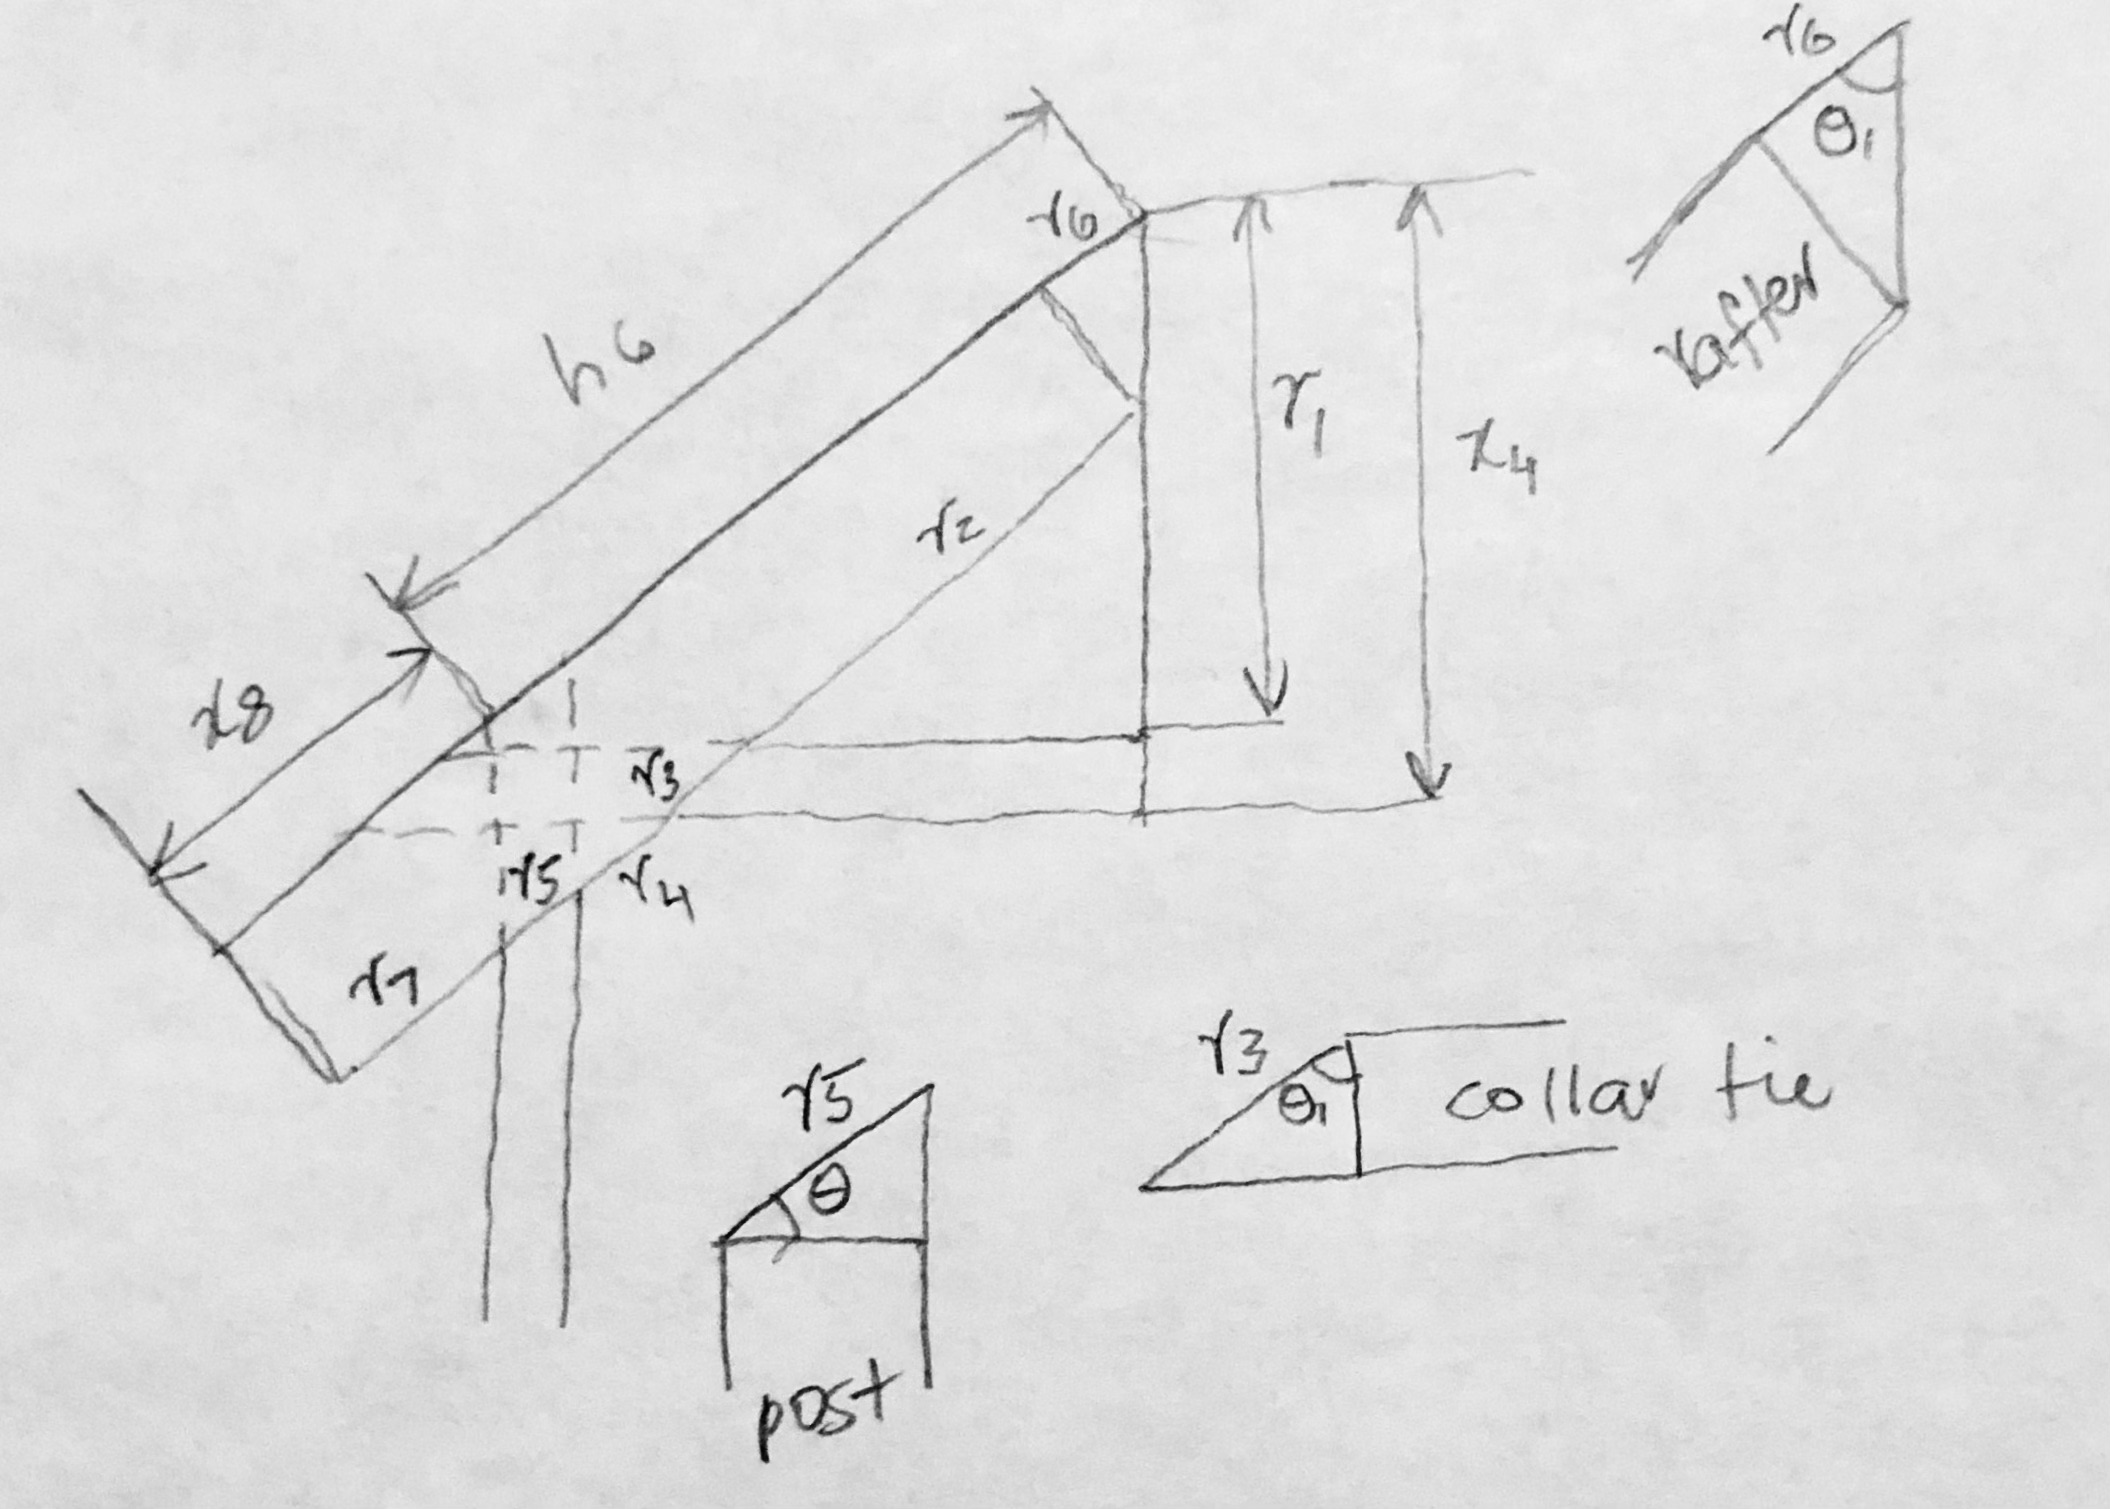
\includegraphics[width=0.5\textwidth]{images/rafter_length}
\end{center}

First, we calculate rafter length on underside, which is 
\[ r_8 = x_8 + h_6 - r_6 = x_8 + h_6 - (\text{rafter height}/\tan\theta_1) = 136.5212. \]

Then we have the following
\begin{align*}
r_3 &= \text{collar tie height}/\cos\theta_1 = 12.4964\\
r_2 &= h_3 - r_3 = 83.1838\\
r_5 &= \text{post width}/\cos\theta = 10.4137\\
r4 &= h_5 = 5.853
\end{align*}
which implies that 
\[ r_7 = r_8 - r_5 - r_4 - r_3 - r_2 = 24.5743. \]

It might seem surprising that $r_7$ = 24.5743 is more than the overhang = 24, but it does check out if drawn to scale. 

\begin{center}
	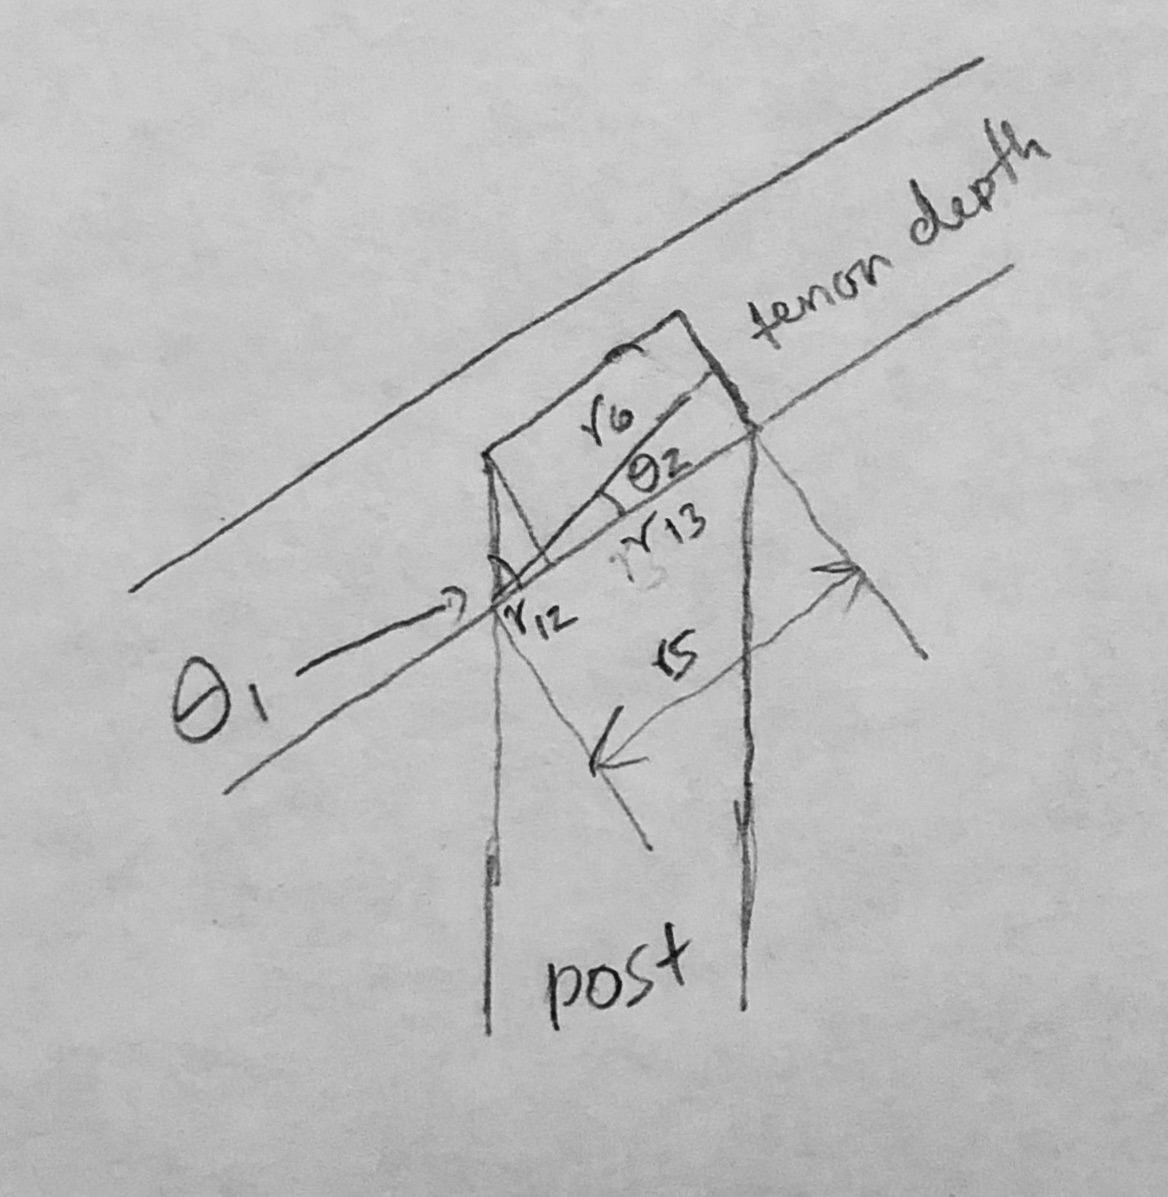
\includegraphics[width=0.5\textwidth]{images/post_tenons_into_rafters}
\end{center}

For post tenons into rafters at 2-in thick, we have 
\begin{align*}
  \theta_2 &= \arctan \left(\frac{\text{shoulder depth}}{r_5}\right) = 5.4852\\
  r_6 &= \frac{\text{shoulder depth}}{\sin\theta_2} = 10.4616\\
  r_{12} &= \frac{\text{tenon depth}}{\tan\theta_1} = 3.3333\\
  r_{13} &= r_5 - r_{12} = 7.0803
\end{align*}

\begin{center}
	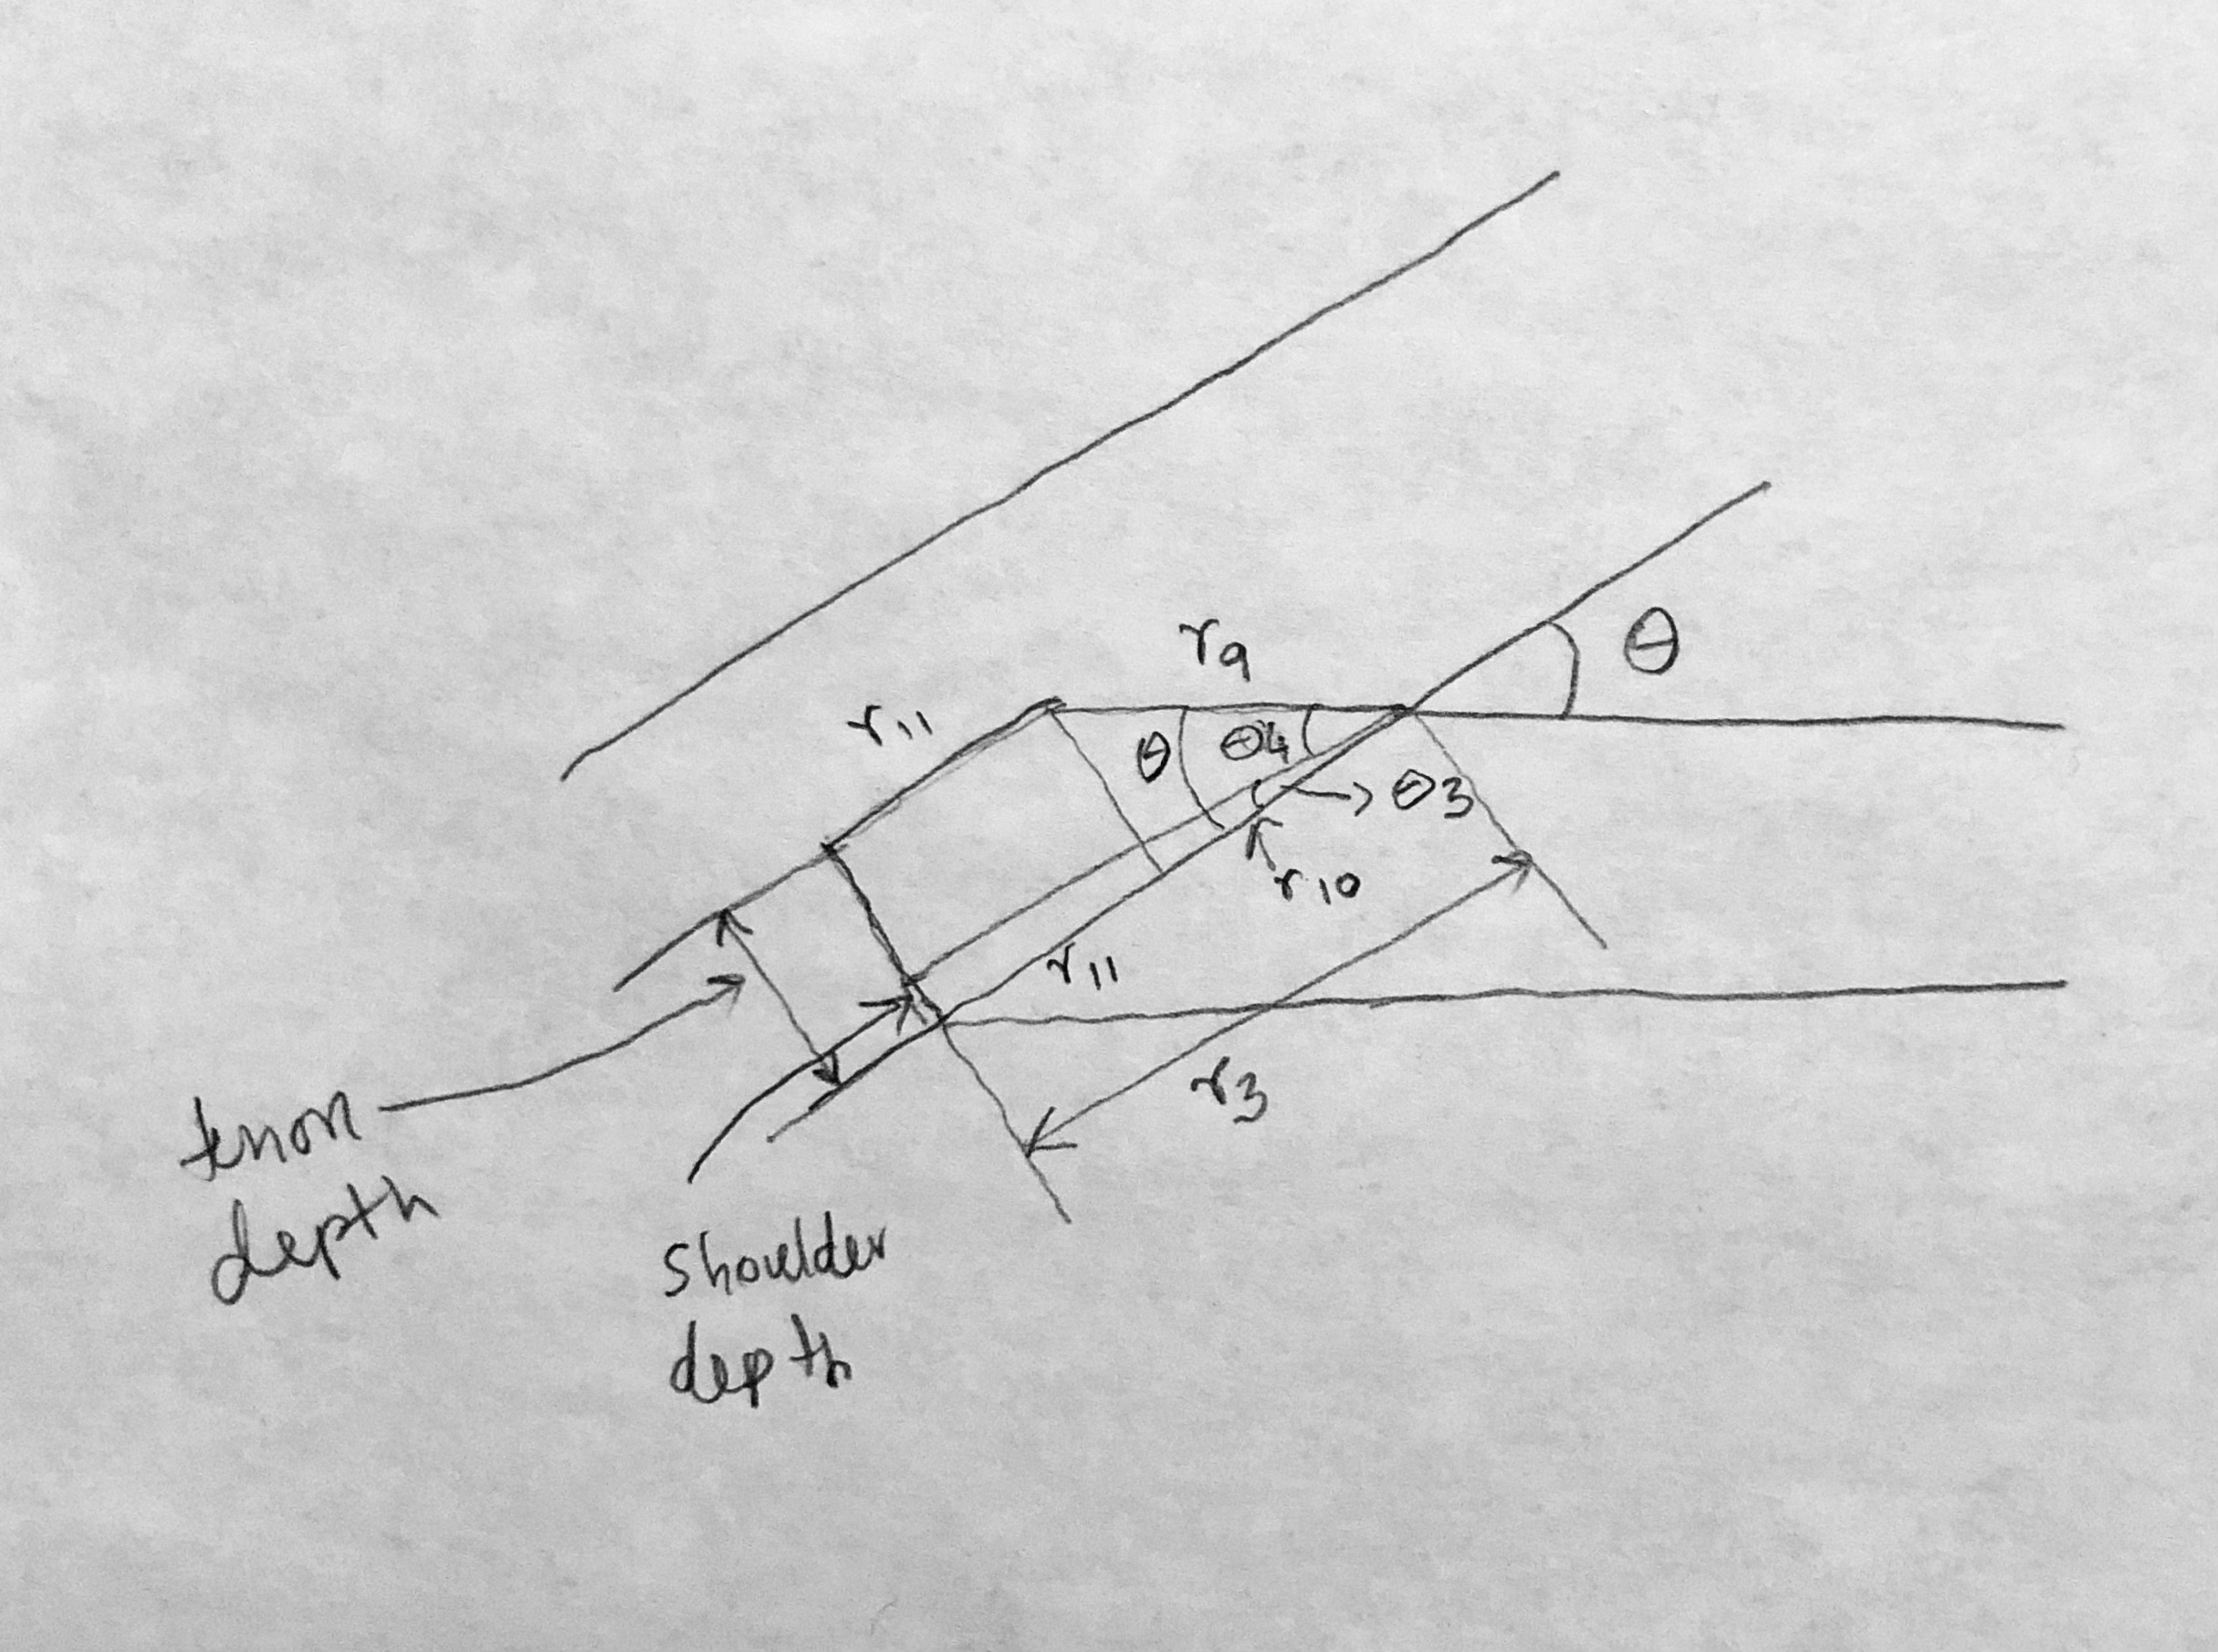
\includegraphics[width=0.5\textwidth]{images/collar_tie_tenons_into_rafters}
\end{center}

For collar tie tenons into rafters at 2-in thick, 
\begin{align*}
  \theta_3 &= \arctan \left( \frac{\text{shoulder depth}}{r_3} \right) = 4.5752^\circ\\
  \theta_4 &= \theta - \theta_3 = 35.2303^\circ\\
  r_9 &= \frac{\text{tenon depth}}{\sin\theta} = 6.2482\\
  r_{10} &= \sqrt{r_9^2 - (\text{tenon depth})^2} = 4.8\\
  r_{11} &= r_3 - r_{10} = 7.6964
\end{align*}





%%%%%%%%%%%%%%%%%%%%%%%%%%%%%%%%%%%%%%%%%%%%%%%%%%%%%%%%%%%%%%%%%%%%%%%%%%%%%%%%












\section{Strut/KP connections} \label{strut-kp-connections}

\subsection{Assumptions} \label{strut-kp-connections-assumptions}
\begin{knitrout}
\definecolor{shadecolor}{rgb}{0.969, 0.969, 0.969}\color{fgcolor}\begin{kframe}
\begin{alltt}
\hlstd{strut_height_above_collar_tie} \hlkwb{<-} \hlnum{3}
\hlstd{kp_width_bottom} \hlkwb{<-} \hlnum{10} \hlcom{# flared bottom}
\hlstd{kp_flare} \hlkwb{<-} \hlstd{(kp_width_bottom} \hlopt{-} \hlstd{kp_width)}\hlopt{/}\hlnum{2} \hlcom{# flare on each side}
\hlstd{strut_width} \hlkwb{<-} \hlnum{5}
\hlstd{strut_tenon_into_rafter_thickness} \hlkwb{<-} \hlnum{1.5}
\hlstd{strut_tenon_into_kp_depth} \hlkwb{<-} \hlnum{2}
\hlstd{strut_tenon_into_kp_thickness} \hlkwb{<-} \hlnum{1.5}
\hlstd{strut_tenon_into_rafter_depth} \hlkwb{<-} \hlnum{4}
\end{alltt}
\end{kframe}
\end{knitrout}

\subsection{Imported variables} \label{strut-kp-connections-imported-variables}
\begin{itemize}
  \item \verb+h3+ = 95.6802 from \Cref{kp-collar-tie-calculations}.
  \item \verb+collar_tie_height+ = 8 from \Cref{kp-and-collar-tie-lengths}.
  \item \verb+kp_width+ = 8 from \Cref{ridge-shape-and-dimensions-assumptions}.
  \item \verb+r2+ = 83.1838 from \Cref{rafter-lengths-connections-calculations}.
  \item \verb+r3+ = 12.4964 from \Cref{rafter-lengths-connections-calculations}.
\end{itemize}



\subsection{Calculations} \label{strut-kp-connections-calculations}


\begin{center}
	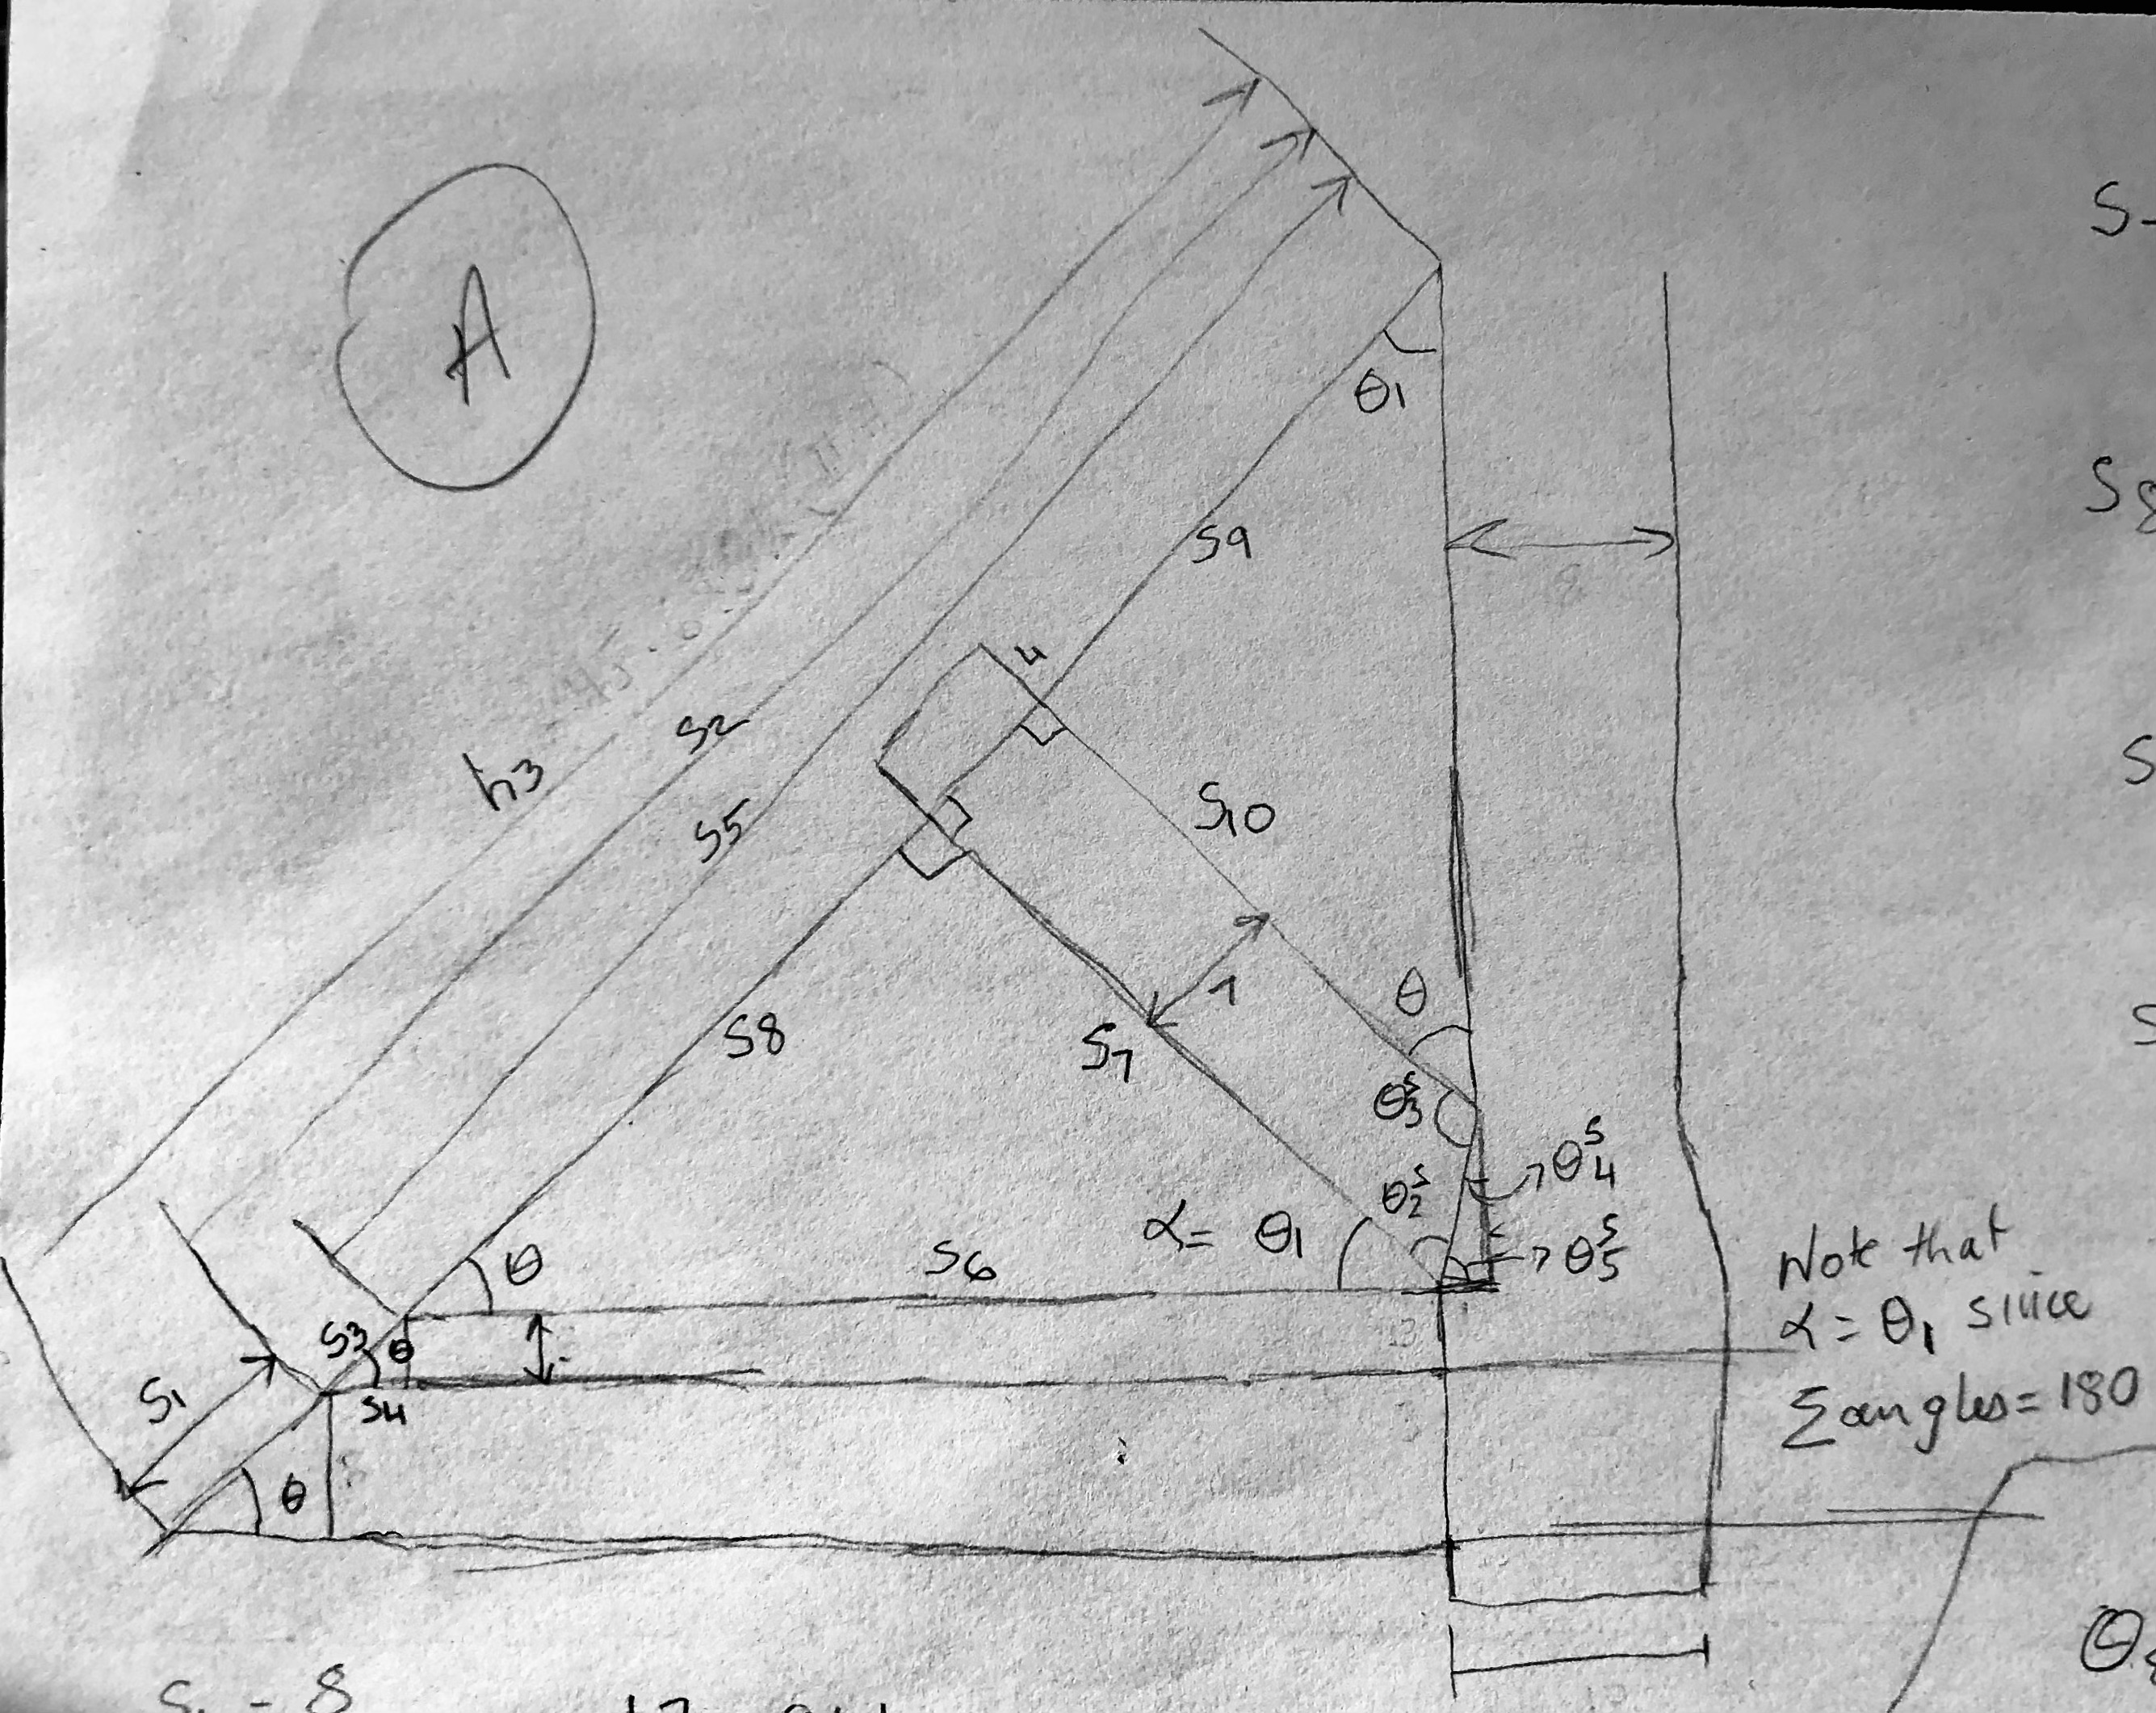
\includegraphics[width=0.5\textwidth]{images/strut_kp_overall}
\end{center}

The calculations for the first diagram are 
\begin{align*}
  s_1 &= (\text{collar tie height})/\sin\theta = 12.4964.\\
  s_2 &= h_3 - s_1 = 83.1838.\\
  s_3 &= \text{strut height above collar tie}/\sin\theta = 4.6861.\\
  s_4 &= \text{strut height above collar tie}/\tan\theta = 3.6.\\
  s_5 &= s_2 - s_3 = 78.4977.\\
  s_6 &= \cos\theta\times s_5 - \text{KP flare at bottom} = 59.3036.\\
  s_7 &= \cos\theta_1\times s_6 = 37.9652.\\
  s_8 &= \tan\theta_1\times s_7 = 45.5583.\\
  s_9 &= s_5 - s_8 - \text{strut width} = 27.9394.\\
  s_{10} &= s_9/\tan\theta = 33.5273.
\end{align*}


\begin{center}
	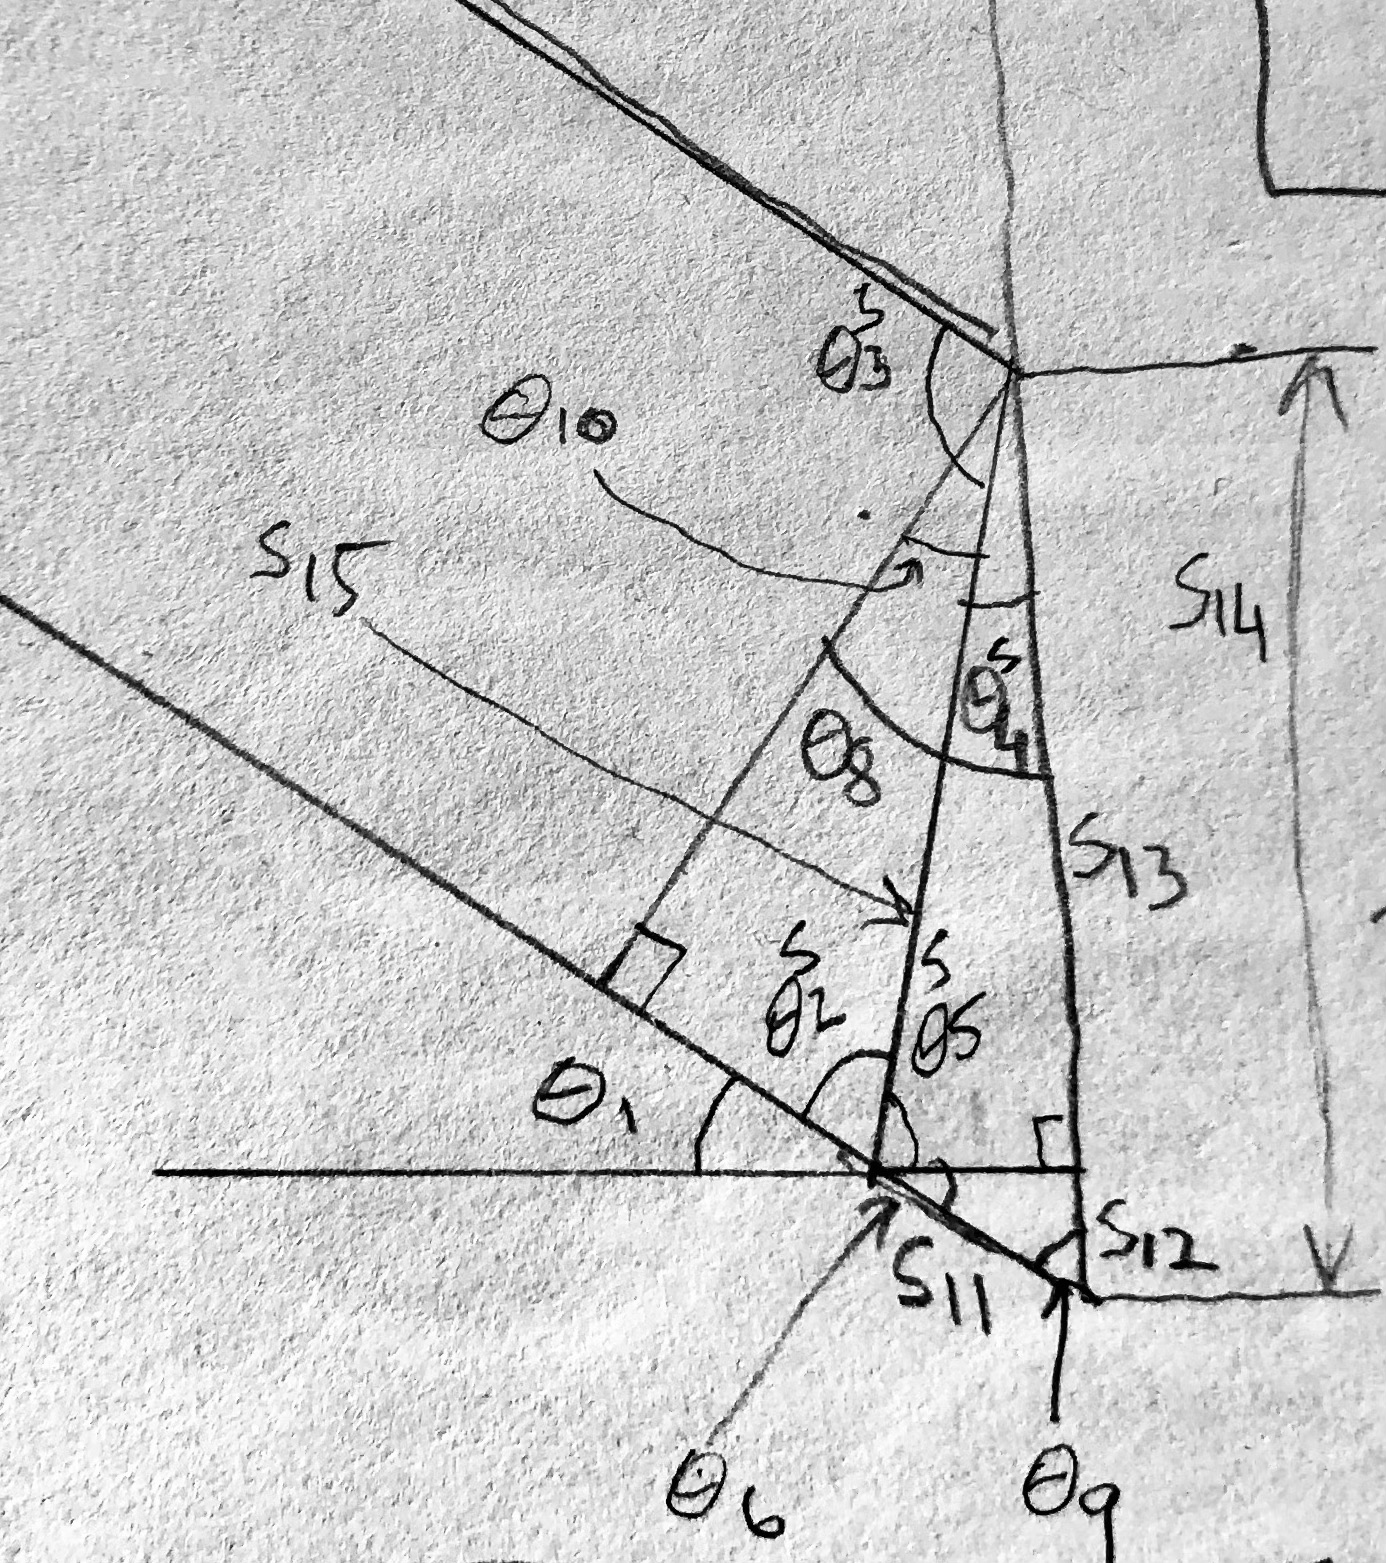
\includegraphics[width=0.35\textwidth]{images/strut_kp_detail}
\end{center}

For the second diagram, we have 
\begin{align*}
  s_{12} &= \sqrt{s_{11}^2 - \text{kp flare}^2} = 0.8333\\
  \theta_8 &= 90 - \theta_9 = \theta_1 = 50.1944\\
  s_{14} &= \text{strut width}/\cos\theta_8 = 7.8102\\
  \theta_9 &= \arcsin(\text{strut width}/s_{14}) = 39.8056\\
  s_{13} &= s_{14} - s_{12} = 6.9769\\
  s_{15} &= \sqrt{s_{13} + \text{kp flare}^2} = 7.0482\\
  \theta_5^s &= \arccos(\text{kp flare}/s_{15}) = 81.8434\\
  \theta_2^s &= \arcsin(\text{strut width}/s_{15}) = 45.1861\\
  \theta_4^s &= \arcsin(\text{kp flare}/s_{15}) = 8.1566\\
  \theta_{10} &= \arccos(\text{strut width}/s_{15}) = 44.8139\\
  \theta_3^s &= 90 + \theta_{10} = 134.8139
\end{align*}

\begin{center}
\fbox{\textbf{Check: Does $s_2 = r_2$?} TRUE.}
\end{center}

\begin{center}
\fbox{\textbf{Check: Does $s_1 = r_3$?} TRUE.}
\end{center}

\begin{center}
\fbox{\textbf{Check: Does $\theta_9 = \theta$?} TRUE.}
\end{center}



\subsection{Strut tenons into KP}
\begin{center}\fbox{There seems to be an extra $s_{18}$ in the diagram in the middle - not sure what that is.}\end{center}
\begin{center}
	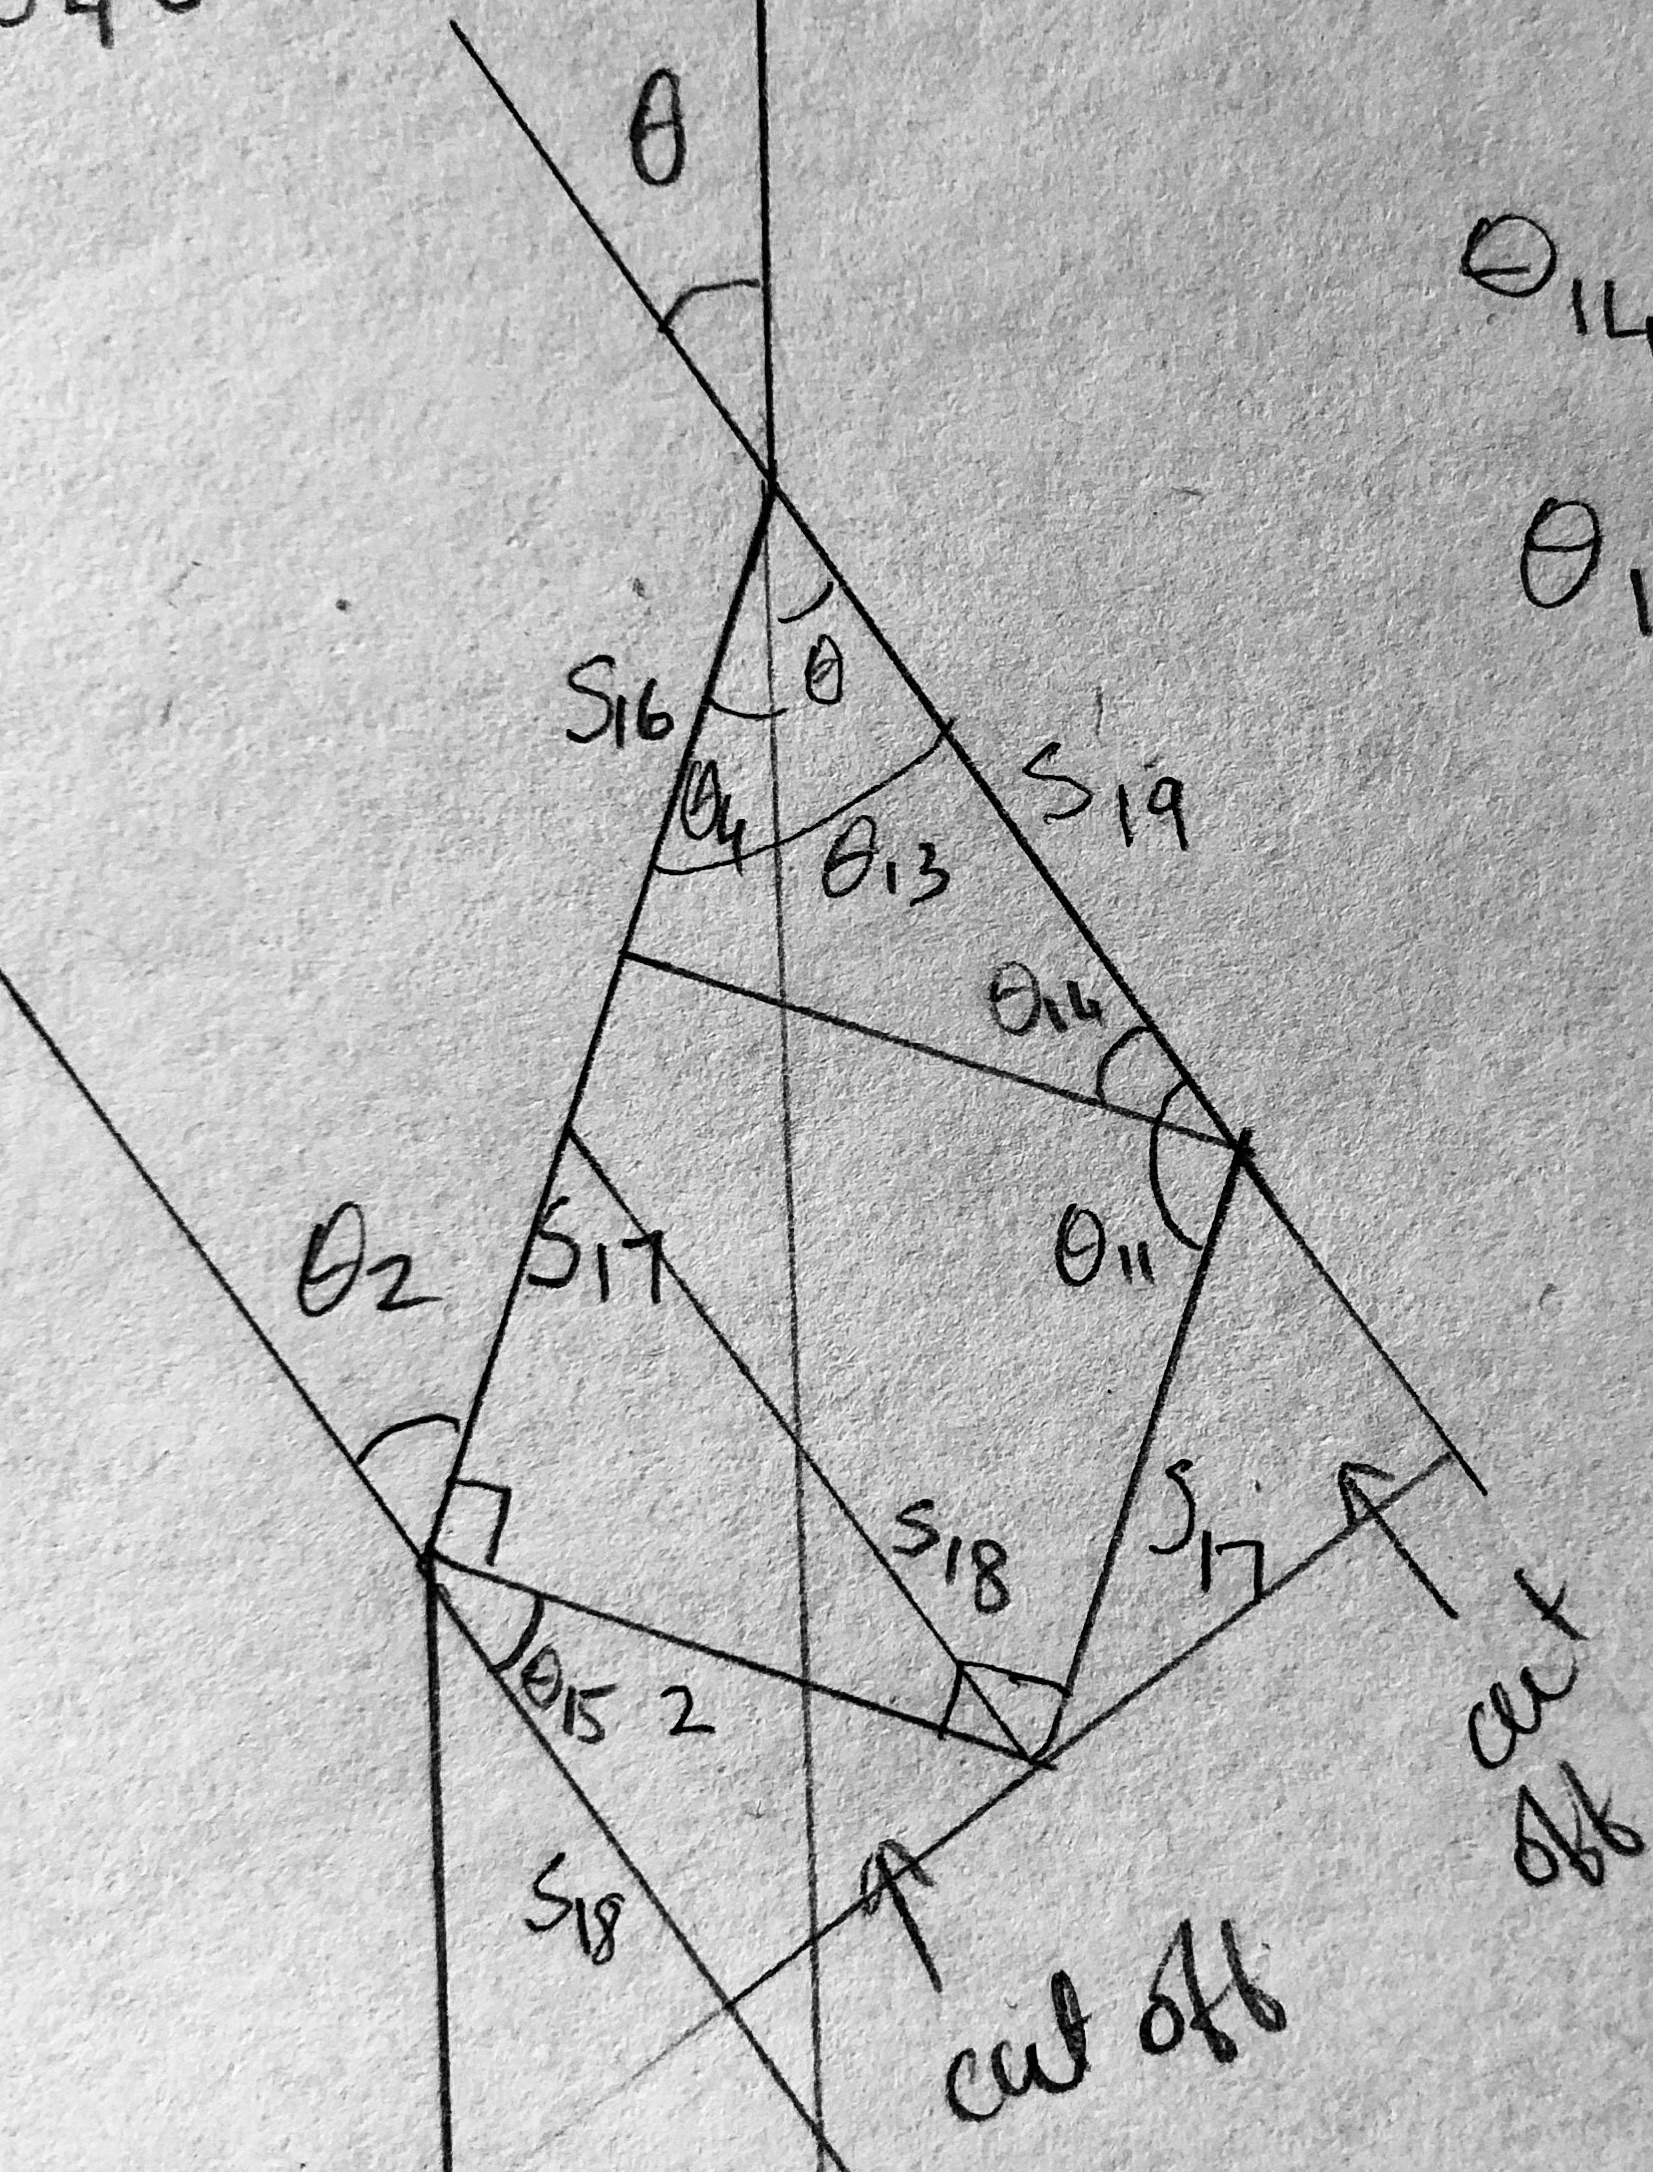
\includegraphics[width=0.45\textwidth]{images/strut_kp_tenon_detail}
\end{center}

The calculations are 
\begin{align*}
  \theta_{13} &= \theta + \theta_4^2 = 47.9622\\
  \theta_{11} &= 360 - 90 - 90 - \theta_{13} = 132.0378\\
  s_{19} &= \text{strut tenon into kp depth}/\sin\theta_{13} = 2.6929\\
  \theta_{14} &= \theta_{11} - 90 = 42.0378\\
  \theta_{15} &= 180 - \theta_s^2 - 90 = 44.8139\\
  s_{16} &= \sqrt{s_{19}^2 - \text{strut tenon into kp depth}^2} = 1.8032\\
  s_{17} &= s_{15} - s_{16} = 5.245\\
  s_{18} &= \cos\theta_{15}\times \text{strut tenon into kp depth} = 1.4188
\end{align*}












%%%%%%%%%%%%%%%%%%%%%%%%%%%%%%%%%%%%%%%%%%%%%%%%%%%%%%%%%%%%%%%%%%%%%%%%%%%%%%%%







\section{Collar tie final length}\label{collar-tie-final-length}

\subsection{Assumptions}
\begin{knitrout}
\definecolor{shadecolor}{rgb}{0.969, 0.969, 0.969}\color{fgcolor}\begin{kframe}
\begin{alltt}
\hlstd{collar_tie_tenon_into_rafter_depth} \hlkwb{<-} \hlnum{4} \hlcom{# at 90 degrees to rafter face}
\hlstd{collar_tie_depth} \hlkwb{<-} \hlnum{6} \hlcom{# beam depth}
\hlstd{kp_through_tenon_thickness} \hlkwb{<-} \hlnum{2}
\end{alltt}
\end{kframe}
\end{knitrout}

\subsection{Imported variables}
\begin{itemize}
  \item \verb+x2+ = 73.5036 from \Cref{kp-collar-tie-calculations}
  \item \verb+kp_flare+ = 1 from \Cref{strut-kp-connections-assumptions}
  \item \verb+kp_width_bottom+ = 10 from \Cref{strut-kp-connections-assumptions}
  \item \verb+r11+ = 7.6964 from \Cref{rafter-lengths-connections-calculations}
  \item \verb+r9+ = 6.2482 from \Cref{rafter-lengths-connections-calculations}
  \item \verb+collar_tie_height+ = 8 from \Cref{kp-collar-tie-assumptions}
  \item \verb+collar_tie_rafter_shoulder_depth+ = 1 from \Cref{rafter-lengths-connections-assumptions}
  \item \verb+collar_tie_tenon_into_rafter_thickness+ = 2 from \Cref{rafter-lengths-connections-assumptions}
  \item \verb+kp_width+ = 8 from \Cref{ridge-shape-and-dimensions-assumptions}
  \item \verb+theta3_degrees+ = 4.5752 from \Cref{rafter-lengths-connections-calculations}
\end{itemize}

\subsection{Calculations}



\begin{center}\fbox{\textbf{TODO - SEE PAPER FOR THE d AND cc variables - feb 21 2024}}\end{center}


14.4018


\begin{center}\fbox{The diagram has a hardcoded value - ignore.}\end{center}
\begin{center}
	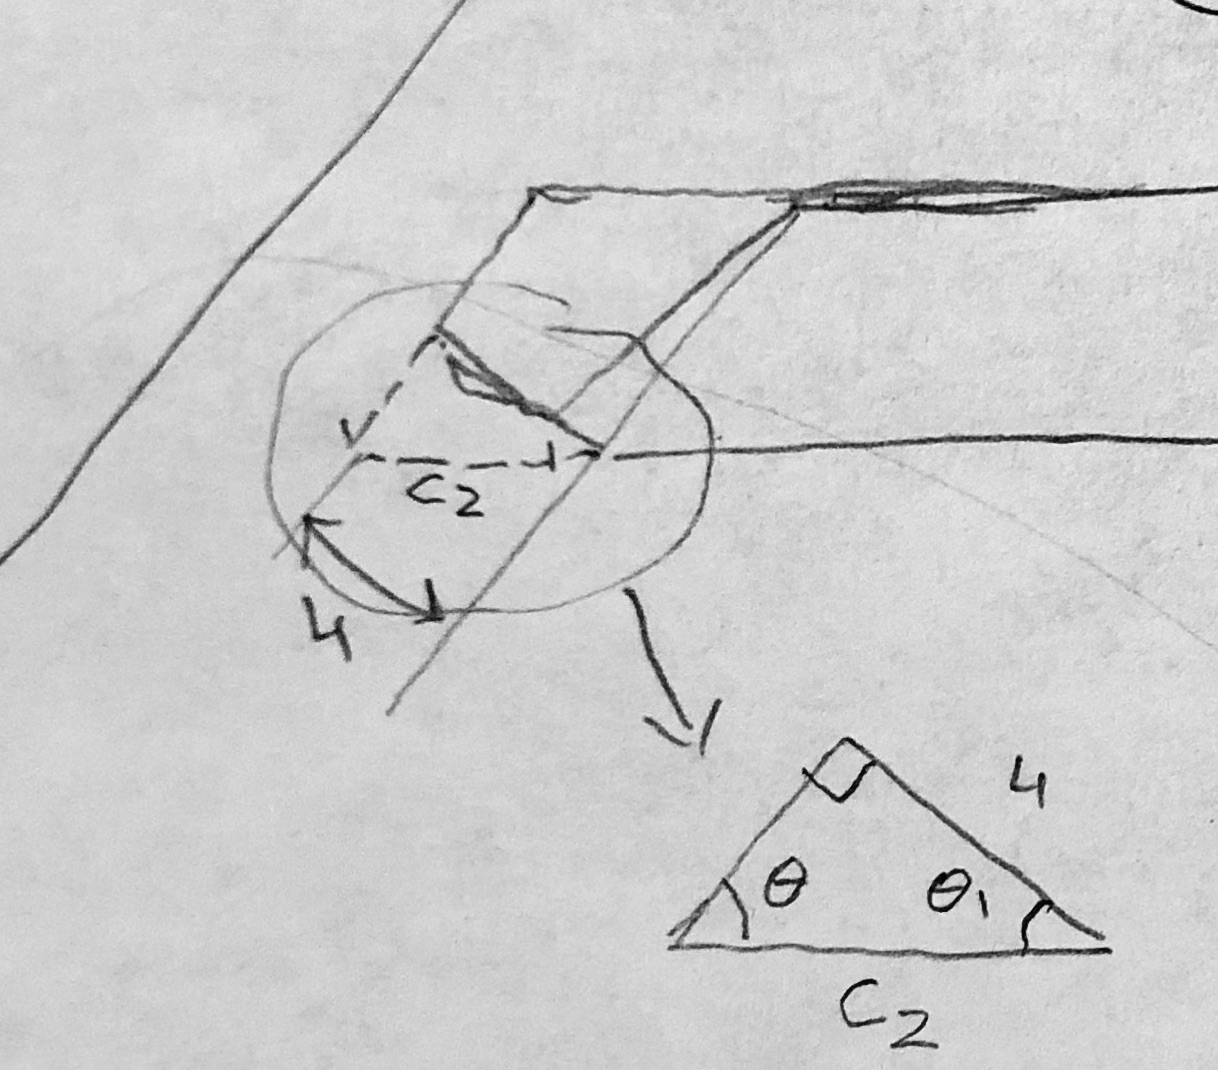
\includegraphics[width=0.45\textwidth]{images/ct_cut_plan}
\end{center}

Since tenon depth = 4, we have $c_2$ = 6.2482. Since KP width at bottom is 10, we modify from above (\Cref{ridge-shape-and-dimensions-assumptions}) where KP width was 8 (\Cref{ridge-shape-and-dimensions-assumptions}):
\[ \text{New }x_2 = c_1 = x_2 - 1 = 72.5036.  \]

Then 
\[ \boxed{\text{CT length }= c_1\times 2 + 10 + c_2\times 2 = 167.5036 = \text{13' 11" 1/2}.}\]








%%%%%%%%%%%%%%%%%%%%%%%%%%%%%%%%%%%%%%%%%%%%%%%%%%%%%%%%%%%%%%%%%%%%%%%%%%%%%%%%









\section{Braces} \label{braces}

\subsection{Assumptions}
\begin{knitrout}
\definecolor{shadecolor}{rgb}{0.969, 0.969, 0.969}\color{fgcolor}\begin{kframe}
\begin{alltt}
\hlstd{brace_width} \hlkwb{<-} \hlnum{5}
\hlstd{brace_exposed_length_top} \hlkwb{<-} \hlnum{36}
\hlstd{brace_tenon_depth_into_collar_tie} \hlkwb{<-} \hlnum{3}
\hlstd{brace_tenon_depth_into_post} \hlkwb{<-} \hlnum{3}
\end{alltt}
\end{kframe}
\end{knitrout}
\subsection{Imported variables}
\begin{itemize}
  \item \verb+x5+ = 4.4964 from \Cref{kp-collar-tie-calculations}.
  \item \verb+r4+ = 5.853 from \Cref{rafter-lengths-connections-calculations}.
\end{itemize}

\subsection{Calculations} \label{braces-calculations}


\begin{center}\fbox{The diagrams have some hardcoded values - ignore those.}\end{center}

\begin{center}
	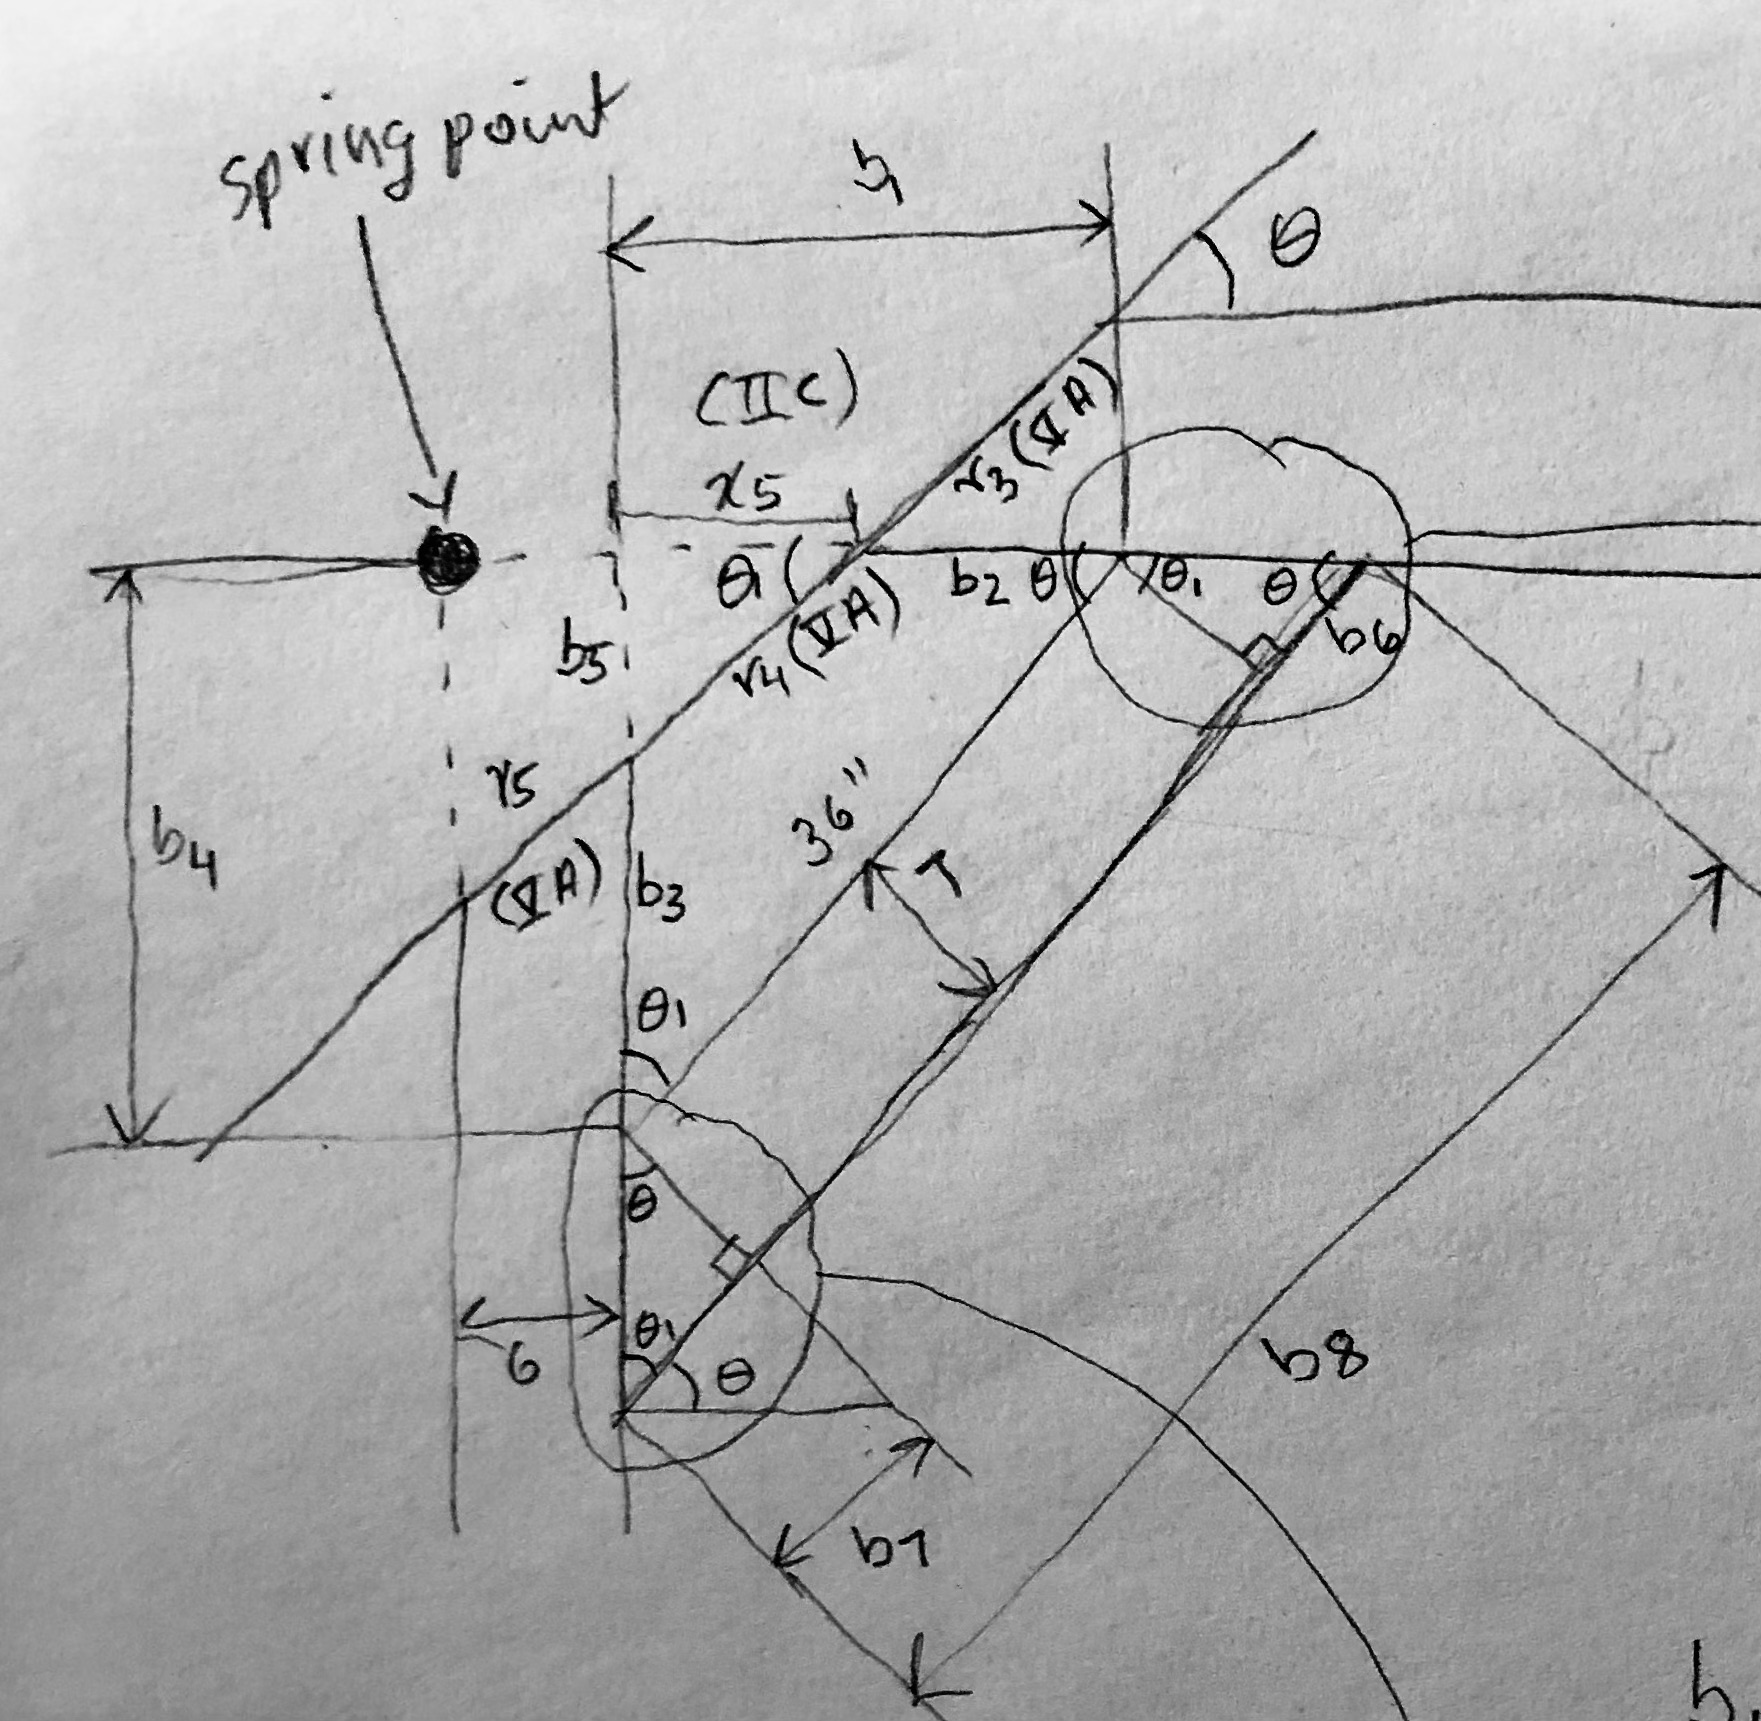
\includegraphics[width=0.45\textwidth]{images/braces_overall}
\end{center}

For the overall diagram, the calculations are
\begin{align*}
  b_1 &= \cos\theta\times \text{brace exposed length at top} = 27.656\\
  b_2 &= b_1 - x_5 = 23.1596\\
  b_5 &= \sin\theta_1\times r_4 = 4.4964\\
  b_4 &= \sin\theta\times \text{brace exposed length at top} = 23.0466\\
  b_3 &= b_4 - b_5 = 18.5502\\
  b_6 &= \tan\theta_1\times \text{brace width} = 6\\
  b_7 &= \tan\theta\times \text{brace width} = 4.1667\\
  b_8 &= \text{brace exposed length at top} + b_6 + b_7 = 46.1667\\
\end{align*}

\begin{center}
	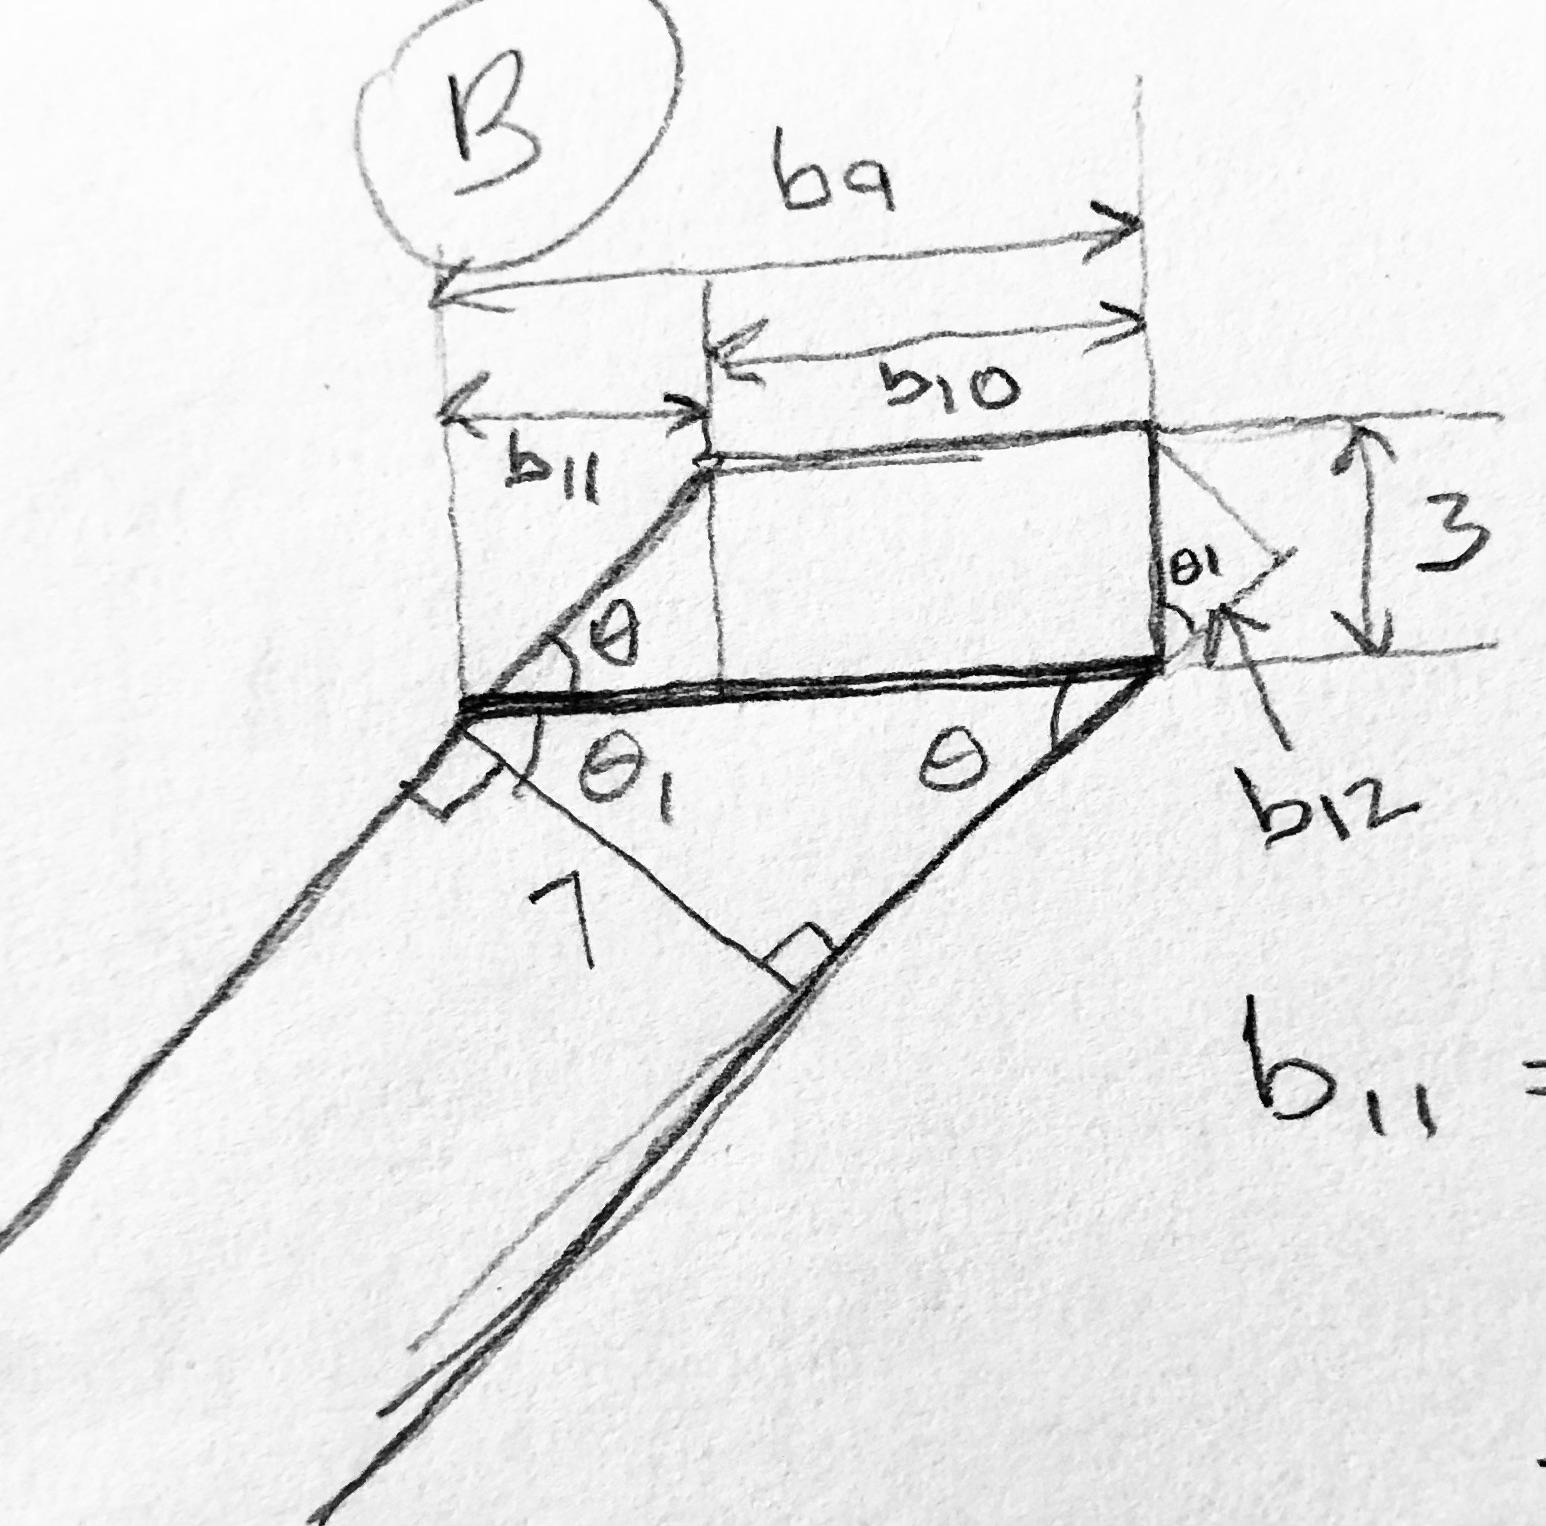
\includegraphics[width=0.45\textwidth]{images/braces_into_ct}
\end{center}

For braces into collar tie, 
\begin{align*}
  b_{11} &= \text{brace tenon depth into collar tie}/\tan\theta = 3.6\\
  b_9 &= \text{brace width}/\cos\theta_1 = 7.8102\\
  b_{10} &= b_9 - b_{11} = 4.2102\\
  b_{12} &= \text{brace tenon depth into collar tie}\times \cos\theta_1 = 1.9206\\
\end{align*}

\begin{center}
	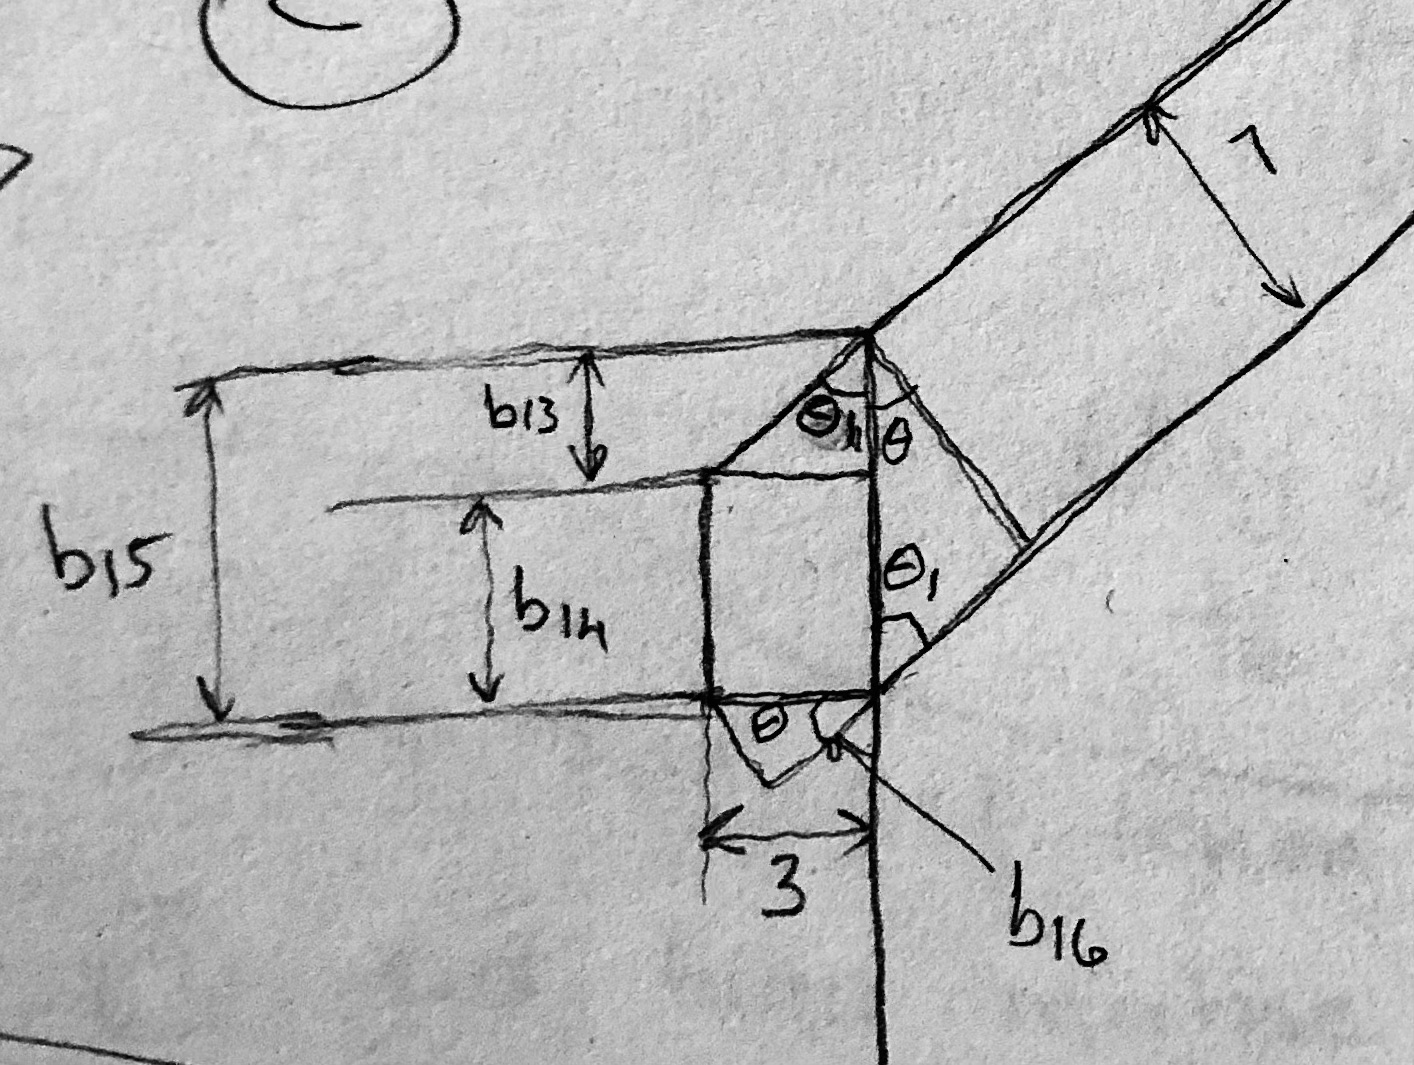
\includegraphics[width=0.45\textwidth]{images/braces_into_post}
\end{center}

For braces into post, 
\begin{align*}
  b_{13} &= \text{brace tenon depth into post}/\tan\theta_1 = 2.5\\
  b_{15} &= \text{brace width}/\cos\theta = 6.5085\\
  b_{14} &= b_{15} - b_{13} = 4.0085\\
  b_{16} &= \cos\theta\times \text{brace tenon depth into post} = 2.3047
\end{align*}







%%%%%%%%%%%%%%%%%%%%%%%%%%%%%%%%%%%%%%%%%%%%%%%%%%%%%%%%%%%%%%%%%%%%%%%%%%%%%%%%










\section{Posts}\label{posts-plan}
\begin{wrapfigure}[25]{r}{0.5\textwidth}
  \begin{center}
  	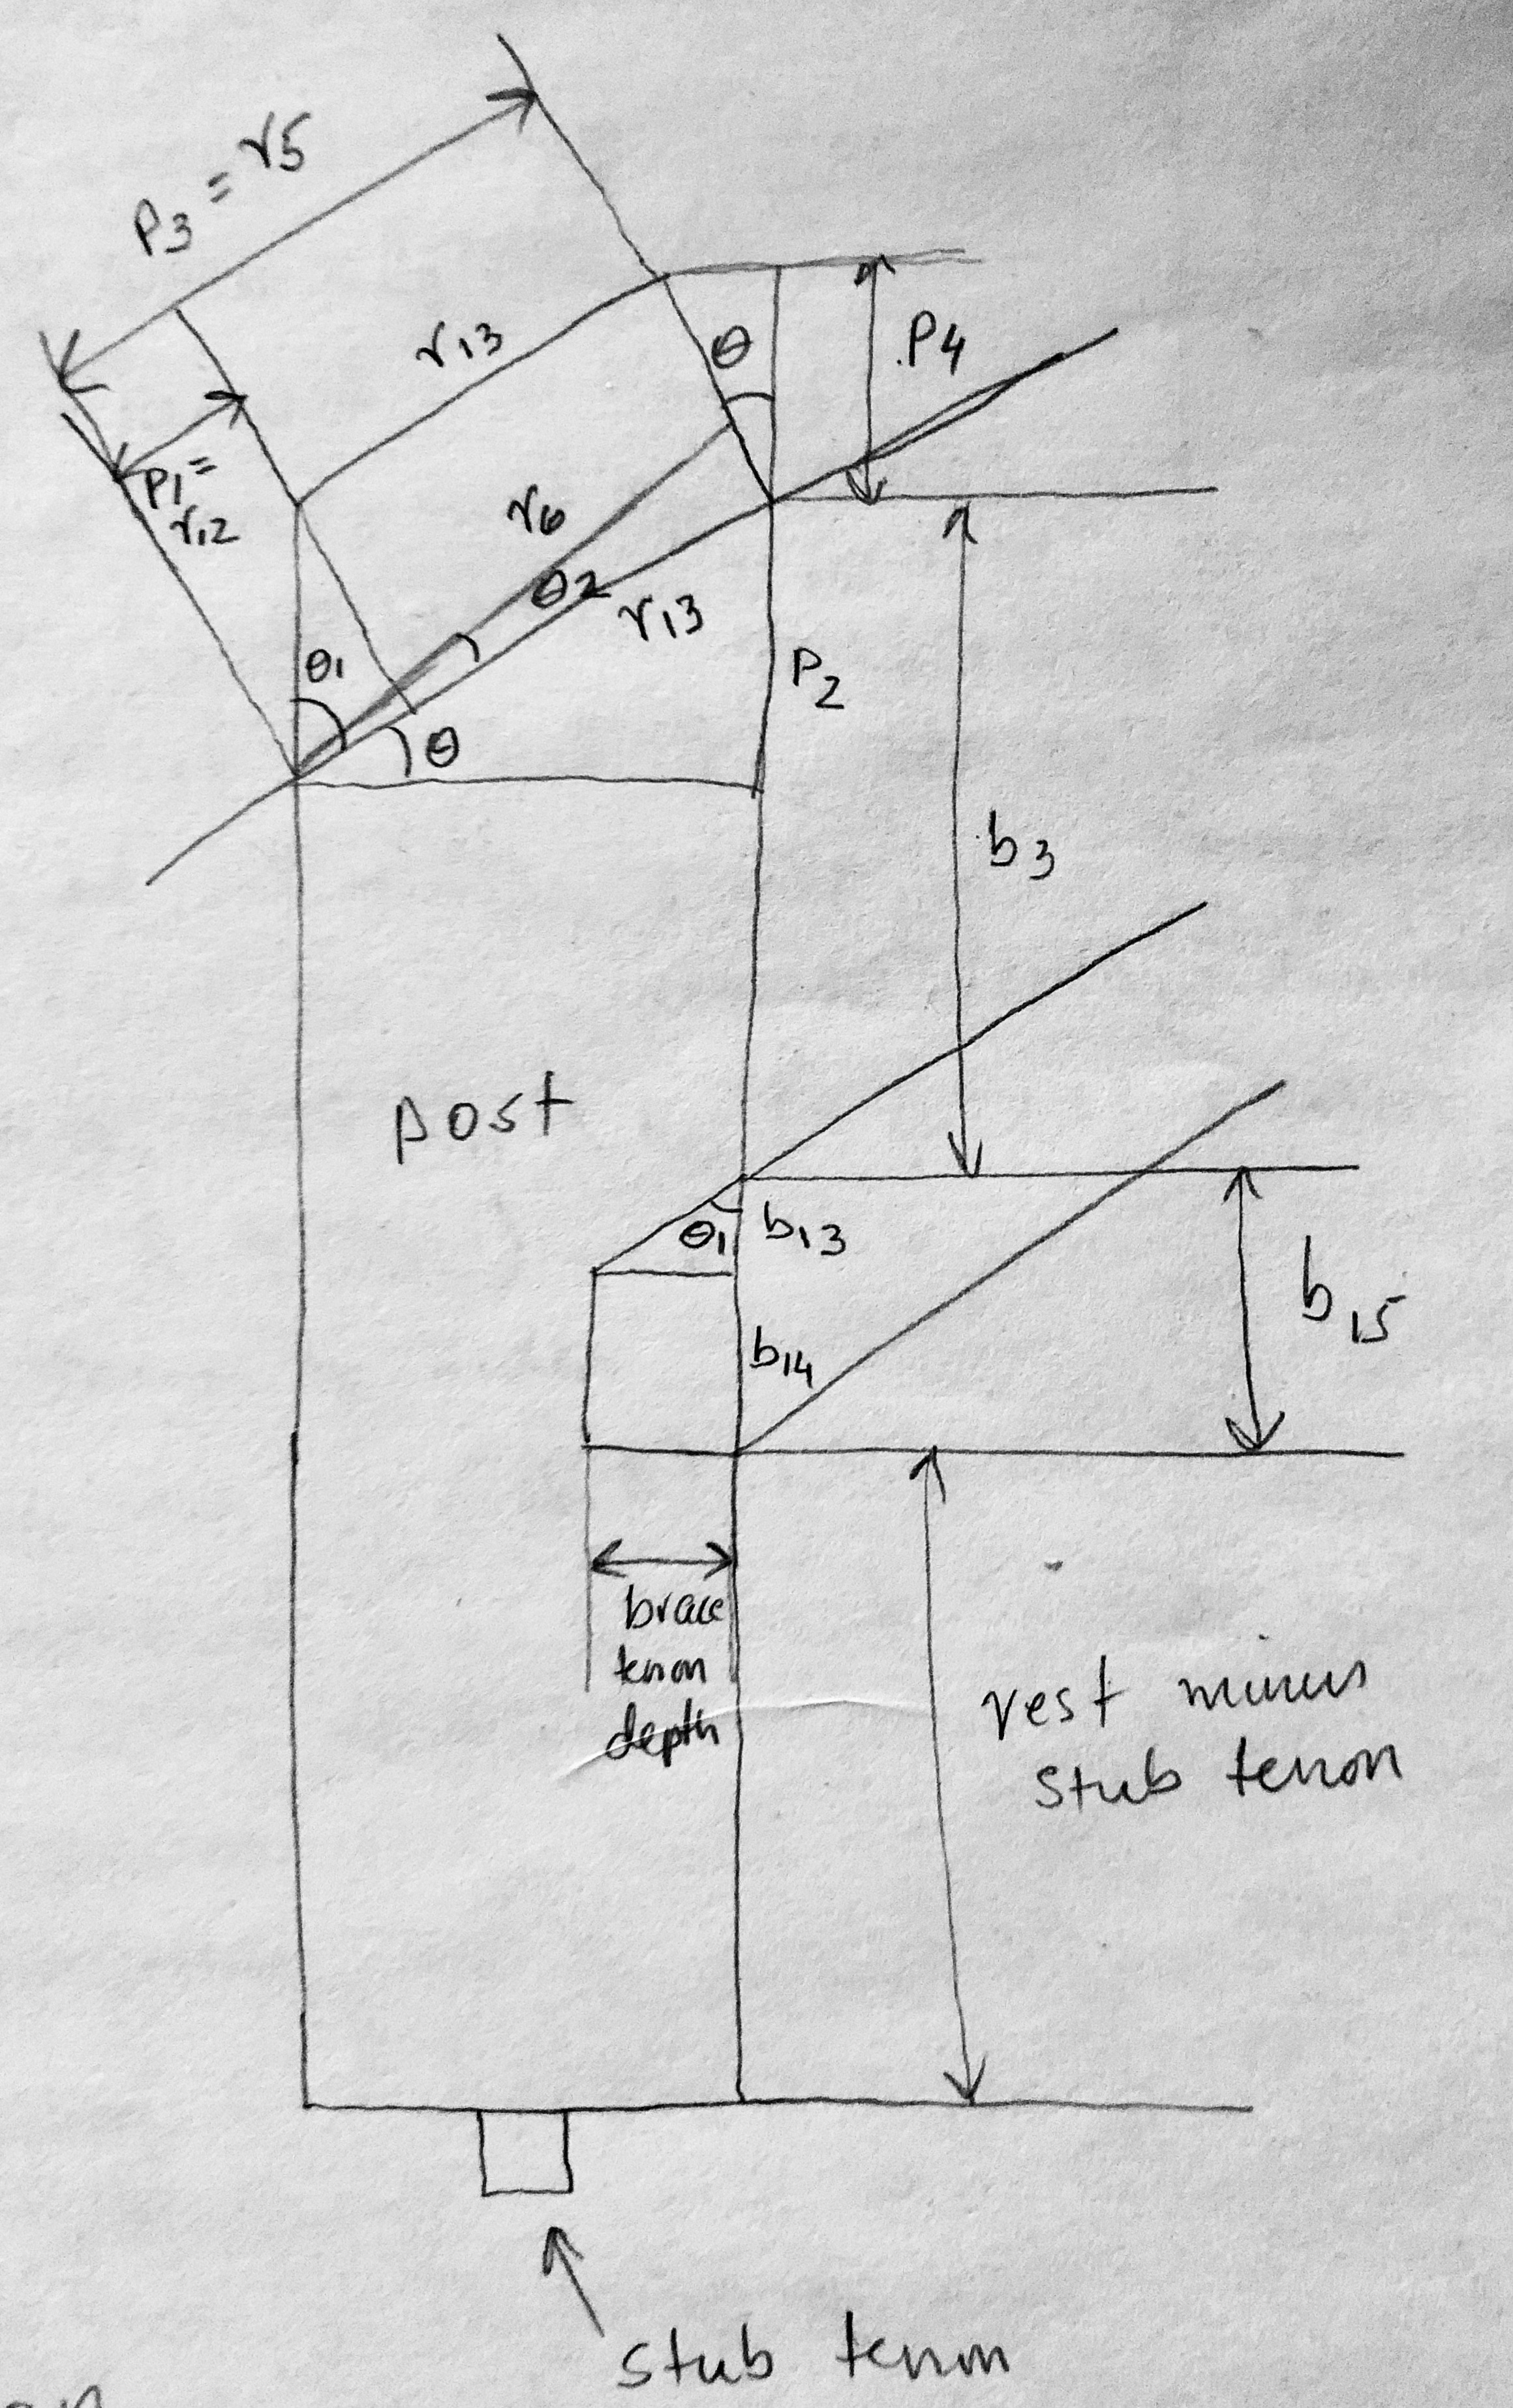
\includegraphics[width=0.5\textwidth]{images/post_calculations}
  \end{center}
	\caption{Posts layout}
\end{wrapfigure}

\subsection{Assumptions} \label{posts-plan-assumptions}
\begin{knitrout}
\definecolor{shadecolor}{rgb}{0.969, 0.969, 0.969}\color{fgcolor}\begin{kframe}
\begin{alltt}
\hlstd{post_stub_tenon_length} \hlkwb{<-} \hlnum{2}
\end{alltt}
\end{kframe}
\end{knitrout}
\subsection{Imported variables}
Imports: 
% This word is here just so wrapfig works correctly
\begin{itemize}
  \item \verb+post_tenon_depth_into_rafter+ = 4 from \Cref{rafter-lengths-connections-assumptions}. 
  \item \verb+r12+ = 3.3333 from \Cref{rafter-lengths-connections-calculations}, here called $p_1$. 
  \item \verb+r5+ = 10.4137 from \Cref{rafter-lengths-connections-calculations}, here called $p_3$. 
  \item \verb+post_width+ = 8 from \Cref{kp-collar-tie-assumptions}. 
  \item \verb+post_tenon_depth_into_rafter+ = 4 from \Cref{rafter-lengths-connections-assumptions}.
  \item \verb+post_height_excluding_tenons+ = 93.4428 from \Cref{posts-rafters-calculations}.
  \item \verb+b3+ = 18.5502 from \Cref{braces-calculations}. 
  \item \verb+b15+ = 6.5085 from \Cref{braces-calculations}. 
\end{itemize}

\subsection{Calculations} \label{posts-plan-calculations}



Some of the calculations were covered above in \Cref{rafter-lengths-and-connections} from the perspective of the mortise. Here, we concentrate on the tenons. Some variables are imports from the section mentioned. For the others, 
\begin{align*}
  p_2 &= \sqrt{p_3^2 - \text{post width}^2} = 6.6667\\
  p_4 &= \cos\theta\times\text{post tenon depth into rafter} = 3.0729
\end{align*}

From \Cref{posts-rafters-calculations}, post height excluding tenons is 93.4428, so total post height = post height excluding tenons + stub tenon length + $p_4$, which is 

\[ \boxed{98.5156 = \text{8' 2" 17/32}.} \]











%%%%%%%%%%%%%%%%%%%%%%%%%%%%%%%%%%%%%%%%%%%%%%%%%%%%%%%%%%%%%%%%%%%%%%%%%%%%%%%%






\newpage

\section{Cut plans}

\begin{center}
  \fbox{Calibrate all measuring instruments against each other before starting.}
\end{center}
\newpage

\subsection{Posts}

% \subsubsection{Assumptions} \label{posts-cut-plan-assumptions}


% \subsubsection{Imported variables}
% \begin{itemize}
%   \item \verb+post_width+ = post_width from \Cref{kp-collar-tie-assumptions}. 
%   \item \verb+post_height_total_imperial+ = post_height_total_imperial from \Cref{posts-plan-calculations}.
%   \item \verb+p4+ = p4 from \Cref{posts-plan-calculations}.
%   \item \verb+b3+ = b3 from \Cref{braces-calculations}. 
%   \item \verb+b15+ = b15 from \Cref{braces-calculations}. 
%   \item \verb+post_rest_minus_stub+ = post_rest_minus_stub from \Cref{posts-plan-calculations}.
%   \item \verb+b13+ = b13 from \Cref{braces-calculations}.
%   \item \verb+b14+ = b14 from \Cref{braces-calculations}.
% \end{itemize}

\begin{wrapfigure}[20]{r}{0.5\textwidth}
  \begin{center}
  	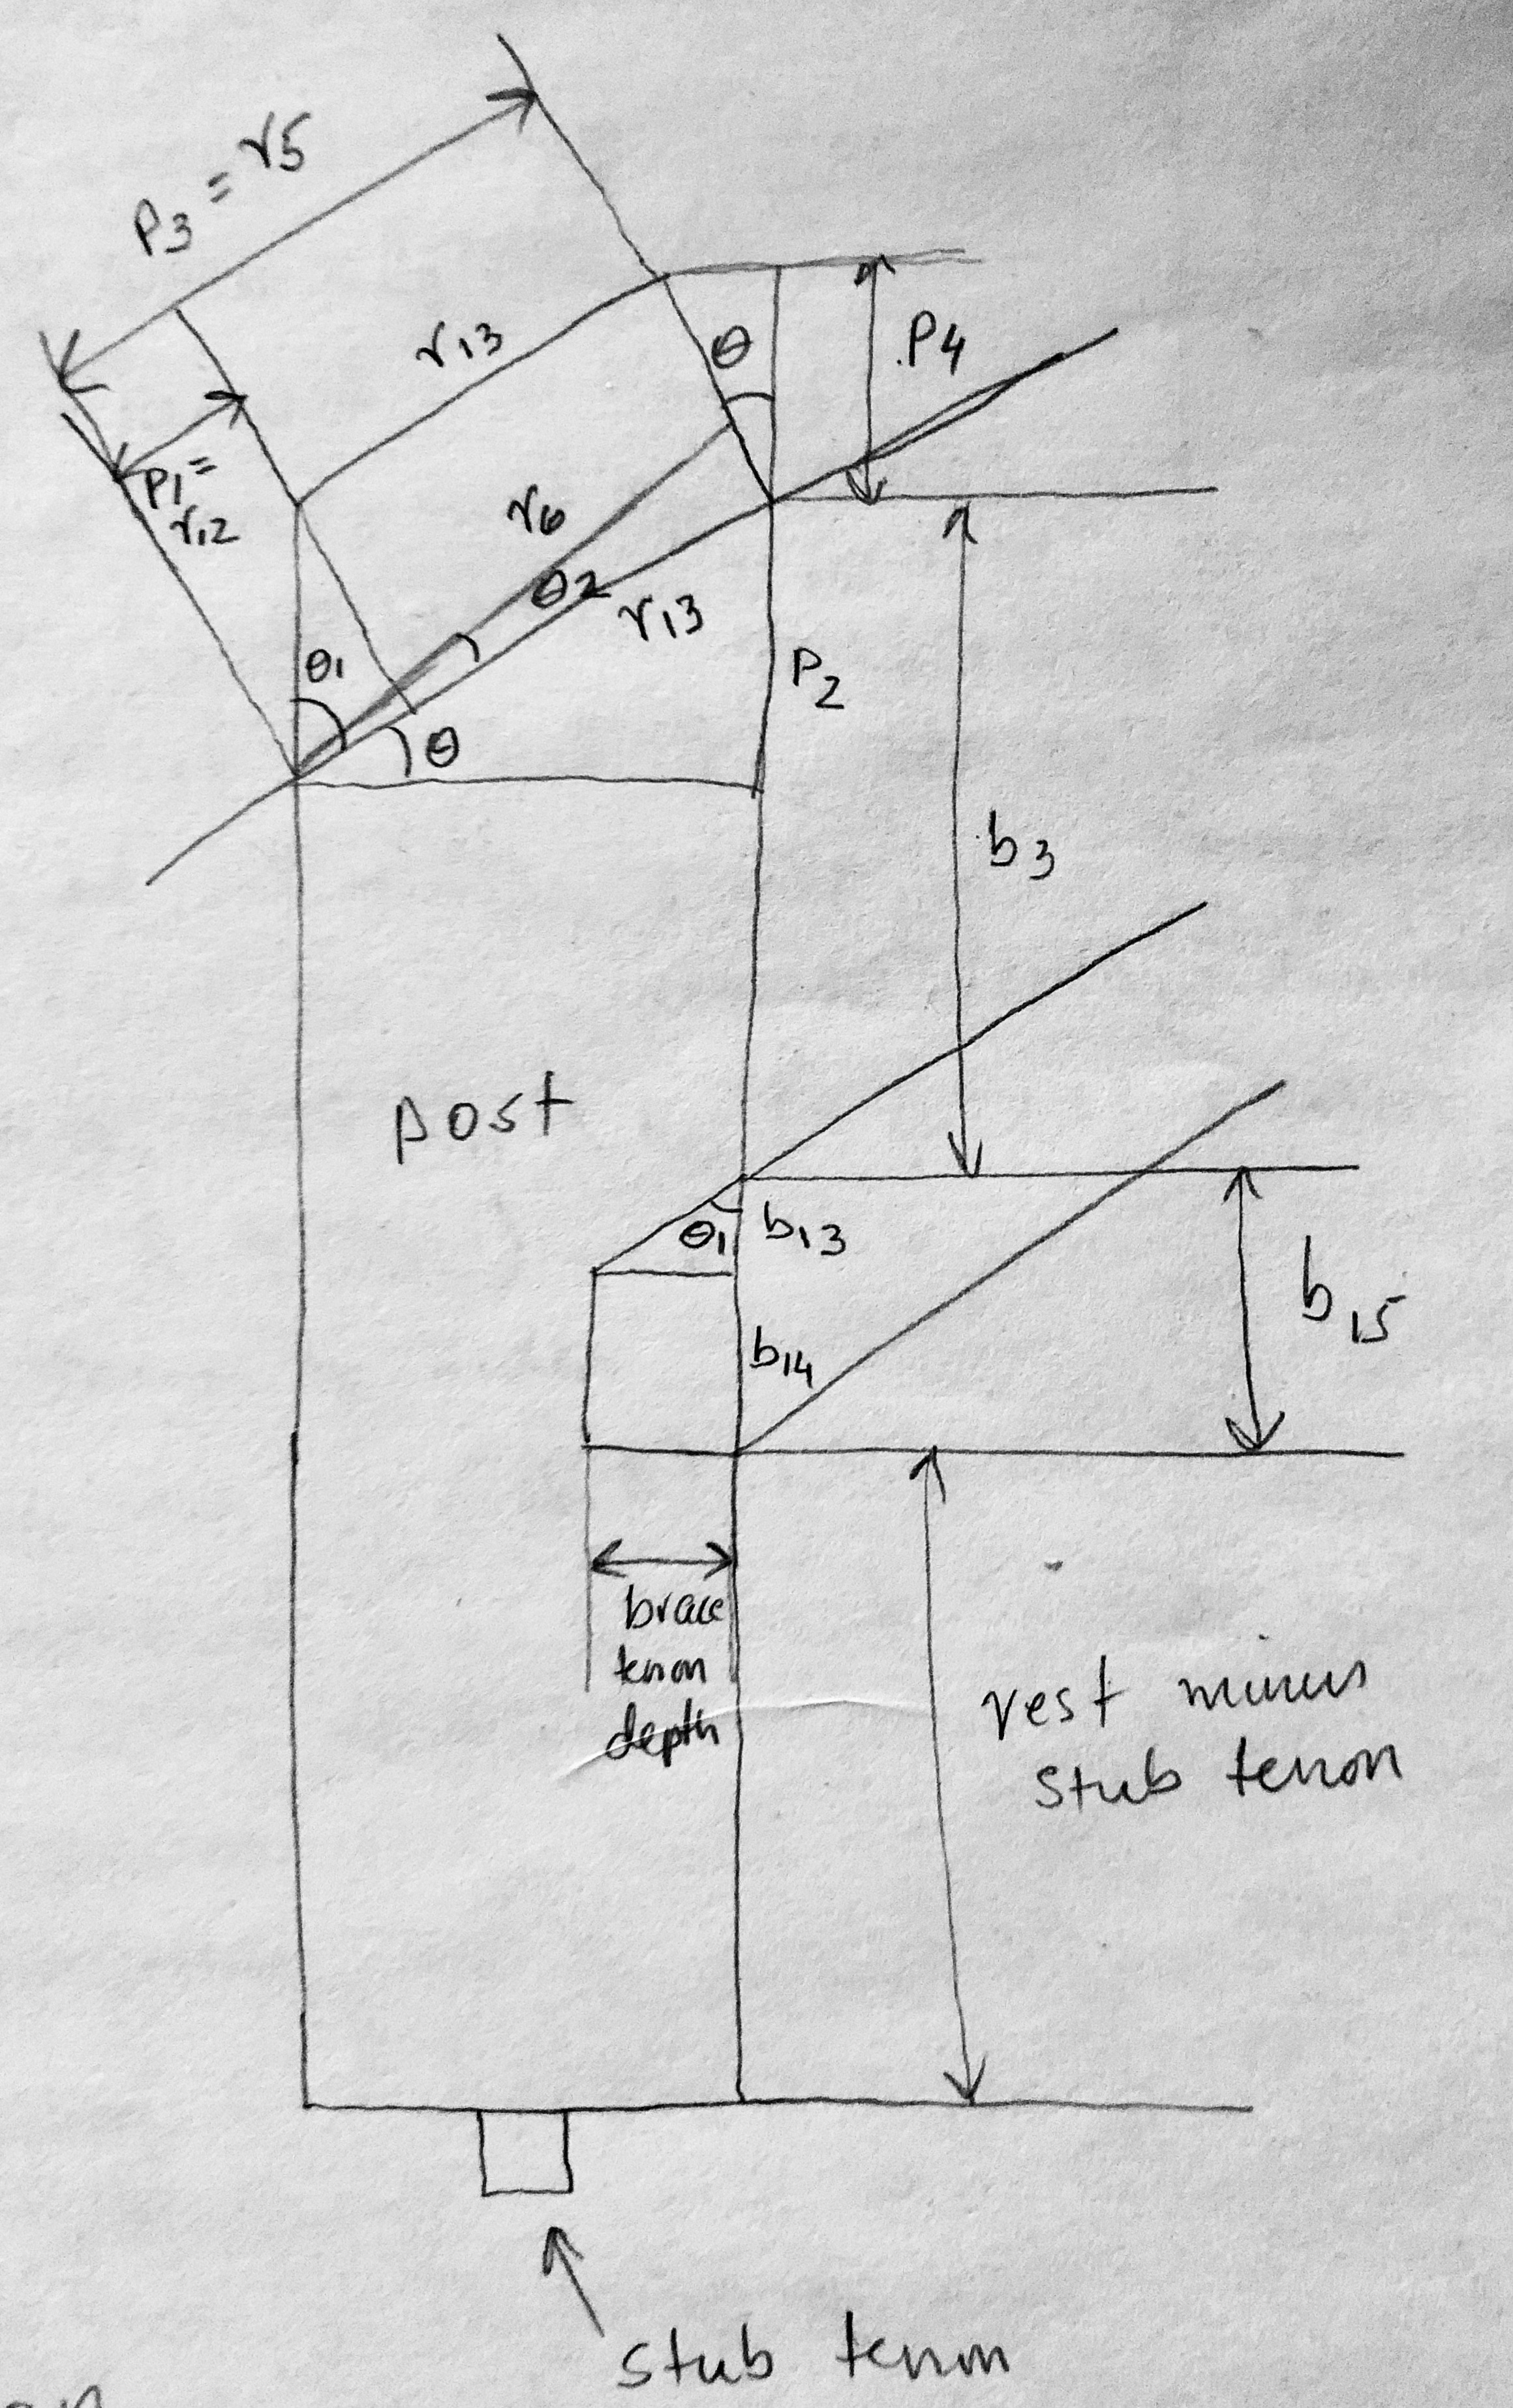
\includegraphics[width=0.5\textwidth]{images/post_calculations}
  \end{center}
	\caption{Posts layout}
\end{wrapfigure}

% 
% \begin{center}
% 	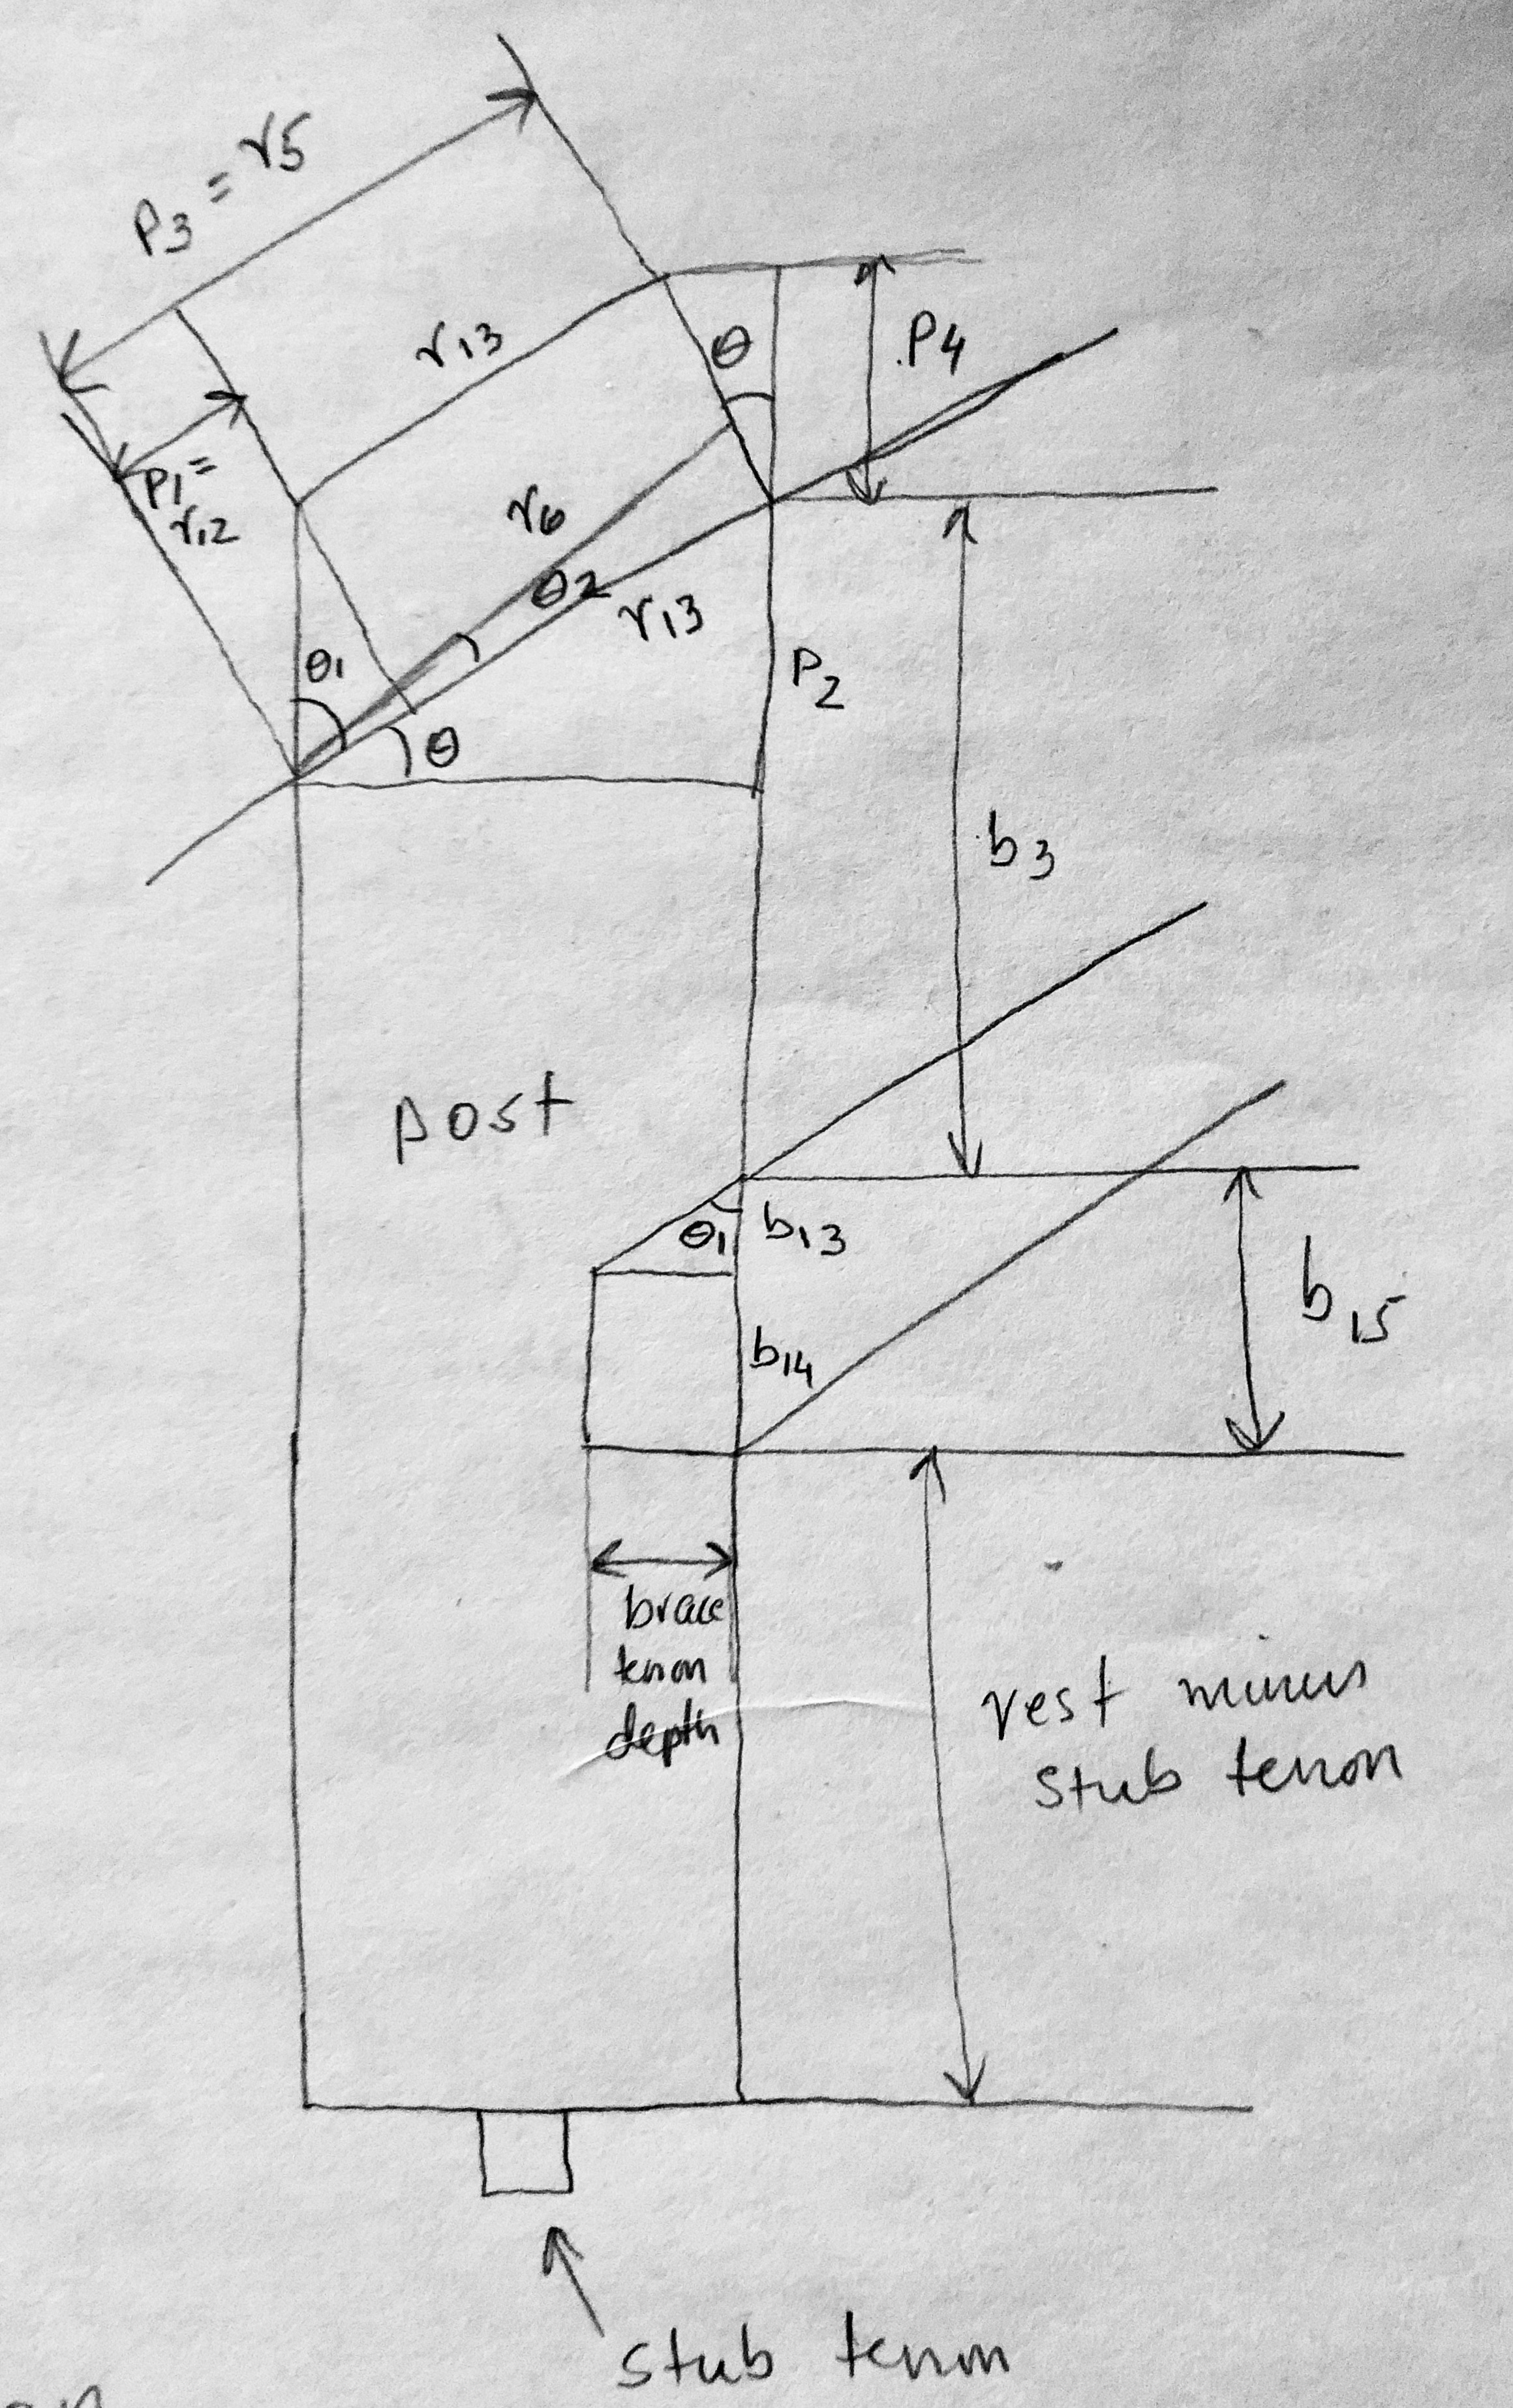
\includegraphics[width=0.4\textwidth]{images/post_calculations}
% \end{center}

Layout \& cut steps: 
\begin{enumerate}
  \item Cut a 6$\times$8 beam to 8' 2" 17/32. 
  \item Mark out 
  \begin{itemize}
    \item $p_4$ = 0' 3" 1/16
    \item $b_3$ = 1' 6" 9/16
    \item $b_{15}$ = 0' 6" 1/2, then 
    \item the rest minus stub tenon = 5' 8" 3/8, and 
    \item verify 2 inches left over for stub tenon. 
  \end{itemize}
  \item At top, cut shouldered tenon as in diagram: 
  \begin{itemize}
    \item Mark out $\theta$ = 39.8 as shown on the right side and mark out tenon depth = 4.
    \item At $90^\circ$, measure out $p_3$ = 0' 10" 13/32, and extend line from left side and verify $p_1$ = 0' 3" 11/32.
    \item Verify that straight part is $r_{13}$ = 0' 7" 3/32. 
    \item Mark out shoulder = 1 and verify that $\theta_2$ = 5.5 and $r_6$ = 0' 10" 15/32; \textbf{this is the tenon cut line}.  
    \item Create tenon at 2-in thick. 
  \end{itemize}
  \item Cut brace mortise:
    \begin{itemize}
      \item Mark out 
      \begin{itemize}
        \item $b_{13}$ = 0' 2" 1/2 and 
        \item $b_{14}$ = 0' 4" 0/2.
      \end{itemize}
      \item Drill straight at $b_{14}$ to depth of 3
      \item Angled mortise at $b_{13}$ at an angle of $\theta_1$
    \end{itemize}
  \item Cut stub tenon such that when raising, the long axis of tenon is along direction of pulling, else it could break while being raised. Perhaps the stub should be 2$\times$2$\times$2, with placement TBD. 
\end{enumerate}

\newpage
\subsection{Rafters}\label{rafter-cut-plan}

\subsubsection{Assumptions} \label{rafter-cut-plan-assumptions}

\begin{knitrout}
\definecolor{shadecolor}{rgb}{0.969, 0.969, 0.969}\color{fgcolor}\begin{kframe}
\begin{alltt}
\hlstd{rafter_width} \hlkwb{<-} \hlnum{6}
\hlstd{collar_tie_rafter_shoulder_depth} \hlkwb{<-} \hlnum{1}
\end{alltt}
\end{kframe}
\end{knitrout}

% \subsubsection{Imported variables} \label{rafter-cut-plan-imported-variables}
% 
% \begin{itemize}
%   \item \verb+rafter_height+ = rafter_height (\Cref{kp-collar-tie-assumptions}).
%   \item \verb+x8+ = x8 from \Cref{posts-rafters-calculations}
%   \item \verb+h6+ = h6 from \Cref{posts-rafters-calculations}
%   \item \verb+r7+ = r7 from \Cref{rafter-lengths-connections-calculations}
%   \item \verb+r5+ = r5 from \Cref{rafter-lengths-connections-calculations}
%   \item \verb+r4+ = r4 from \Cref{rafter-lengths-connections-calculations}
%   \item \verb+r3+ = r3 from \Cref{rafter-lengths-connections-calculations}
%   \item \verb+r2+ = r2 from \Cref{rafter-lengths-connections-calculations}
%   \item \verb+rafter_length_final+ = rafter_length_final from \Cref{kp-rafter-joints-calculations}
%   \item \verb+k14_imperial+ = k14_imperial from \Cref{kp-rafter-joints-calculations}
%   \item \verb+post_rafter_shoulder_depth+ = post_rafter_shoulder_depth from \Cref{rafter-lengths-connections-assumptions}
%   \item \verb+rafter_length_final_imperial+ = rafter_length_final_imperial from \Cref{kp-rafter-joints-calculations}
%   \item \verb+theta2_degrees+ = theta2_degrees from \Cref{rafter-lengths-connections-calculations}
%   \item \verb+theta3_degrees+ = theta3_degrees from \Cref{rafter-lengths-connections-calculations}
% \end{itemize}






\subsubsection{Rafter overall}
\begin{figure}[h]       
    \fbox{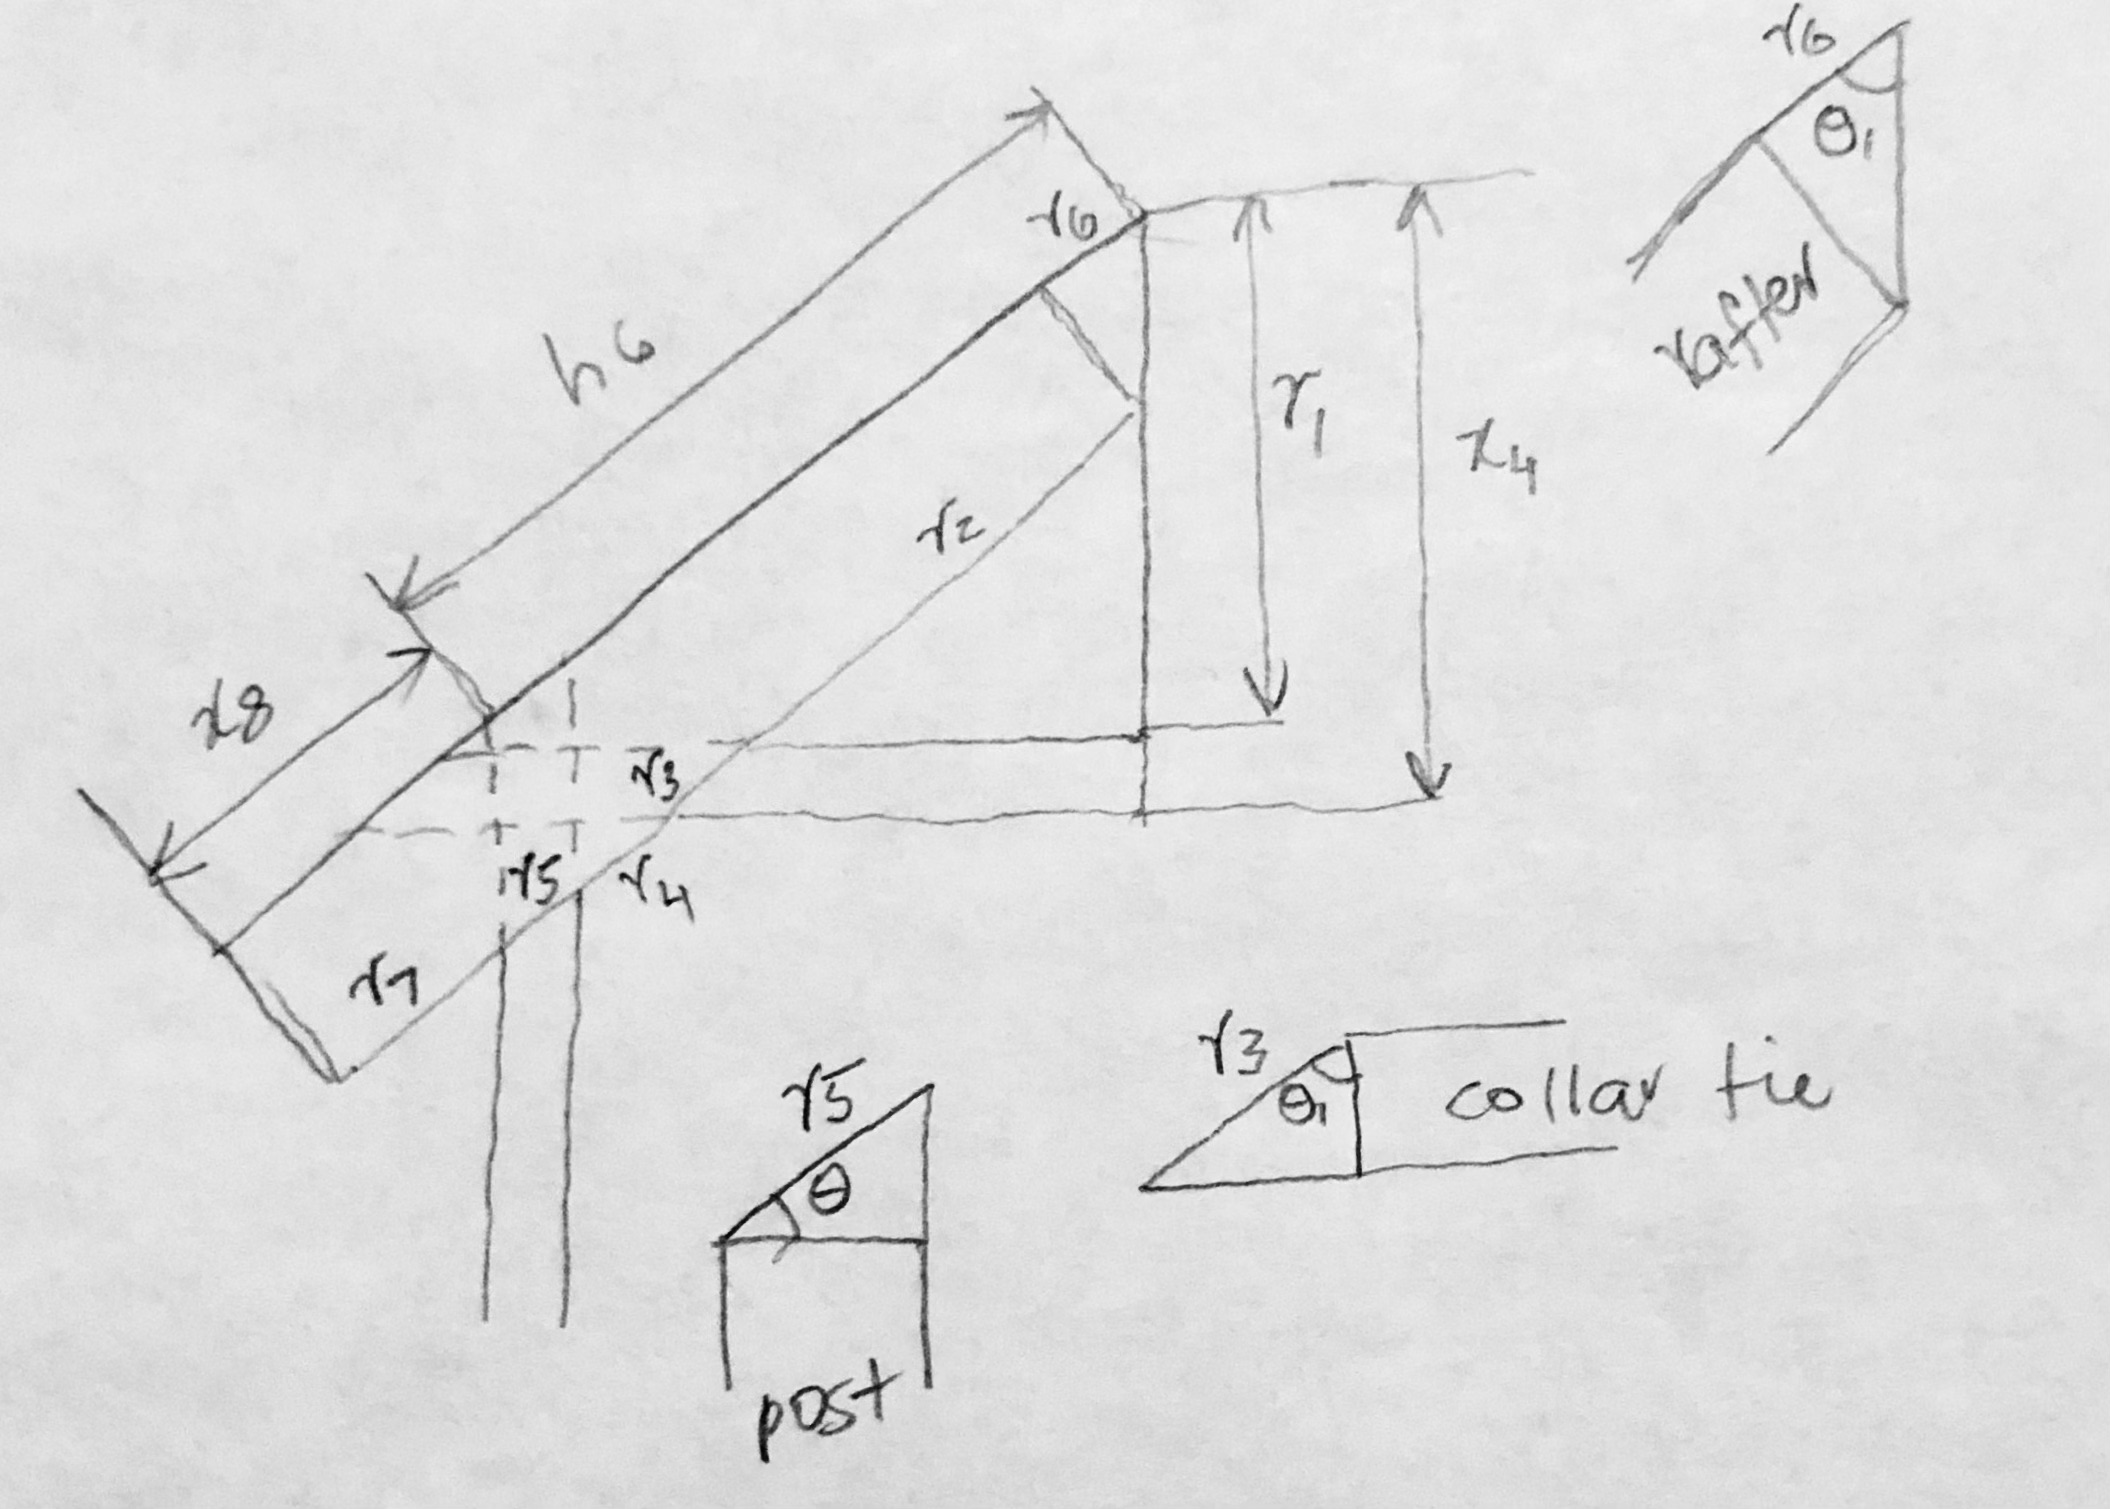
\includegraphics[width=0.45\textwidth]{images/rafter_length}}   
    \hspace{30px}
    \fbox{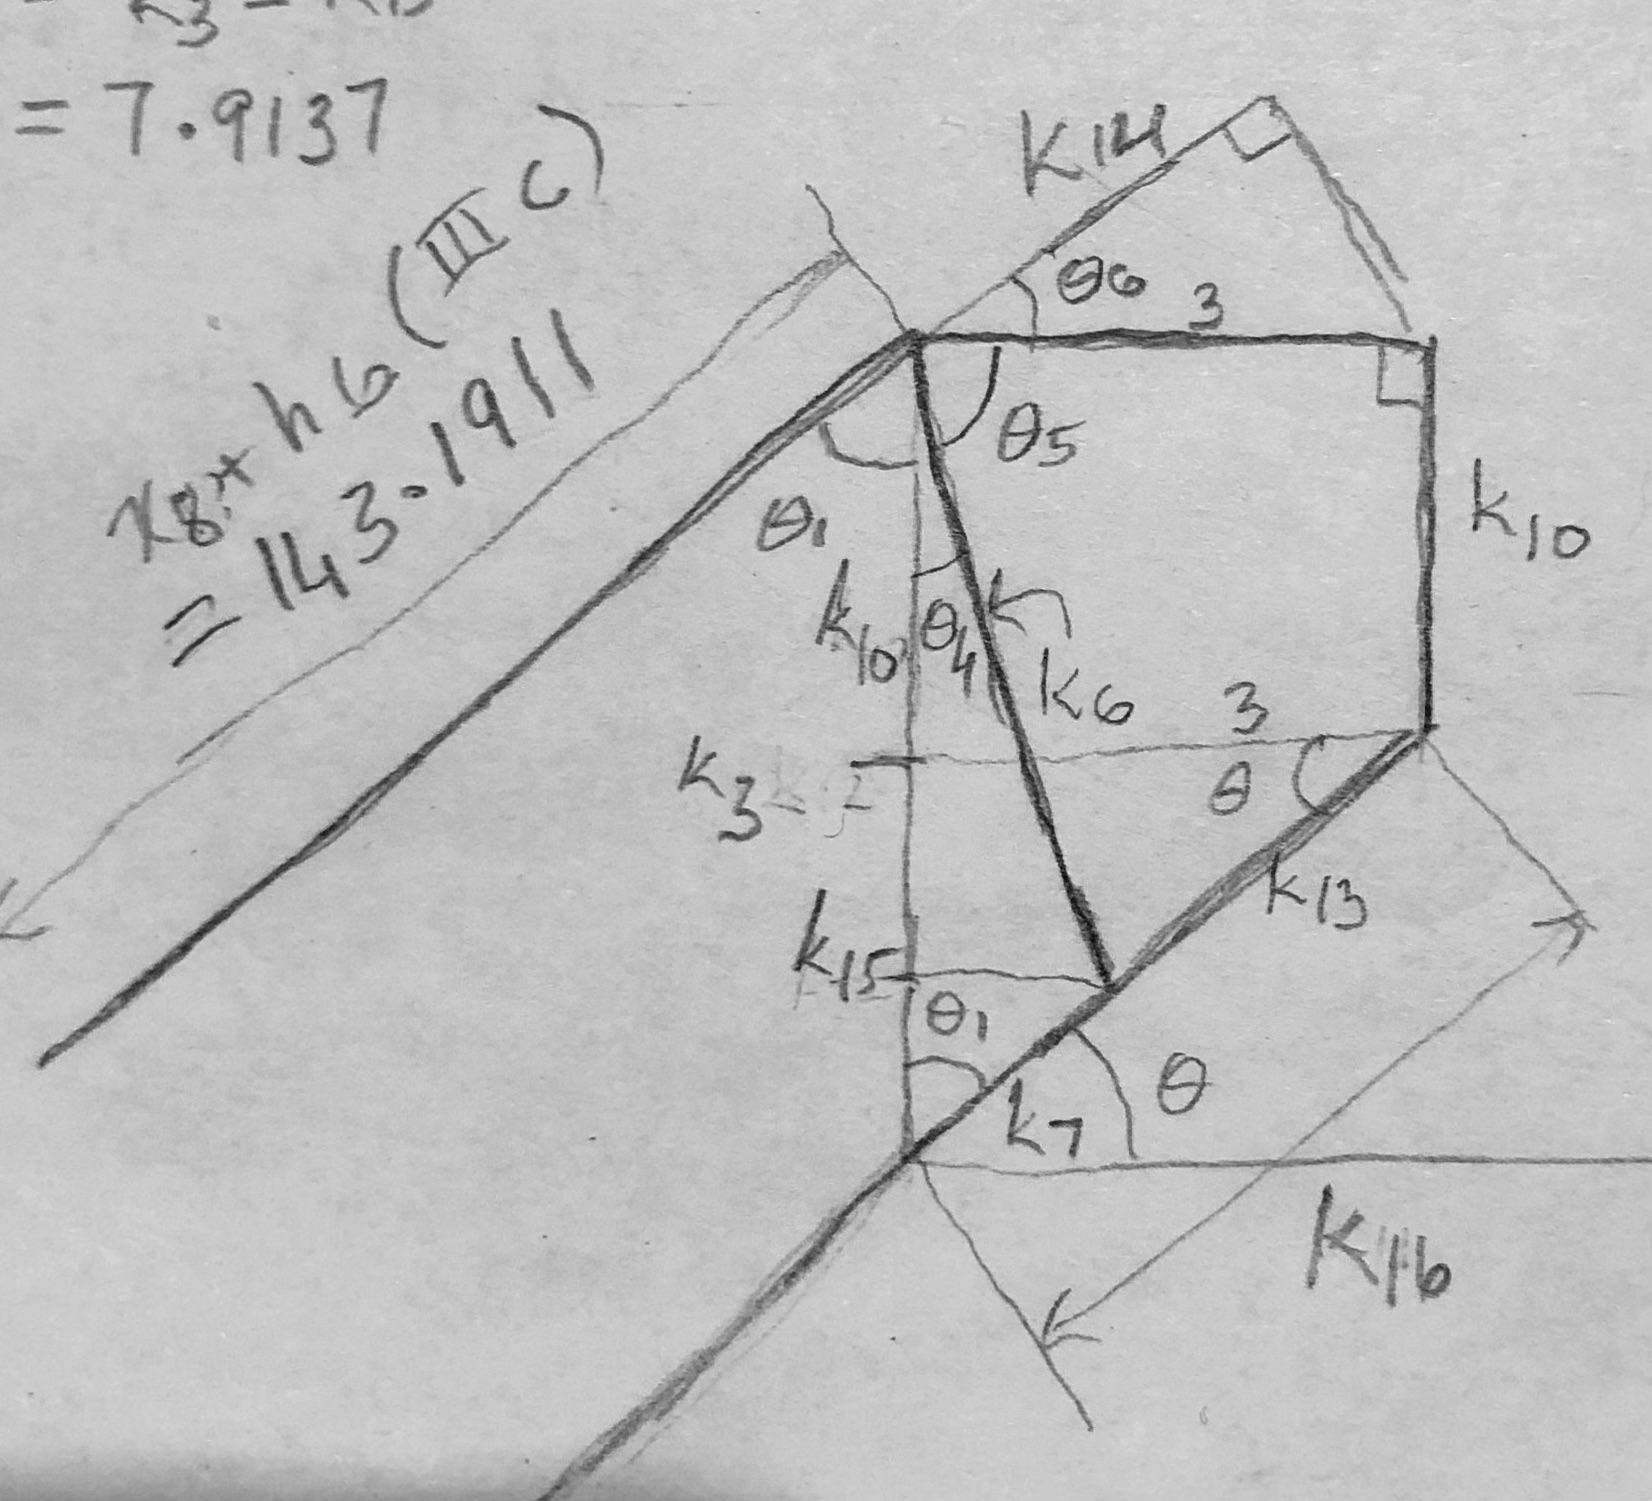
\includegraphics[width=0.36\textwidth]{images/rafter_tenon_detail}}
    \caption{Rafter marks}
\end{figure}

\begin{enumerate}
  \item Measure out 6$\times$8$\times$\text{12' 1" 1/2}.
  \item On top side mark out (left to right) $x_8 = $ 2' 7" 1/4 and $h_6 = $ 9' 3" 15/16. Verify that $k_{14}$ = 0' 2" 5/16. 
  \item On the bottom, mark out (left to right) the following:
  \begin{align*}
    r_7 &= 2' 0" 9/16\\
    r_5 &= 0' 10" 13/32\\
    r_4 &= \text{0' 5" 27/32}\\
    r_3 &= 1' 0" 1/2\\
    r_2 &= 6' 11" 3/16\\
    & \text{and verify that what's left over} = \text{0' 8" 31/32}.
  \end{align*}
\end{enumerate}



\subsubsection{Mortise for post tenon}

\begin{center}
	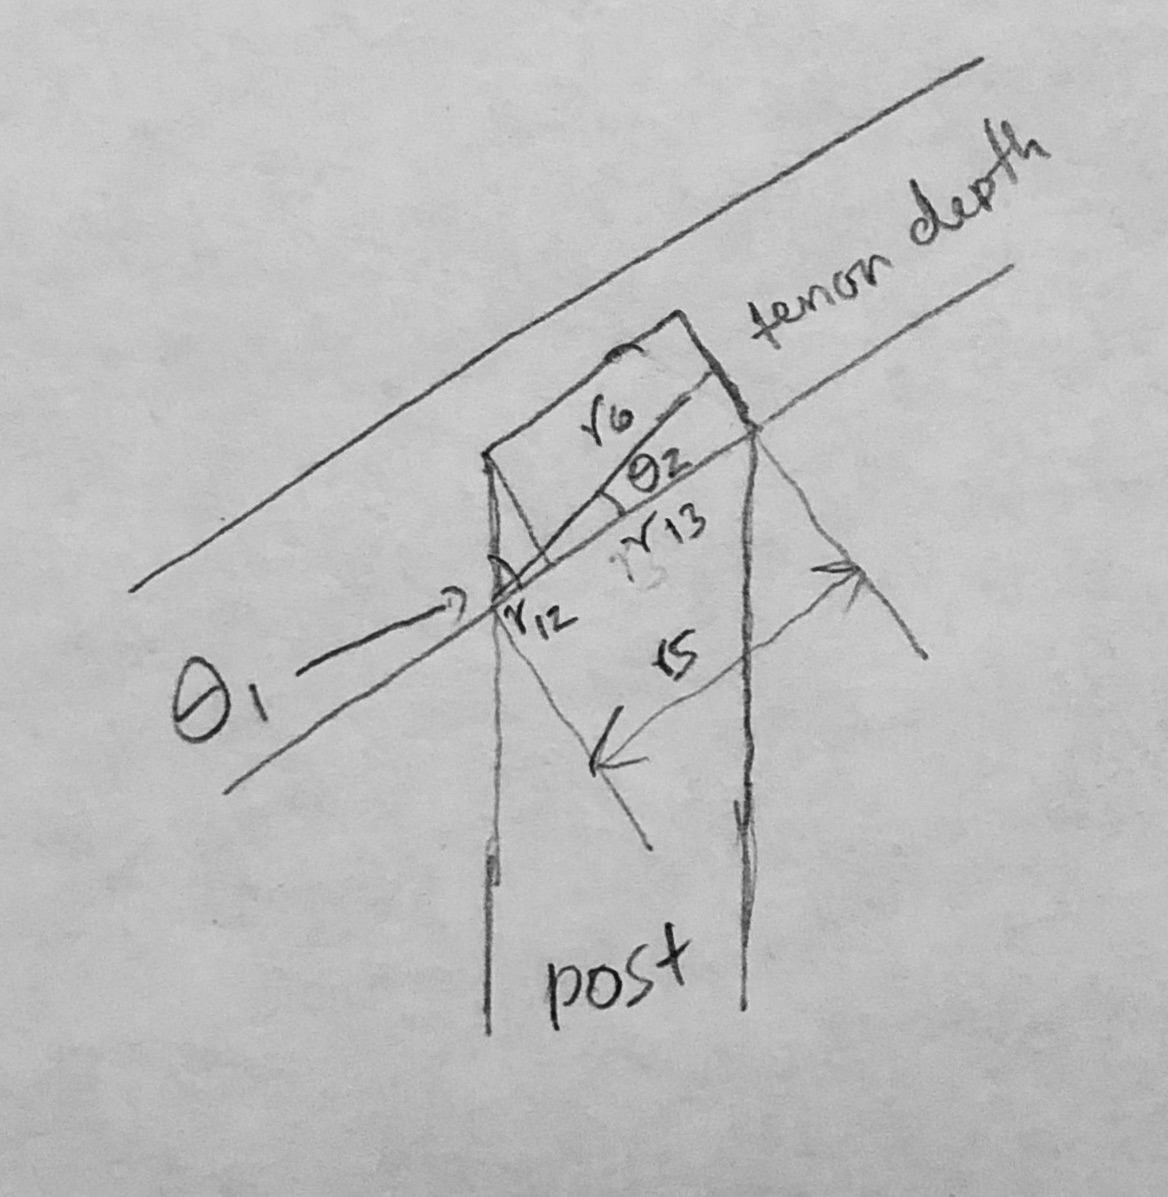
\includegraphics[width=0.5\textwidth]{images/post_tenons_into_rafters}
\end{center}

At $r_5$, mark out 1-in shoulder, verify that $\theta_2$ = 5.5 and all other variables in diagram.

\subsubsection{Mortise for collar tie tenon}

\begin{center}
	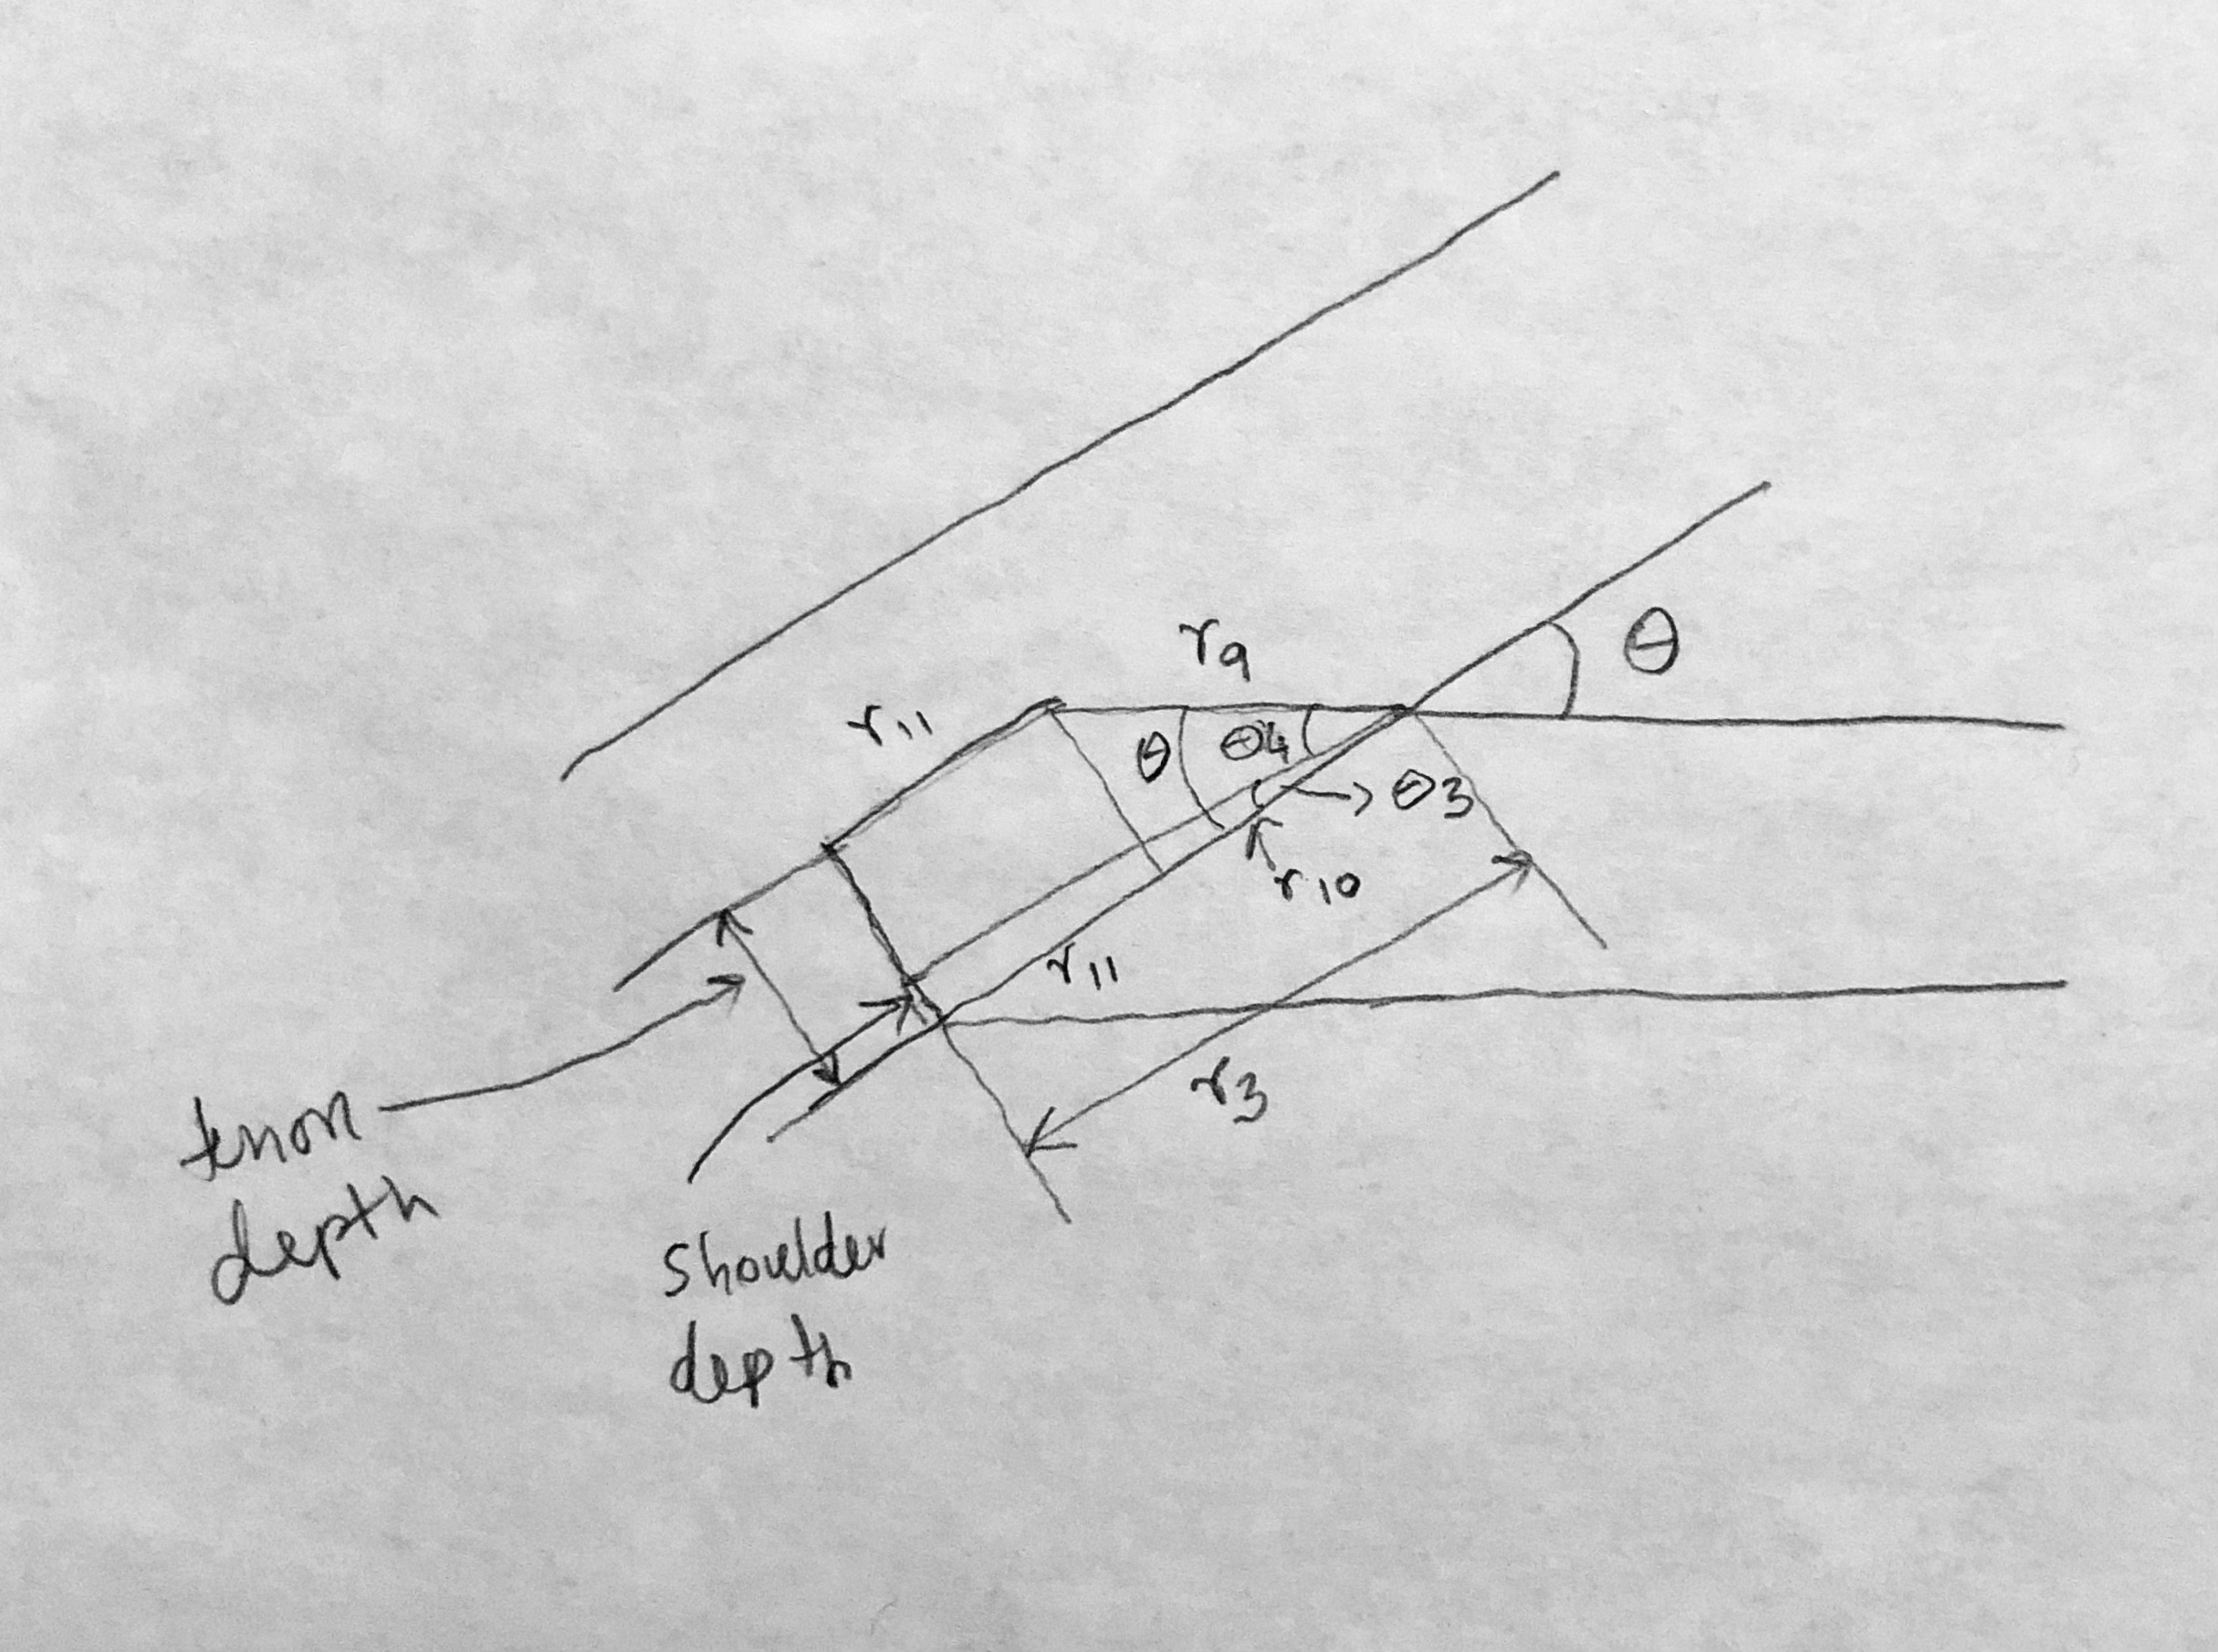
\includegraphics[width=0.5\textwidth]{images/collar_tie_tenons_into_rafters}
\end{center}

At $r_3$, mark out 1-in shoulder and verify that $\theta_3$ = 4.6 and all other variables in diagram. 

\subsubsection{Mortise for strut tenon}

\begin{center}
	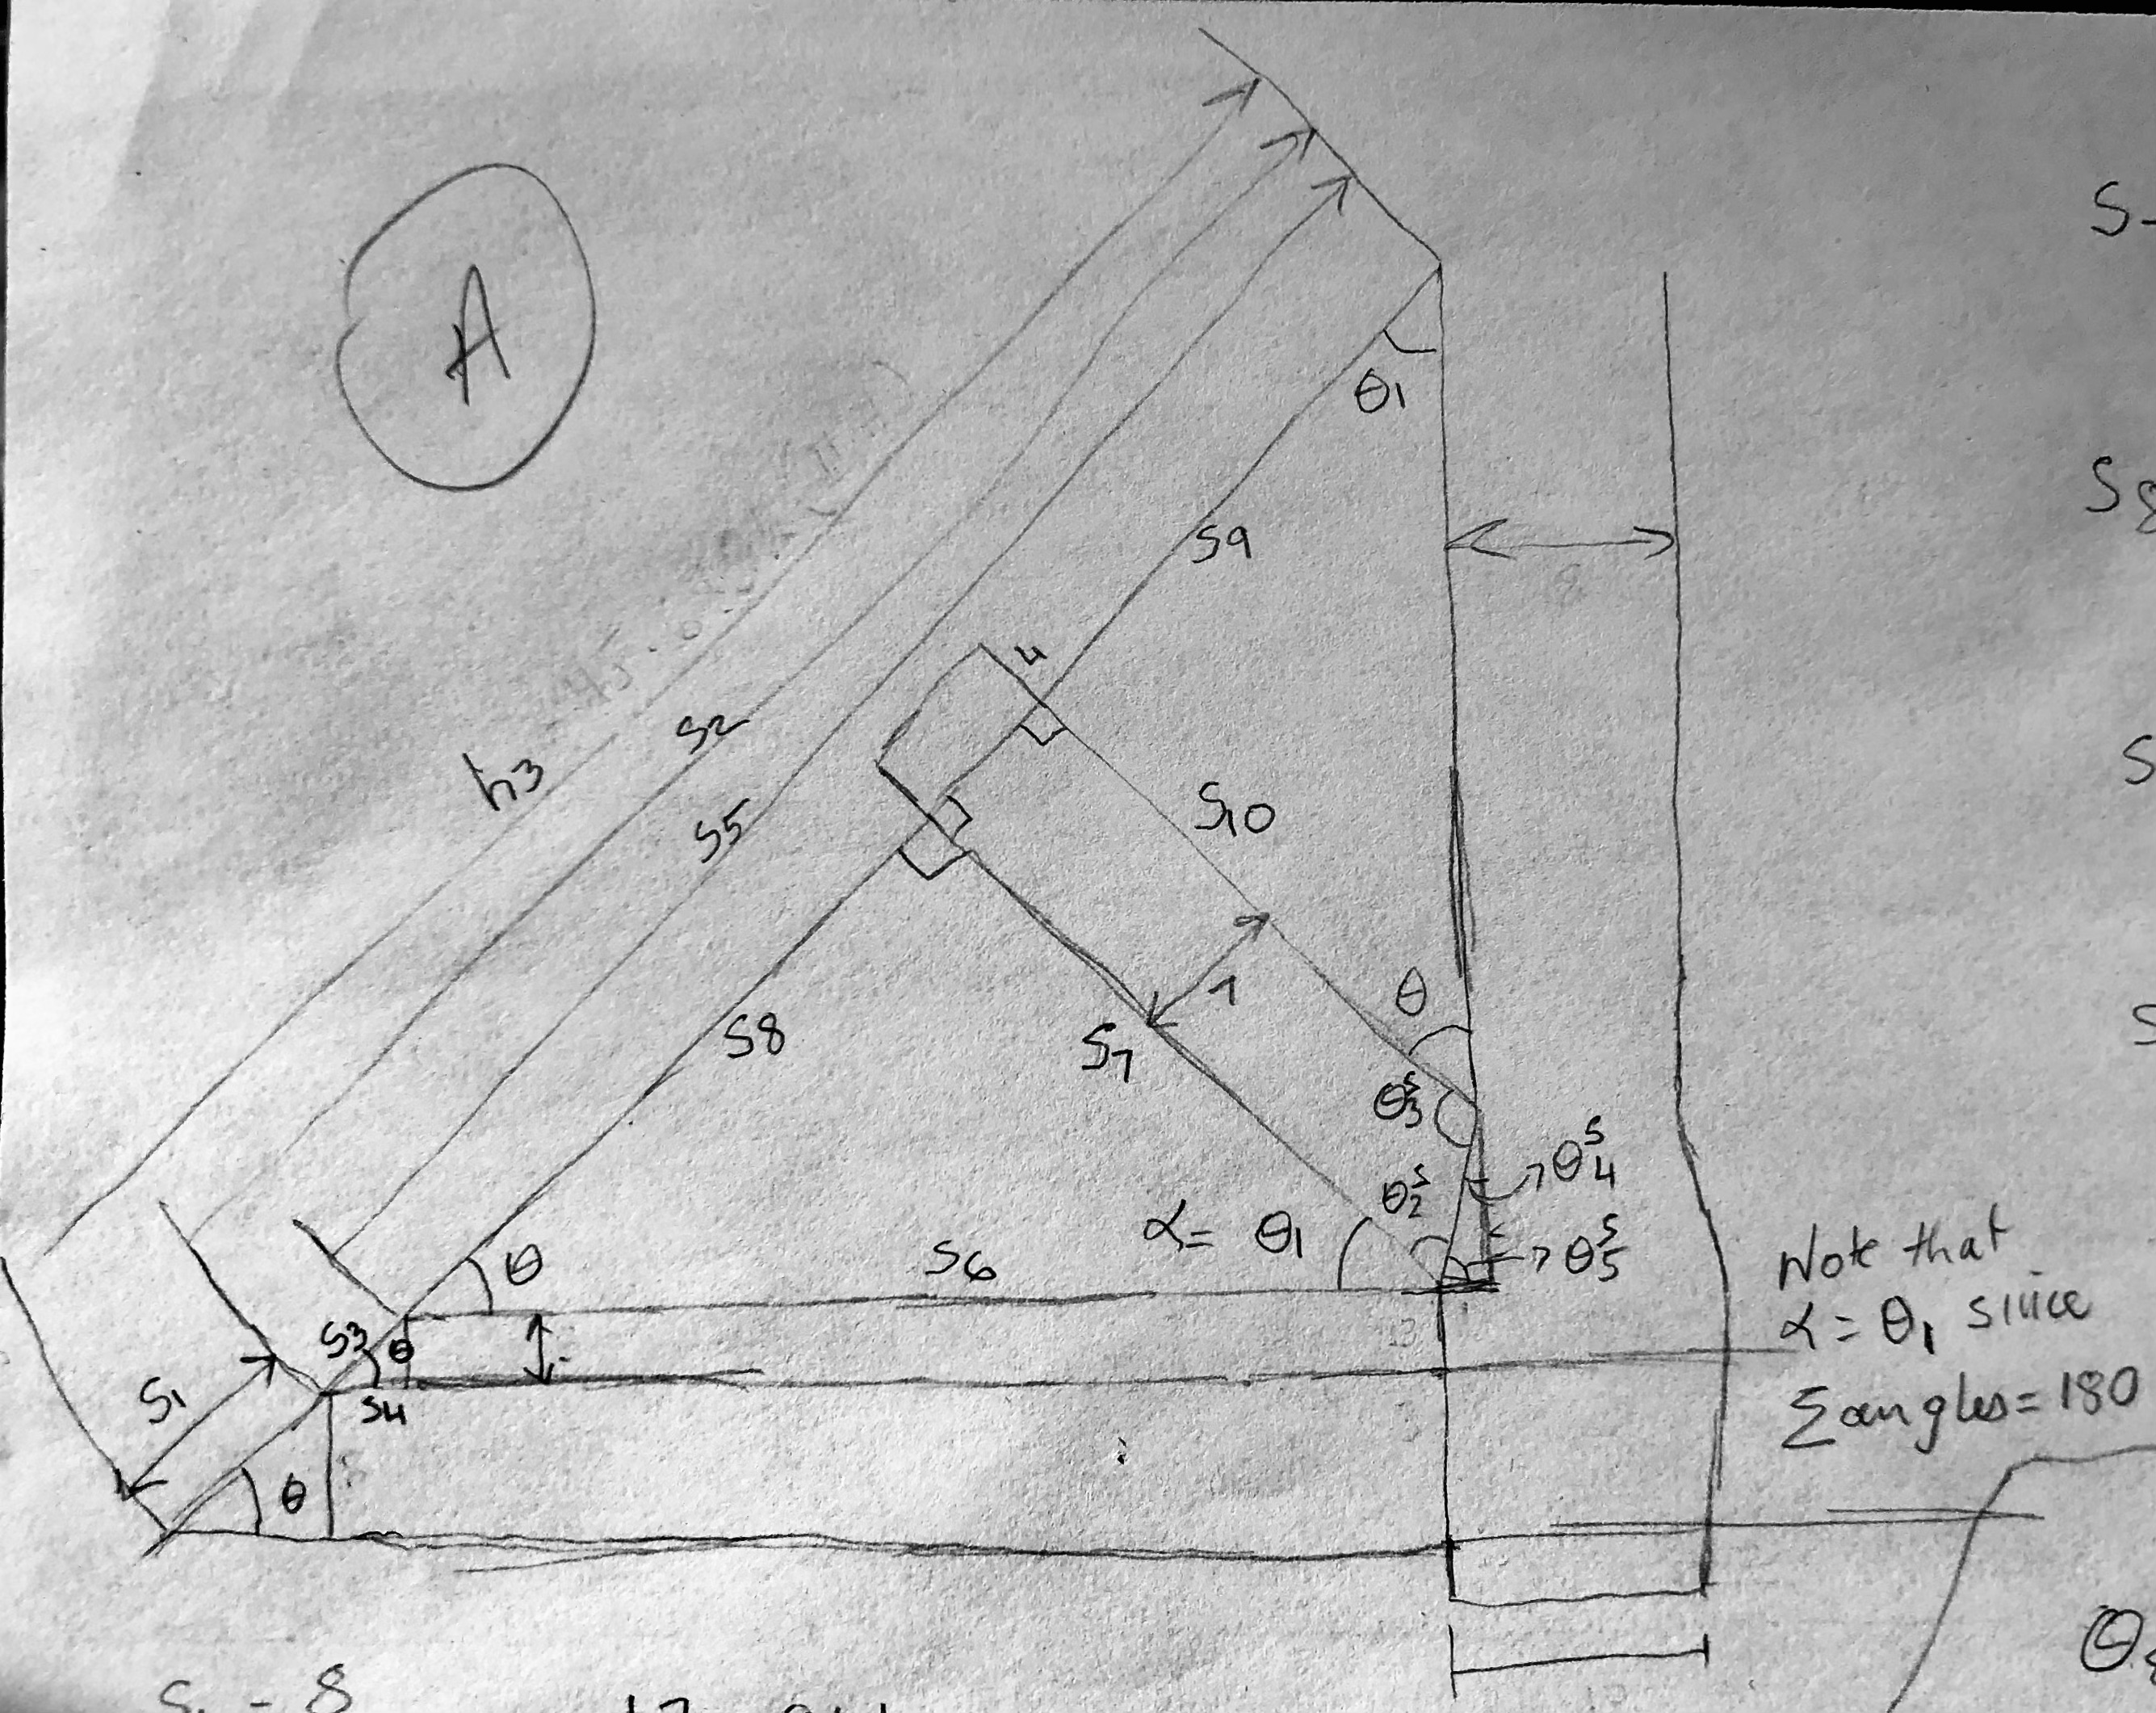
\includegraphics[width=0.5\textwidth]{images/strut_kp_overall}
\end{center}

For strut mortises into rafter, measure $s_3 + s_8$ from end of collar tie mortise (sans shoulder), which is 
\[ s_3 + s_8 = 50.2444 = 4' 2" 1/4.\]

Mortise/tenon is 1.5-in thick, 5-in wide, and 4-in deep. Verify that $s_9$ = 2' 3" 15/16. 

\subsubsection{Tenon for KP mortise}

  \begin{center}
	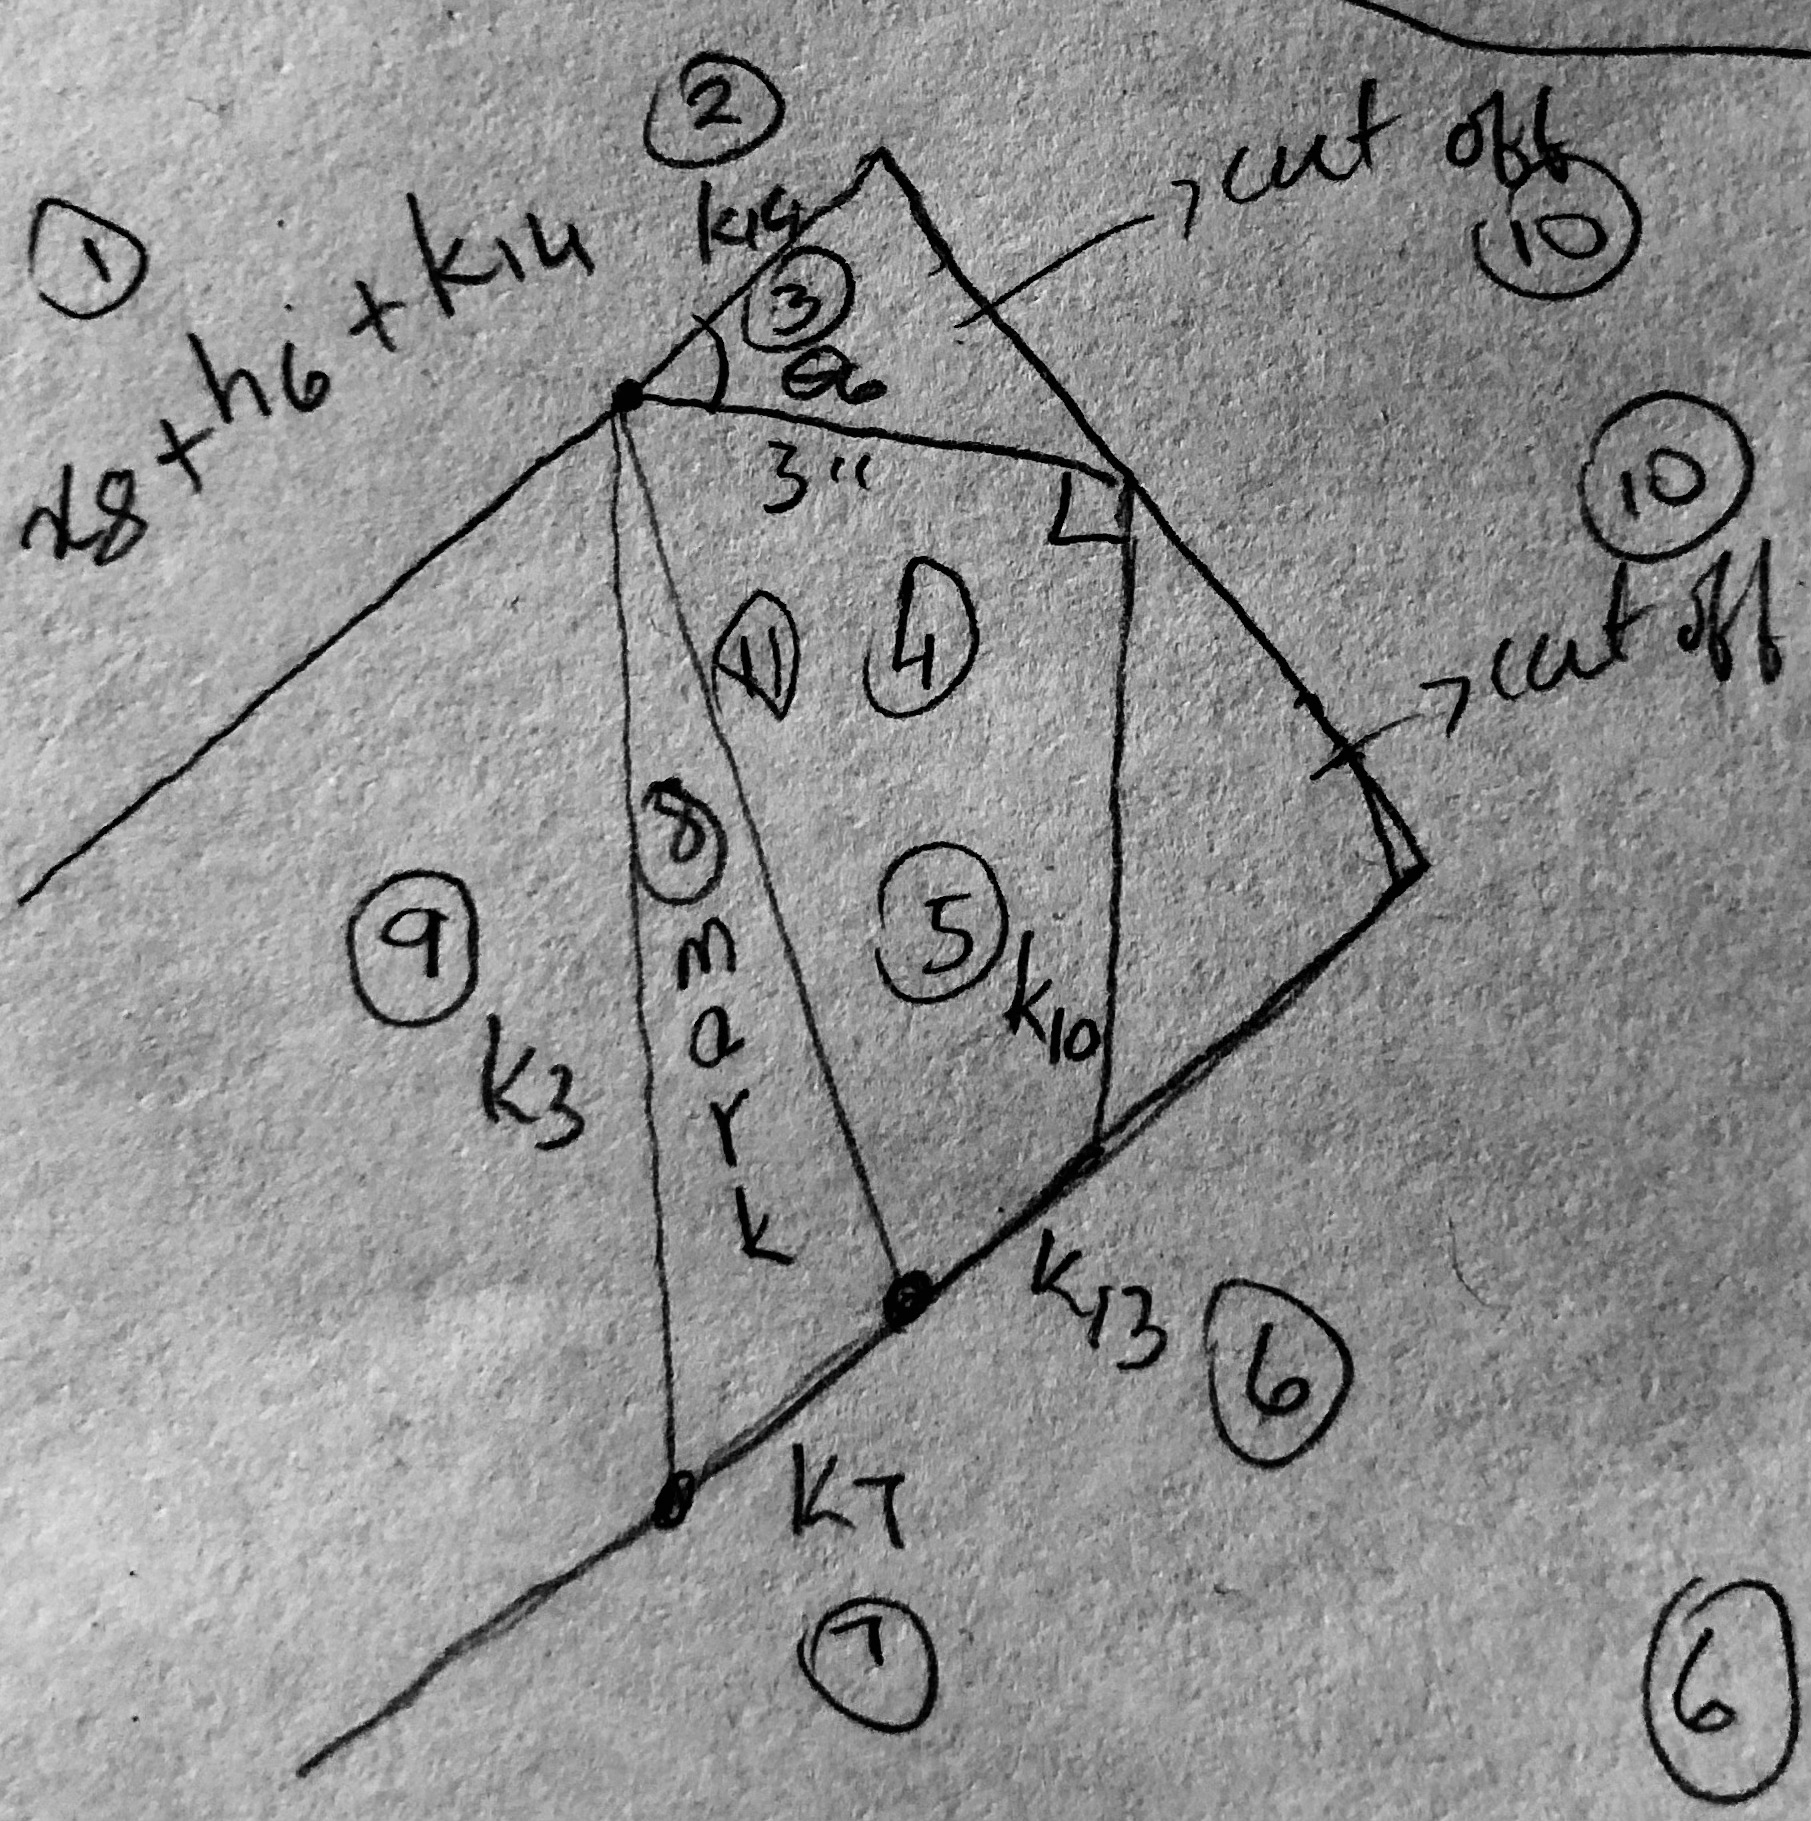
\includegraphics[width=0.4\textwidth]{images/rafter_layout}
\end{center}
Numbers below correspond to diagram. \textbf{There are 11 steps. The diagram hardcodes 3", ignore that.}

\vspace{0.25cm}

\begin{enumerate}
  \item $k_{14}$ = \text{0' 2" 5/16} should have been marked out already. 
  \item Mark out $\theta_6$ = 39.8 and verify rafter tenon depth into KP (\text{0' 3"}).
  \item Mark $90^\circ$ (\textbf{this angle is hardcoded as 90}).
  \item Verify $k_{10} = $  \text{0' 7" 29/32}.
  \item Measure $k_{13} = $ \text{0' 2" 19/32}.
  \item Measure $k_7 = $ \text{0' 1" 5/16}.
  \item Mark up to $k_{14}$ point.
  \item Verify $k_3 = $ \text{0' 10" 13/32}.
  \item Cut off sections.
  \item Create tenons at 2-in thick. 
\end{enumerate}


\textbf{TODO rafters will house purlins - account for those also when purlin nos is finalized.}


\newpage

\subsection{Kingpost}\label{kp-layout-and-cuts}
\subsubsection{Assumptions}
\begin{knitrout}
\definecolor{shadecolor}{rgb}{0.969, 0.969, 0.969}\color{fgcolor}\begin{kframe}
\begin{alltt}
\hlstd{kp_depth} \hlkwb{<-} \hlnum{6}
\hlstd{kp_top_tenon_thickness} \hlkwb{<-} \hlnum{1.5}
\end{alltt}
\end{kframe}
\end{knitrout}

% \subsubsection{Imported variables}
% 
% 
% \begin{itemize}
%   \item \verb+k4+ = k4 from \Cref{kp-rafter-joints-calculations}
%   \item \verb+k3+ = k3 from \Cref{kp-rafter-joints-calculations}
%   \item \verb+strut_height_above_collar_tie+ = strut_height_above_collar_tie from \Cref{strut-kp-connections-assumptions}
%   \item \verb+kp_top_tenon_length+ = kp_top_tenon_length from \Cref{kp-collar-tie-assumptions}
%   \item \verb+kp_part+ = kp_part from \Cref{ridge-shape-and-dimensions-assumptions}
%   \item \verb+collar_tie_height+ = collar_tie_height from \Cref{kp-collar-tie-assumptions}
%   \item \verb+kp_through_tenon_length+ = kp_through_tenon_length from \Cref{kp-collar-tie-assumptions}
%   \item \verb+kp_flare+ = kp_flare from \Cref{strut-kp-connections-assumptions}
%   \item \verb+kp_rafter_shoulder_depth+ = kp_rafter_shoulder_depth from \Cref{kp-rafter-joints-assumptions}
%   \item \verb+kp_total_height_imperial+ = kp_total_height_imperial from \Cref{kp-collar-tie-calculations}
%   \item \verb+kp_width_bottom+ = kp_width_bottom from \Cref{strut-kp-connections-assumptions}
%   \item \verb+rafter_tenon_thickness+ = rafter_tenon_thickness from \Cref{kp-rafter-joints-assumptions}
%   \item \verb+strut_tenon_into_kp_depth+ = strut_tenon_into_kp_depth from \Cref{strut-kp-connections-assumptions}
%   \item \verb+strut_tenon_into_kp_thickness+ = strut_tenon_into_kp_thickness from \Cref{strut-kp-connections-assumptions}
% \end{itemize}




\begin{center}\fbox{The diagrams have some hardcoded values - ignore those.}\end{center}

\begin{figure}[h]
    \fbox{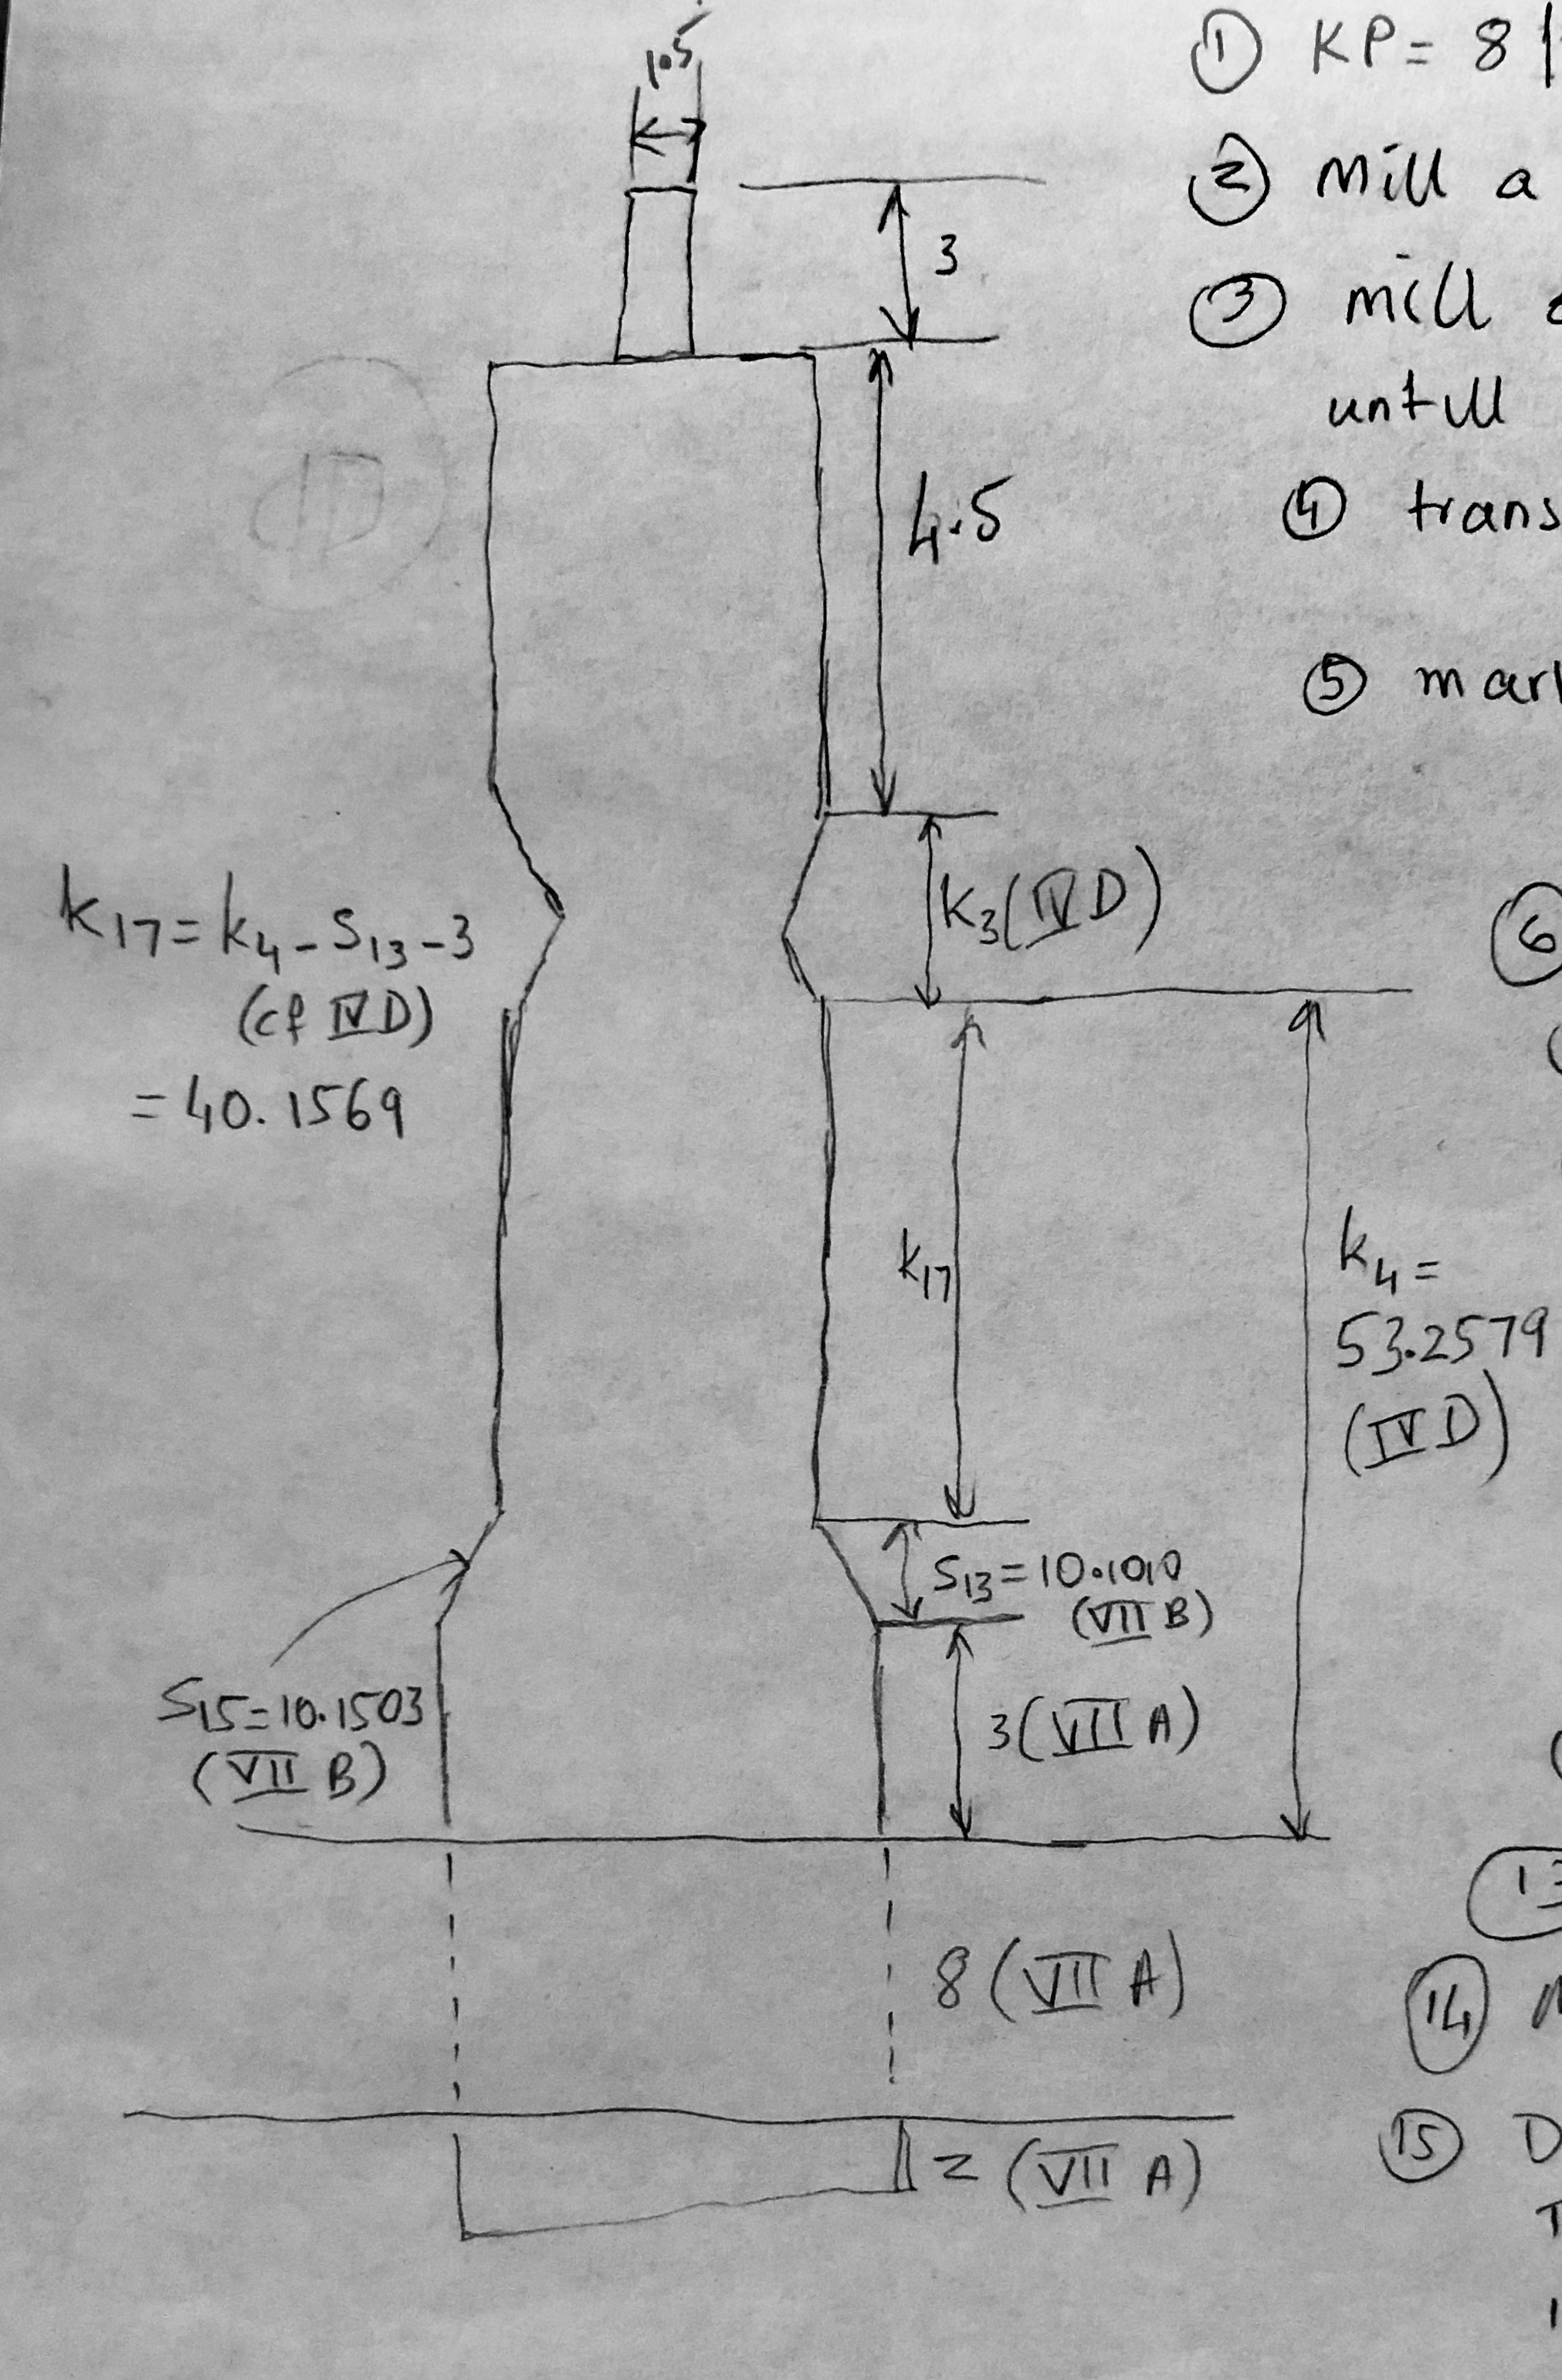
\includegraphics[width=0.45\textwidth]{images/kp_layout_and_cuts}}   
    \hspace{30px}
    \fbox{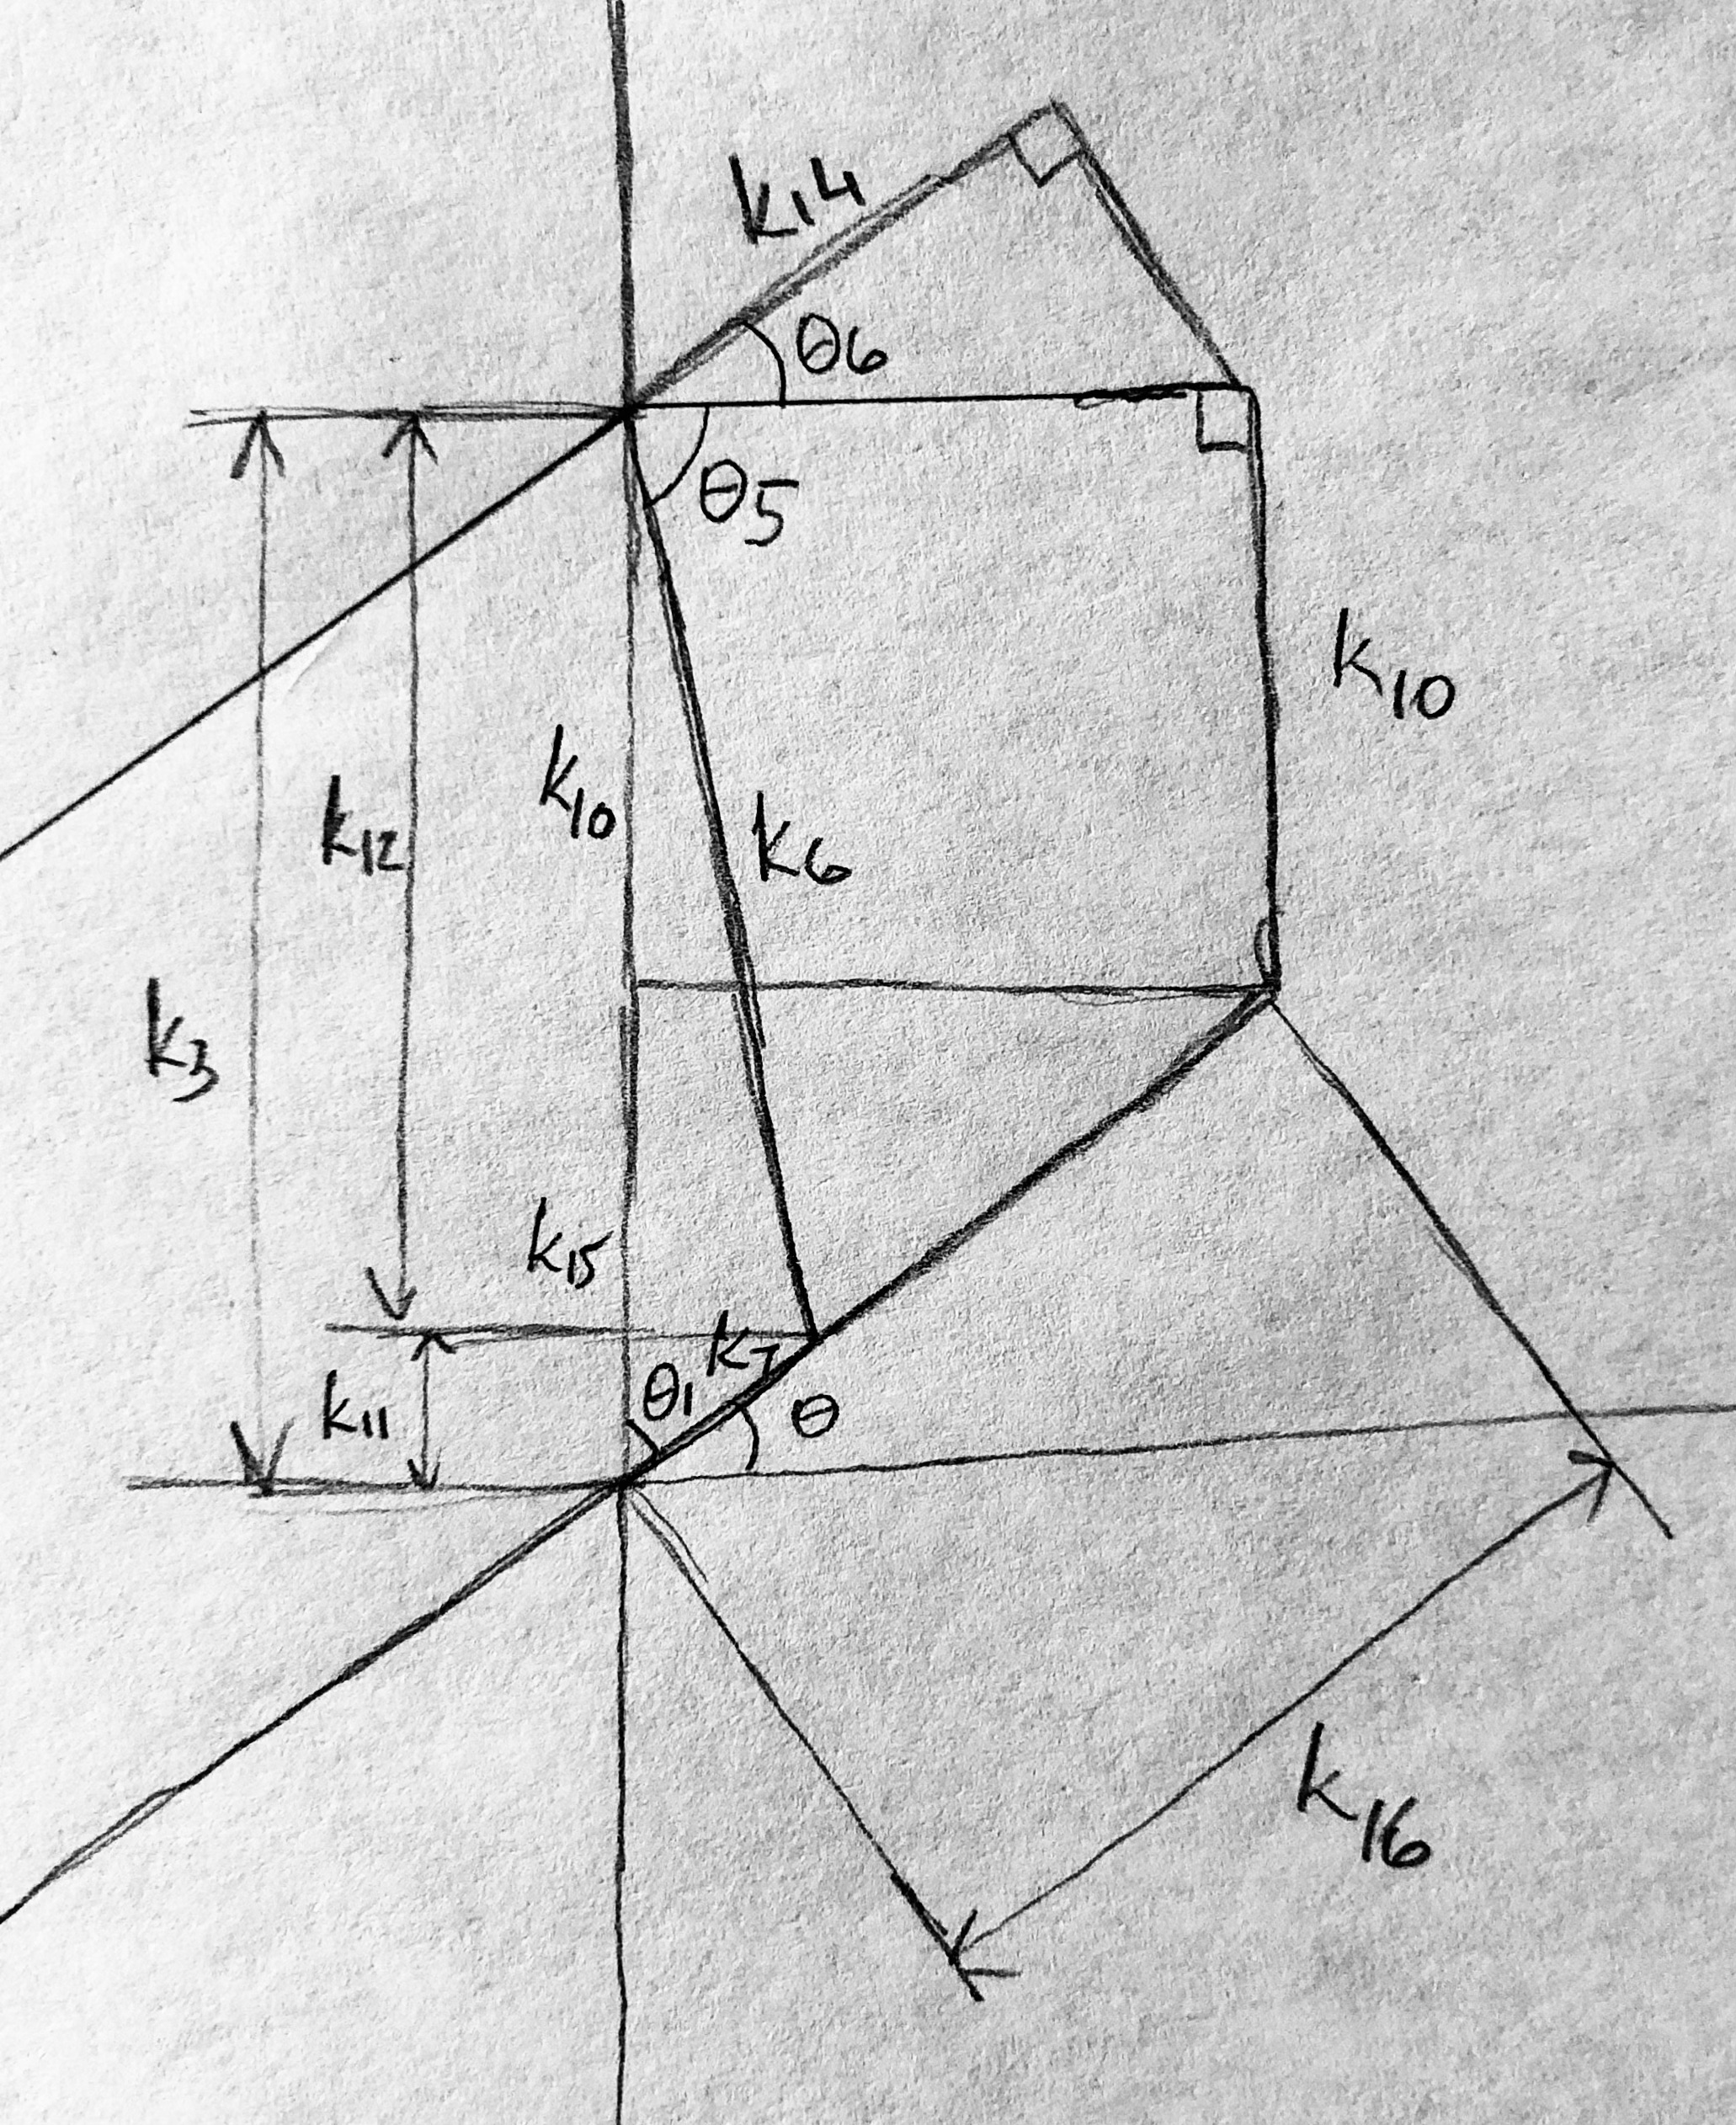
\includegraphics[width=0.4\textwidth]{images/kp_mortise_for_rafter}}
    \caption{Overall cuts + mortise for rafter}
\end{figure}


\begin{enumerate}
  \item KP total length = 6' 9" 5/32.
  \item Mill a 6$\times$10, with length as above. 
  \item Mill off 1 inch on both sides, from top until 61.1898 = 5' 1" 3/16. 
  \item Transitional area = $s_{13}$ = 0' 6" 31/32; chisel or saw this out, and verify that $s_{15}$ = 0' 7" 1/16.
  \item Mark out from top: KP top tenon length = 3, KP part = 4.5, $k_3$ = 0' 10" 13/32, verify that $k_{17}$ = 3' 7" 9/32. Mark $s_{13}$ = 0' 6" 31/32, strut height above collar tie = 3, and collar tie height = 8, and finally, through tenon length = 2.
  \item Cut top tenon at thickness = 1.5 and length 3.
  \item Cut bottom tenon at 10 inches long.
  \item At $k_3$ mortise, mark out $k_{11}$ = 0' 0" 27/32 and $k_{12}$ = 0' 9" 19/32. 
  \item Mark out 1 inch shoulder down the sides. 
  \item Mark $k_{10}$ = 0' 7" 29/32 and $k_{15}$ = 0' 2" 1/2. 
  \item Drill straight at $k_{10}$, 2-inch mortise and create angled mortise at $k_{15}$. 
  \item Create shoulder using $k_{11}$ and $k_{12}$ measurements above. 
  \item For strut mortises, verify $s_{15}$ = 0' 7" 1/16.
  \item Mark out $s_{16}$ = 0' 1" 13/16 and $s_{17}$ = 0' 5" 1/4. Note that $s_{15} = s_{16} + s_{17}$. 
  \item Drill 1.5-inch thick mortises at $90^\circ$ along $s_{17}$ and angled along $s_{16}$. Mortises are 2 inches deep. Use some sort of right-angle guide for the drill since the face being drilled into is at an angle. 
\end{enumerate}

\begin{figure}[h]
    \fbox{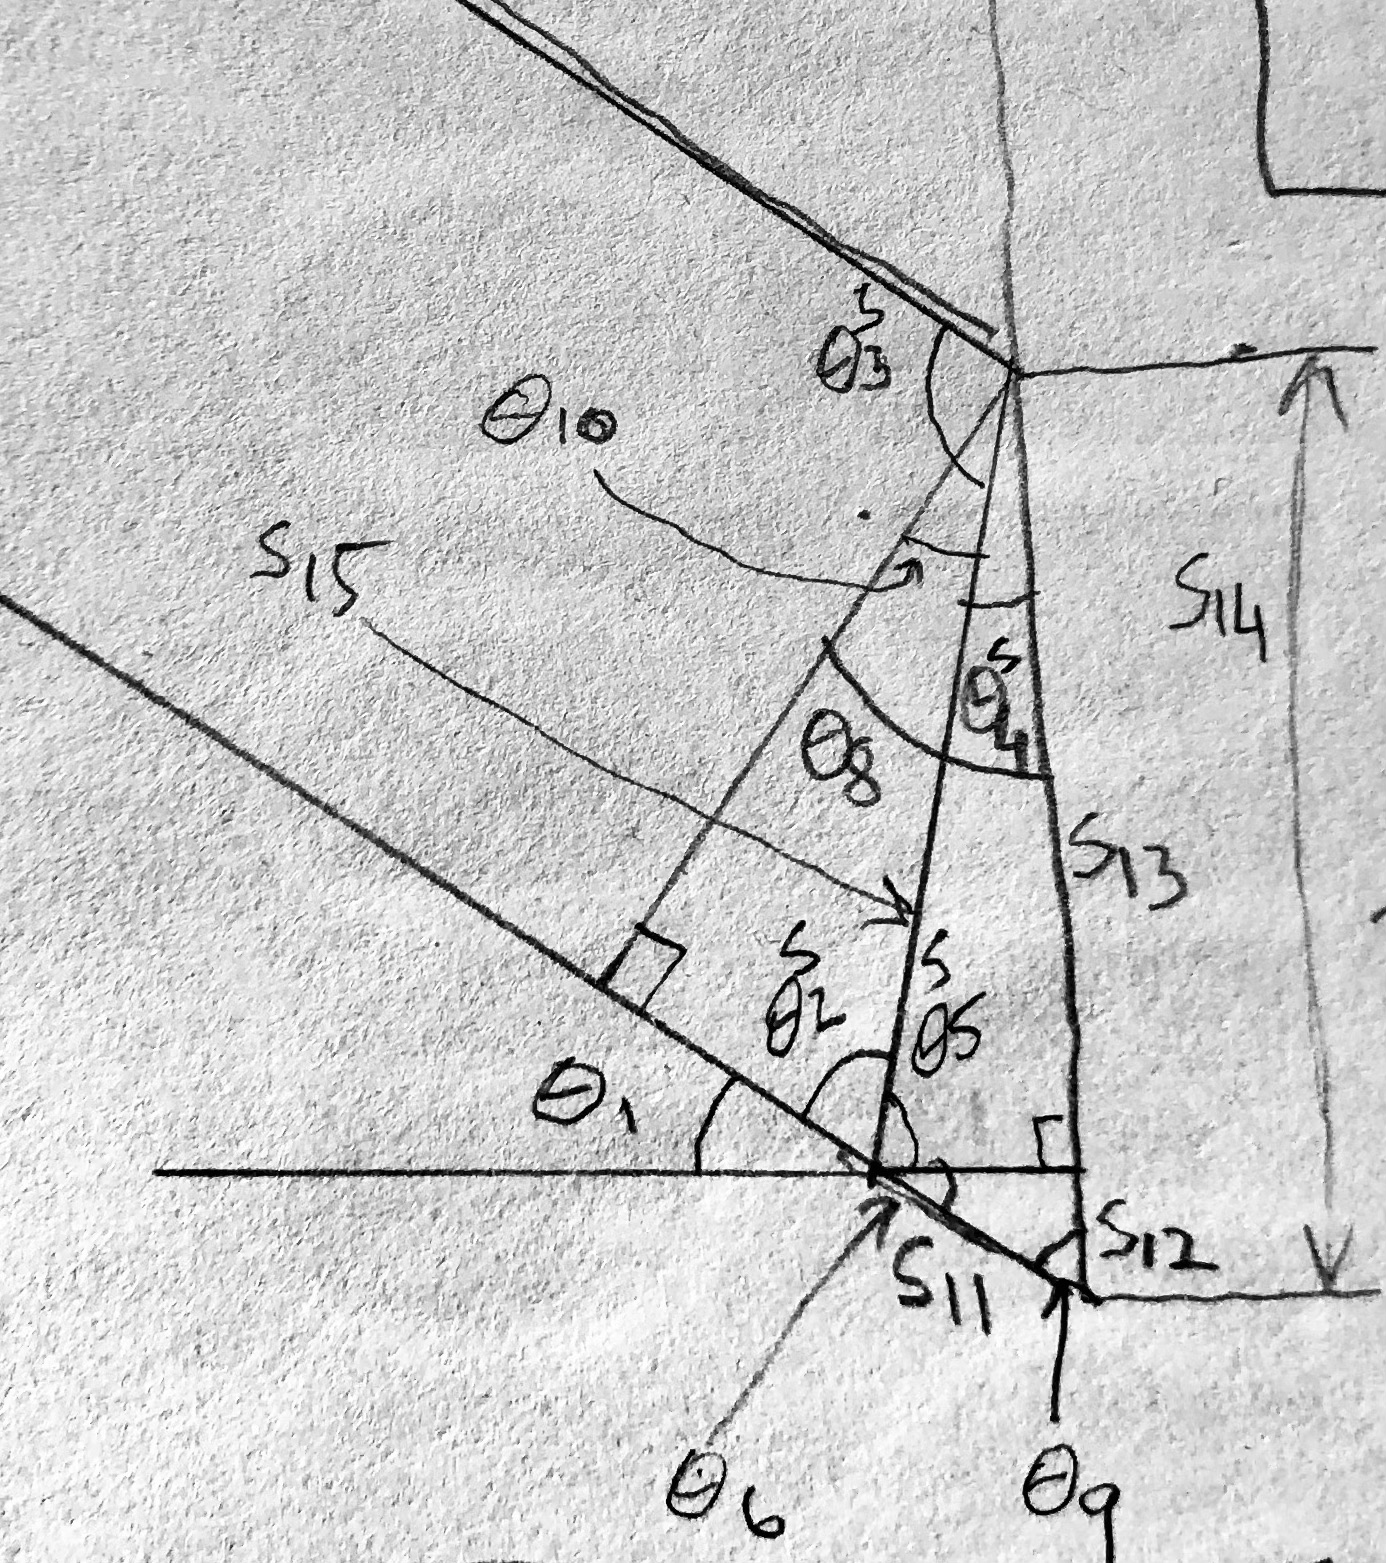
\includegraphics[width=0.45\textwidth]{images/strut_kp_detail}}   
    \hspace{30px}
    \fbox{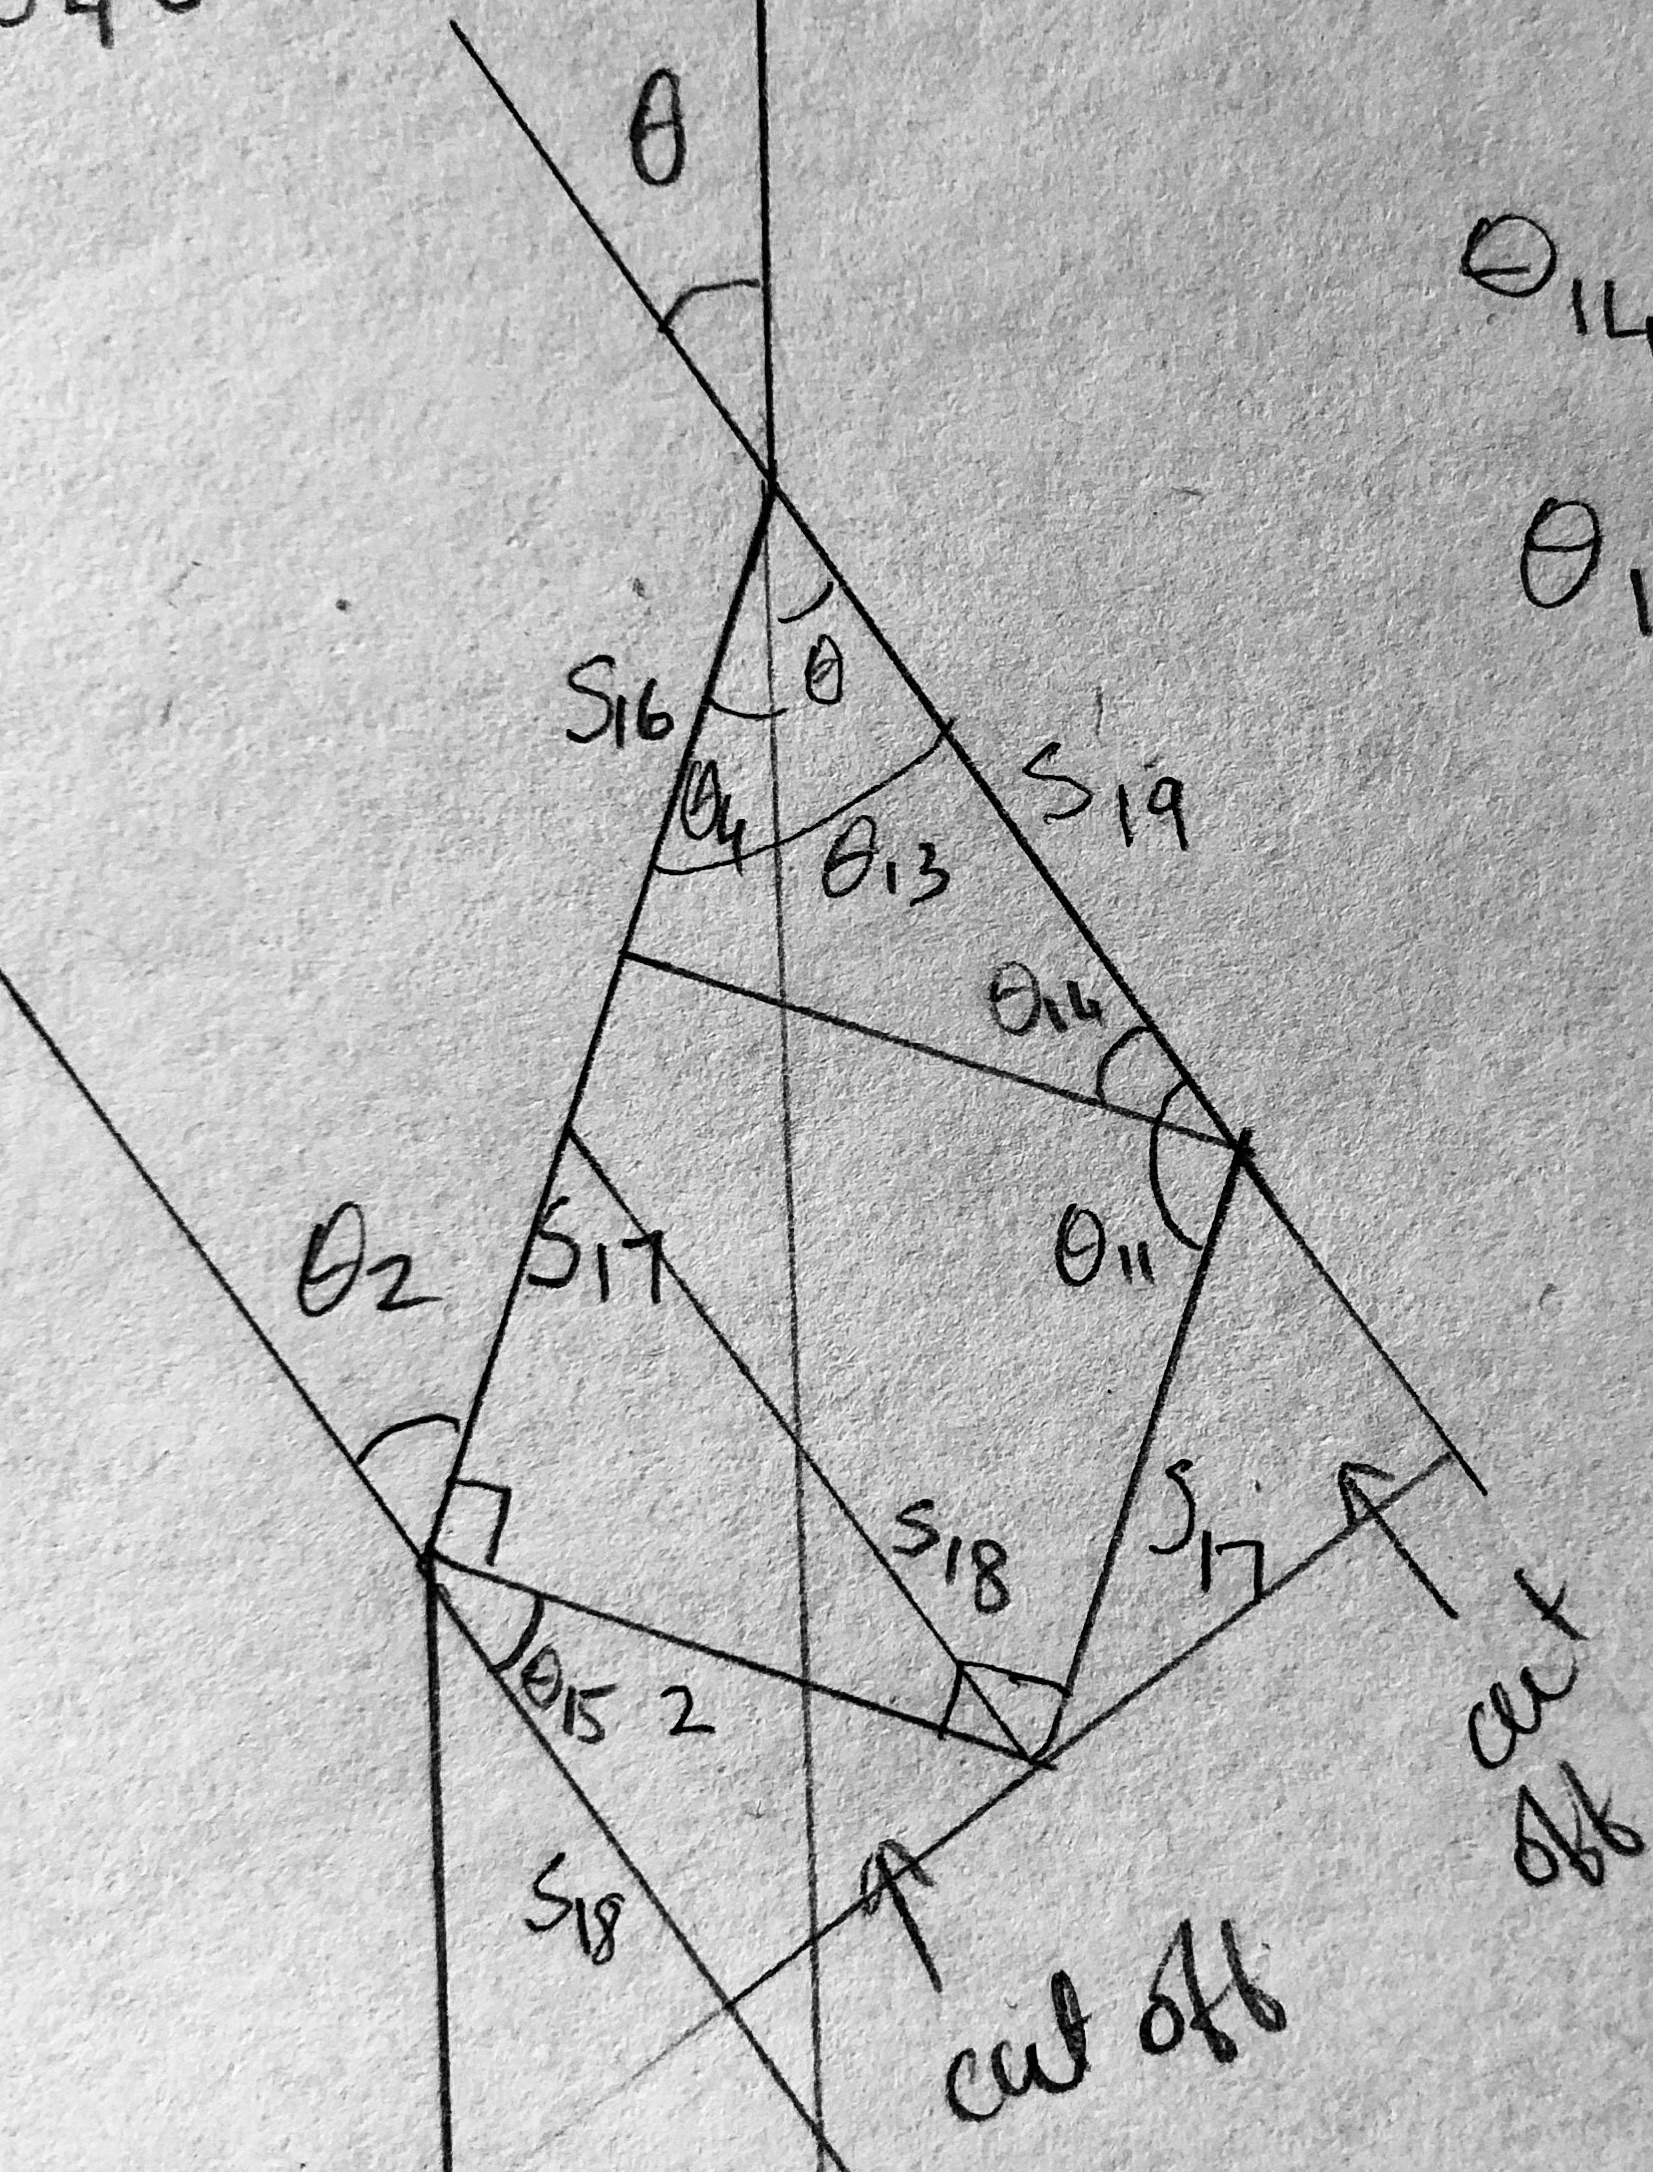
\includegraphics[width=0.4\textwidth]{images/strut_kp_tenon_detail}}
    \caption{Mortises for struts into KP (the one on the right is actually for tenons but usable for mortises)}
\end{figure}

\newpage


\subsection{Collar tie}


\begin{figure}[h]       
    \fbox{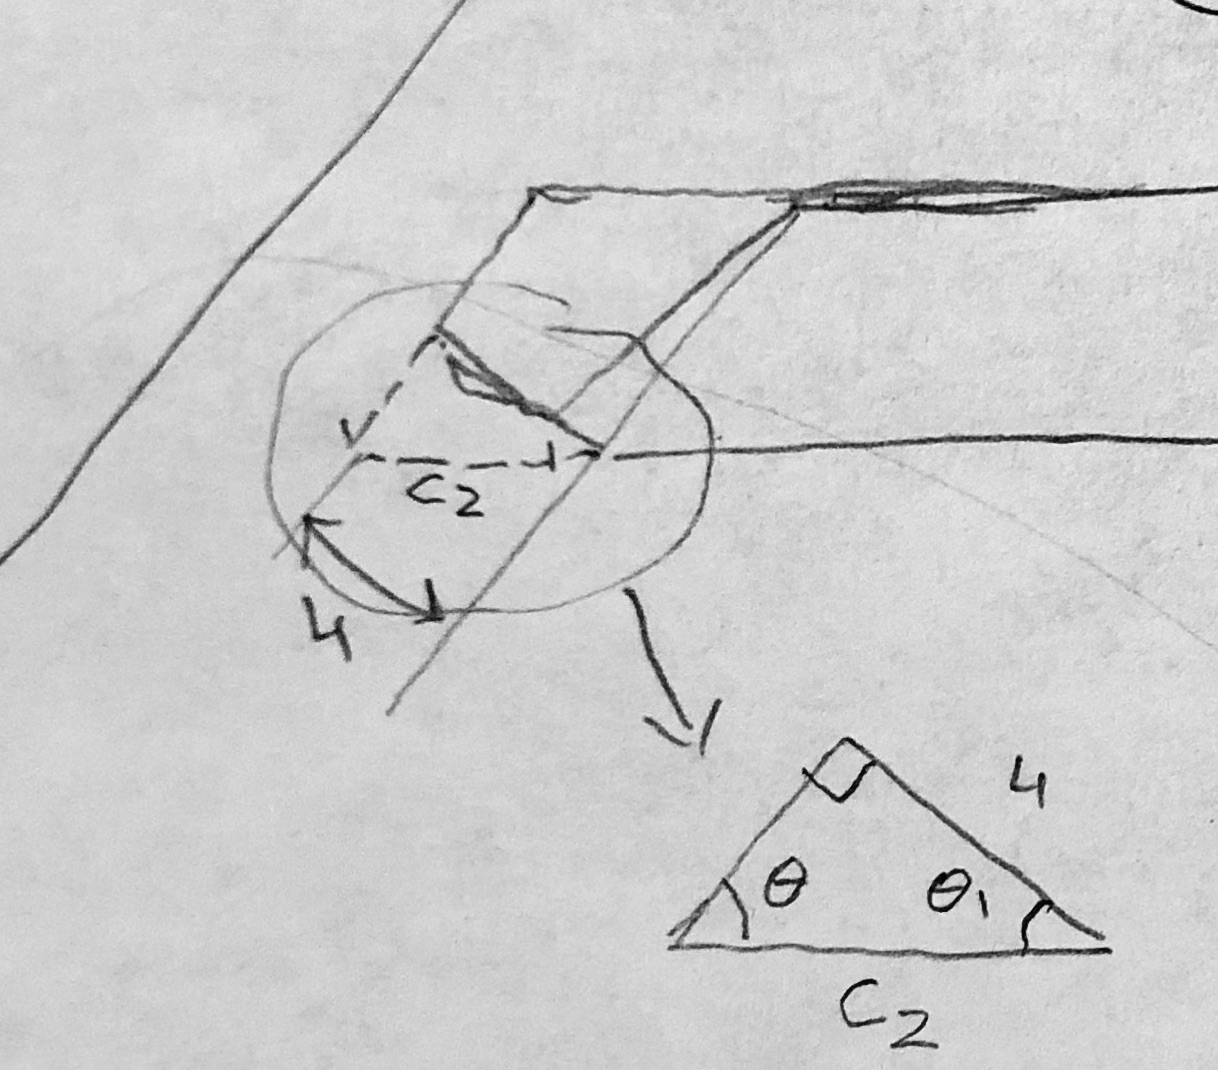
\includegraphics[width=0.39\textwidth]{images/ct_cut_plan}}   
    \hspace{30px}
    \fbox{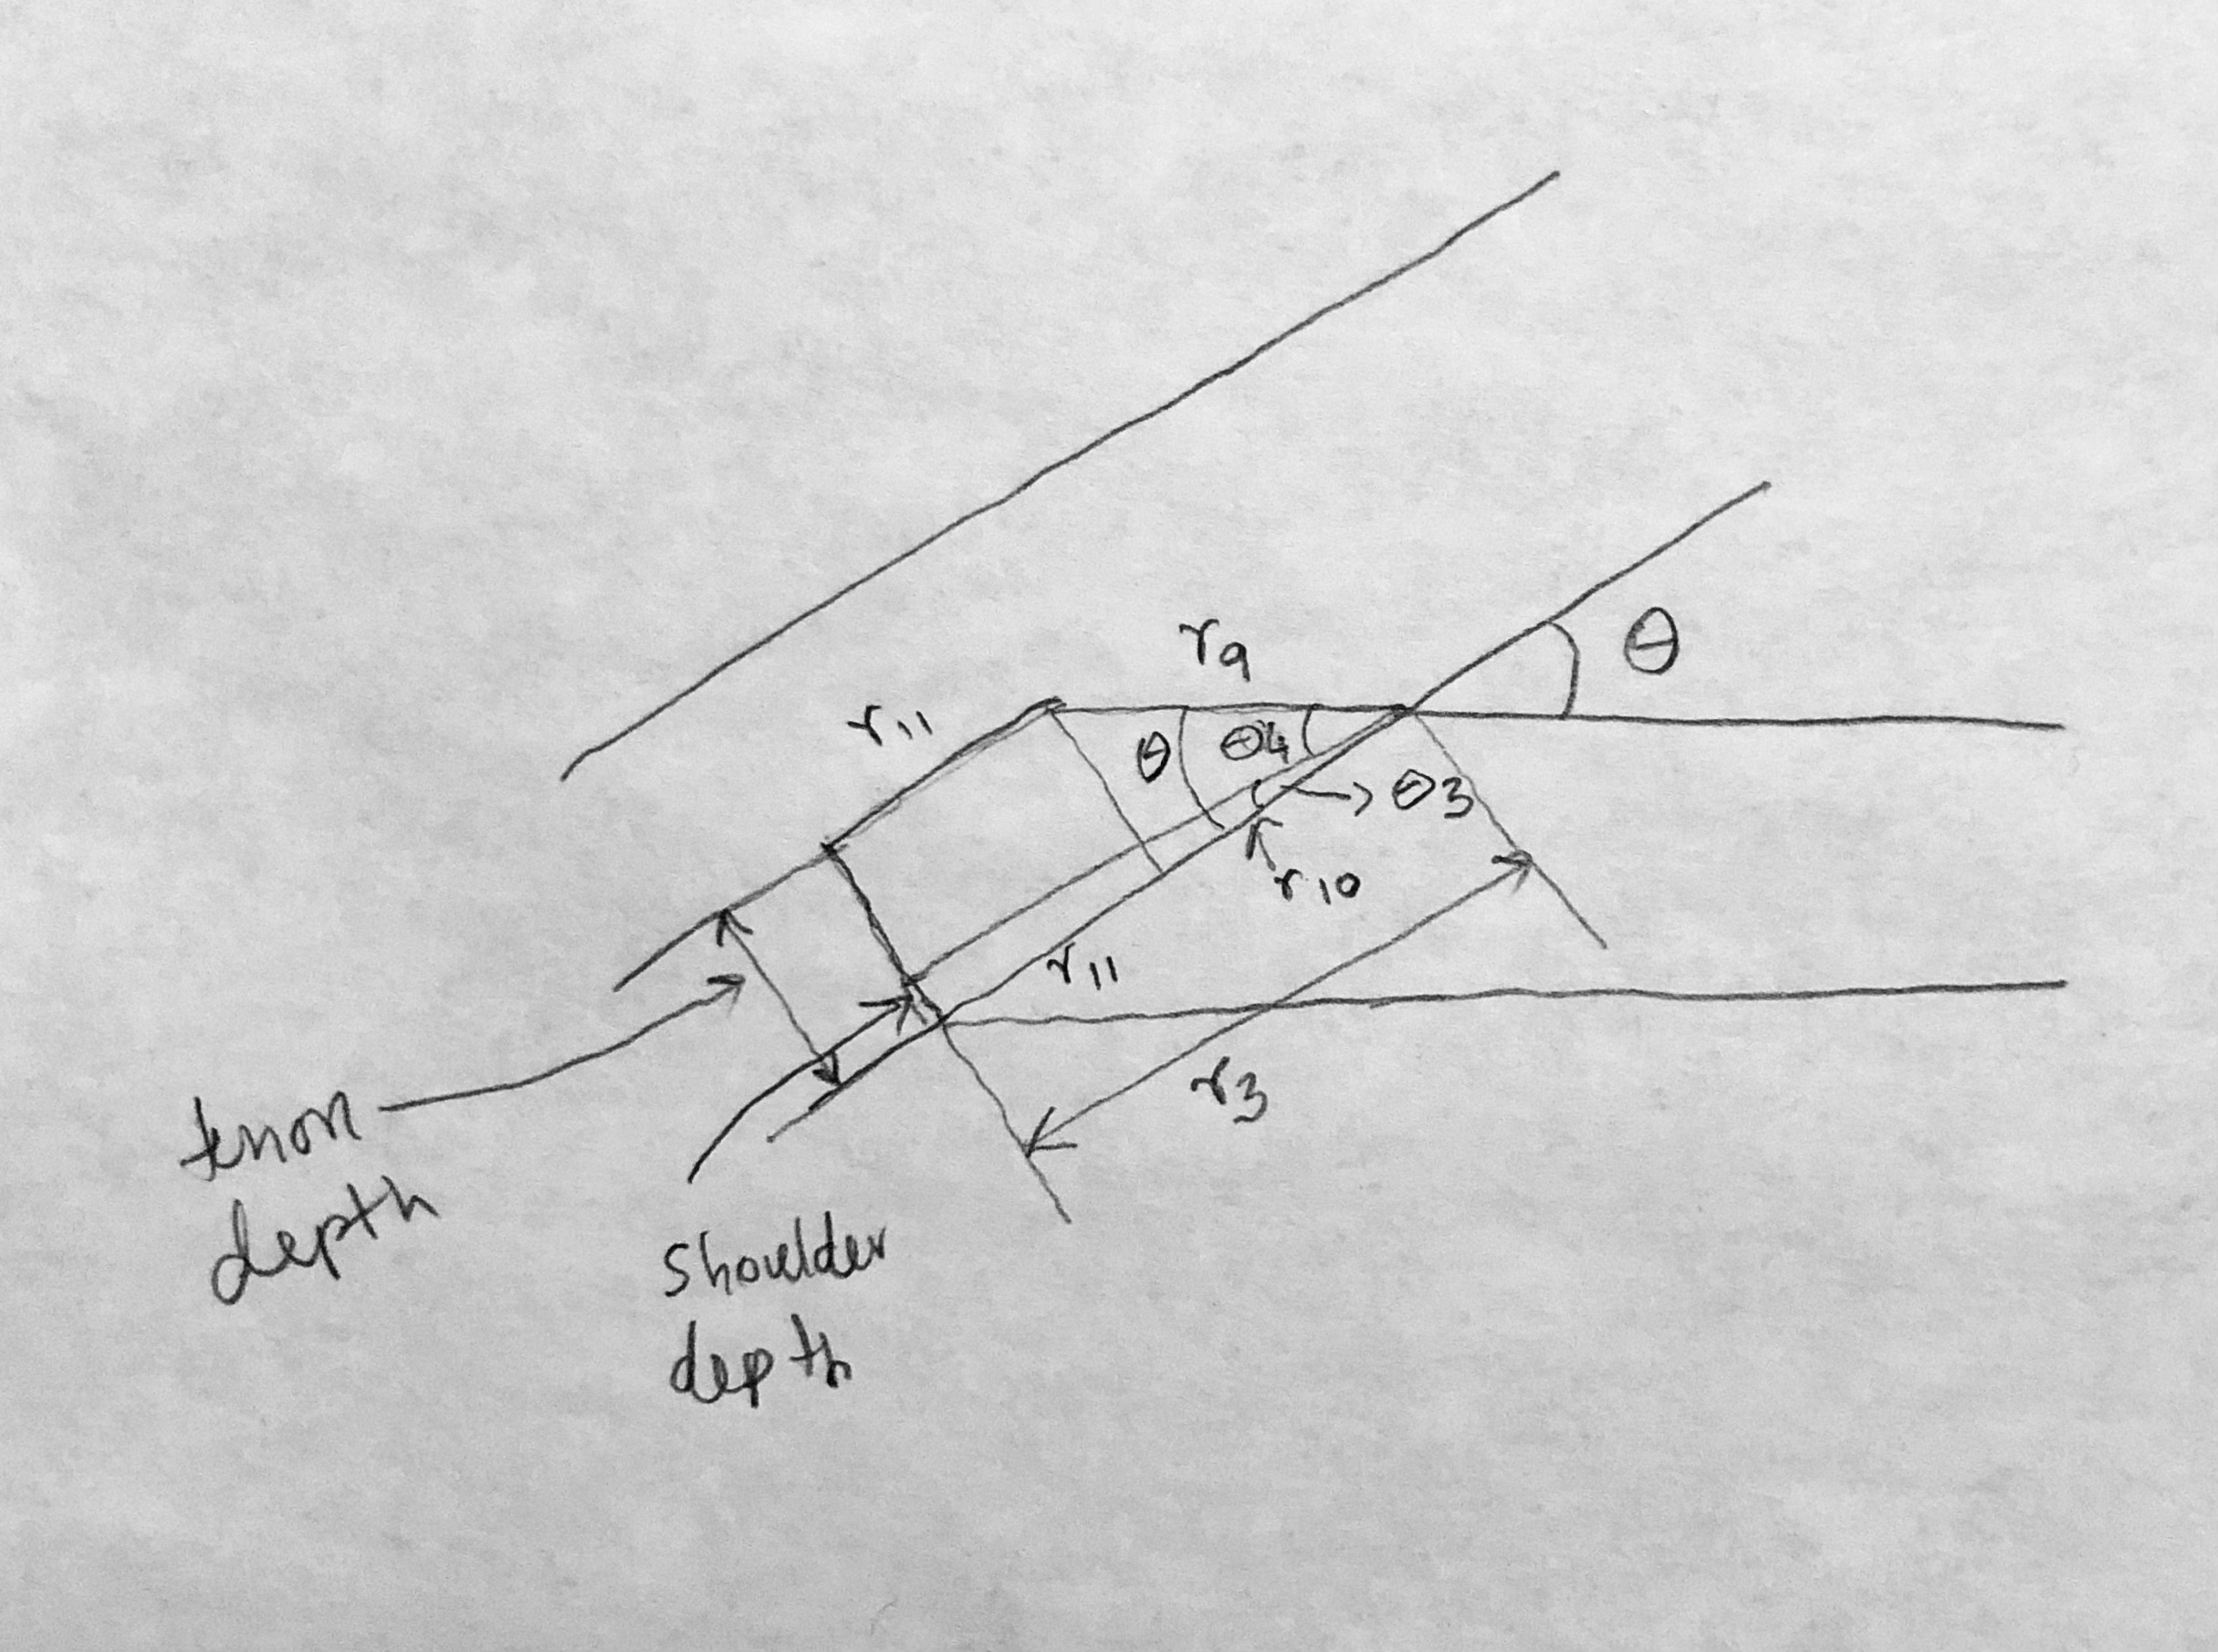
\includegraphics[width=0.46\textwidth]{images/collar_tie_tenons_into_rafters}}
    \caption{Tenons into rafters}
\end{figure}





\begin{enumerate}
  \item Cut beam to 6$\times$8 at 13' 11" 1/2 long. Note that $\text{CT length }= c_1\times 2 + 10 + c_2\times 2$. 
  \item Mark out $c_2$ = 0' 6" 1/4 at both ends.
  \item Mark out on the sides, shoulder depth = 1 and full tenon depth = 4.
  \item Mark $r_{11}$ = 0' 7" 11/16 and then $r_9$ = 0' 6" 1/4. 
  \item Connect line to shoulder and verify that $\theta_3$ = 4.6. 
  \item Cut off sections and create 2-inch thick tenons. 
  \item Mark out $c_1$ = 6' 0" 1/2 from both sides and verify that the middle section measures 10 inches.
  \item Cut through mortise at 2-in thick.
  % \item For KP tenons into collar tie see \Cref{kp-layout-and-cuts}, p. \pageref{kp-layout-and-cuts}. 
  \item Mark out $b_2$ = 1' 11" 5/32, $b_9$ = 0' 7" 13/16, and verify that distance between brace end to kp mortise beginning is 3' 5" 17/32. 
  \item Cut mortises for braces as shown. 
\end{enumerate}

\begin{figure}[h]
    \fbox{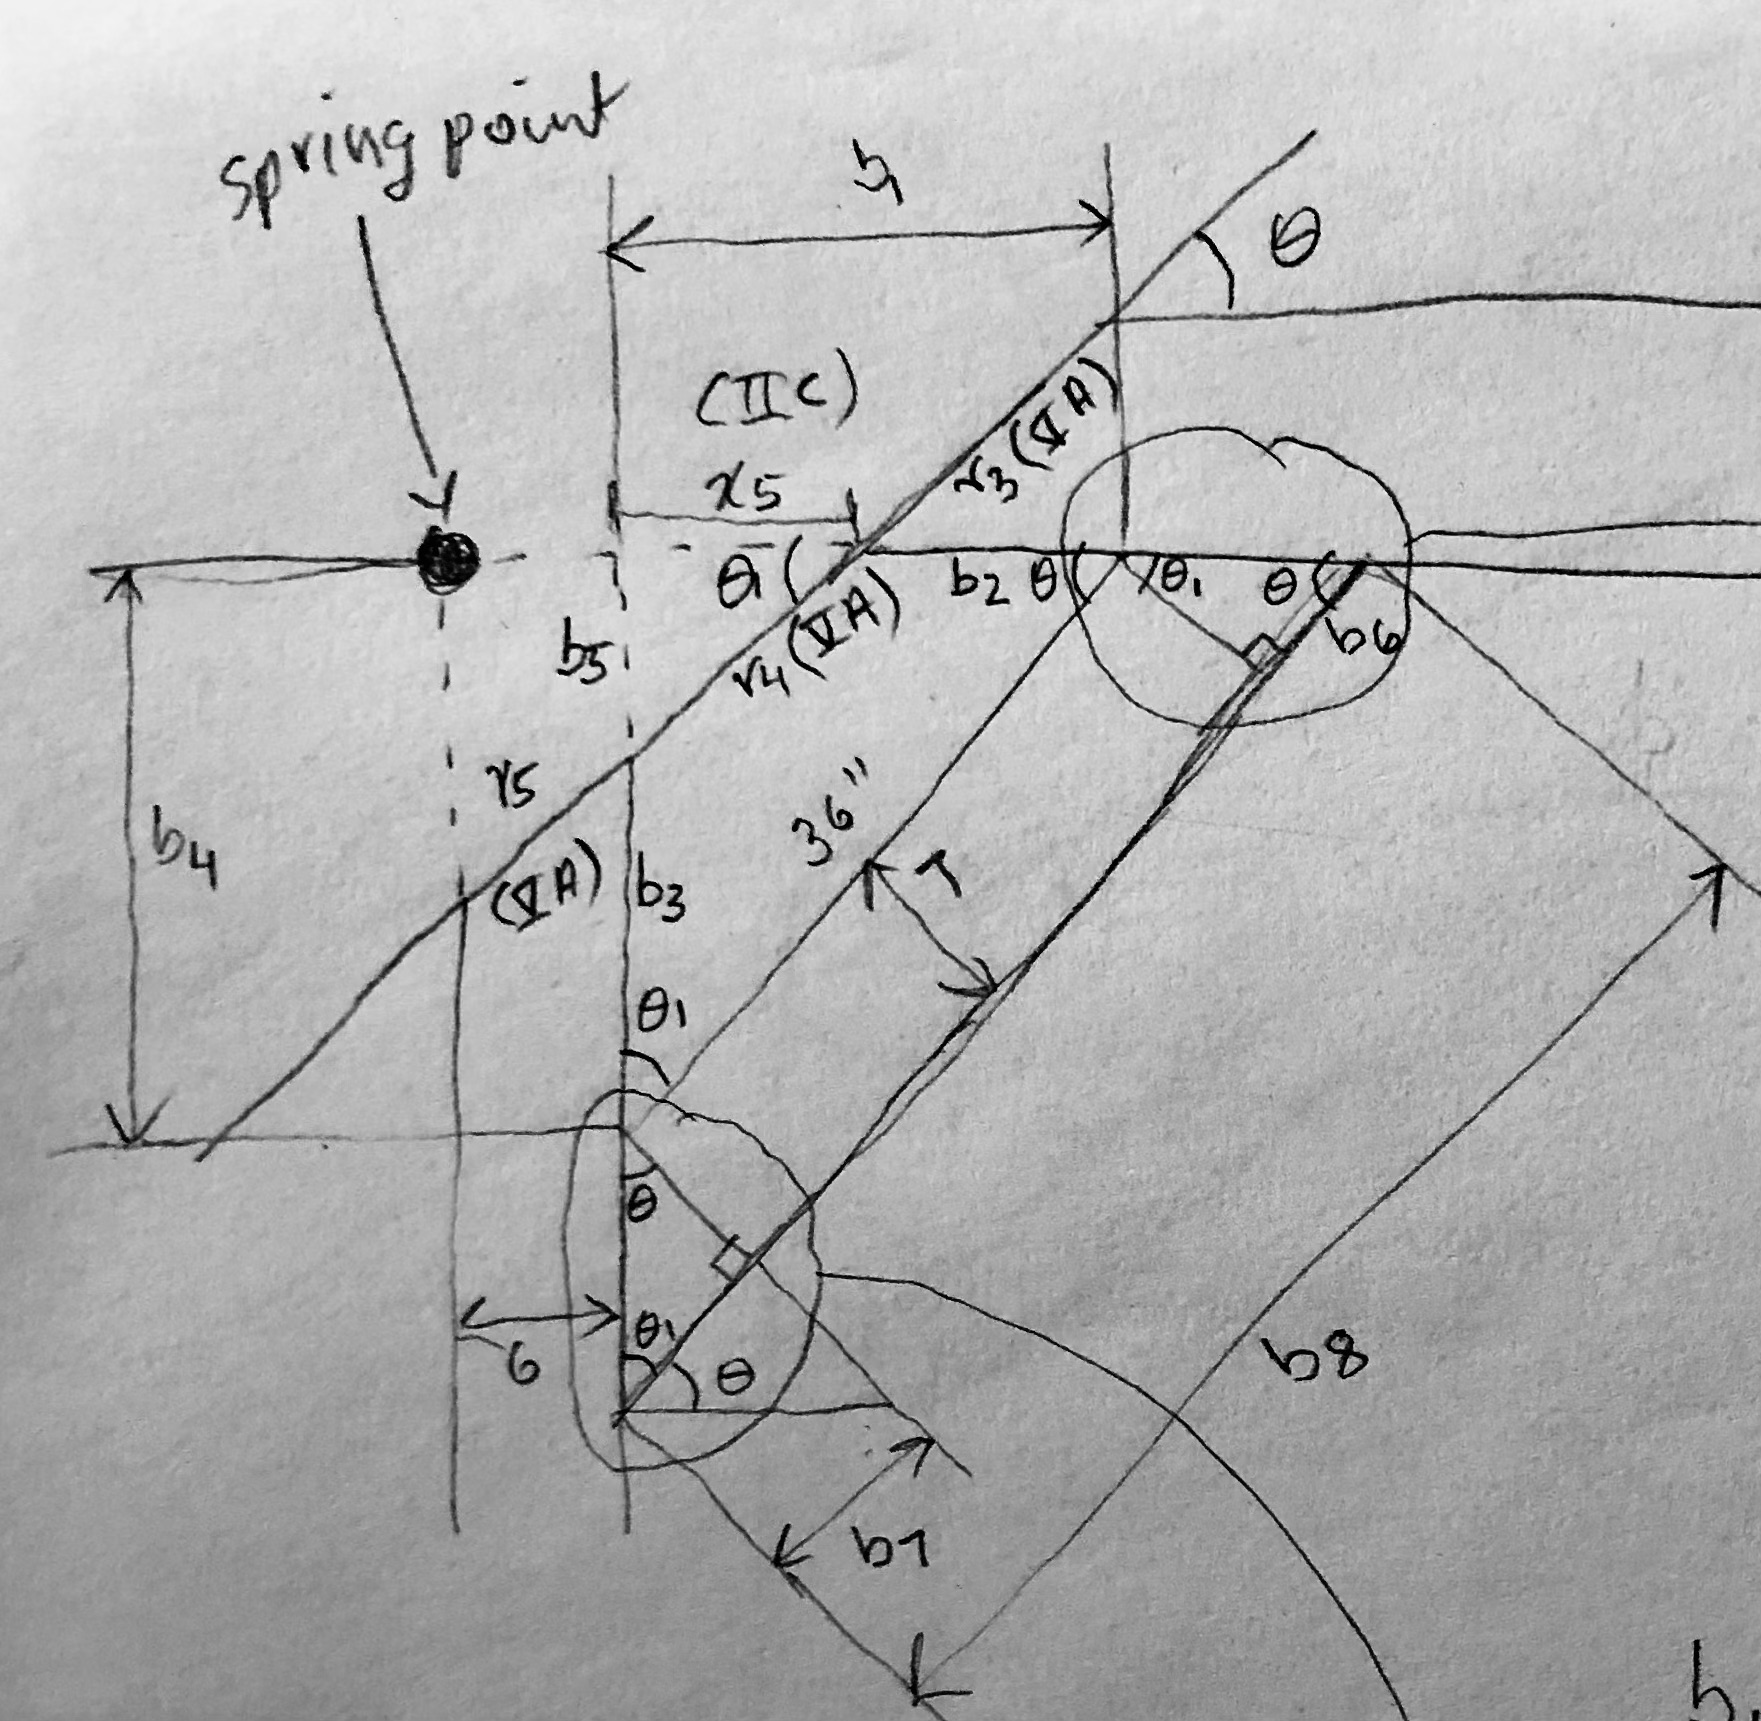
\includegraphics[width=0.4\textwidth]{images/braces_overall}}   
    \hspace{30px}
    \fbox{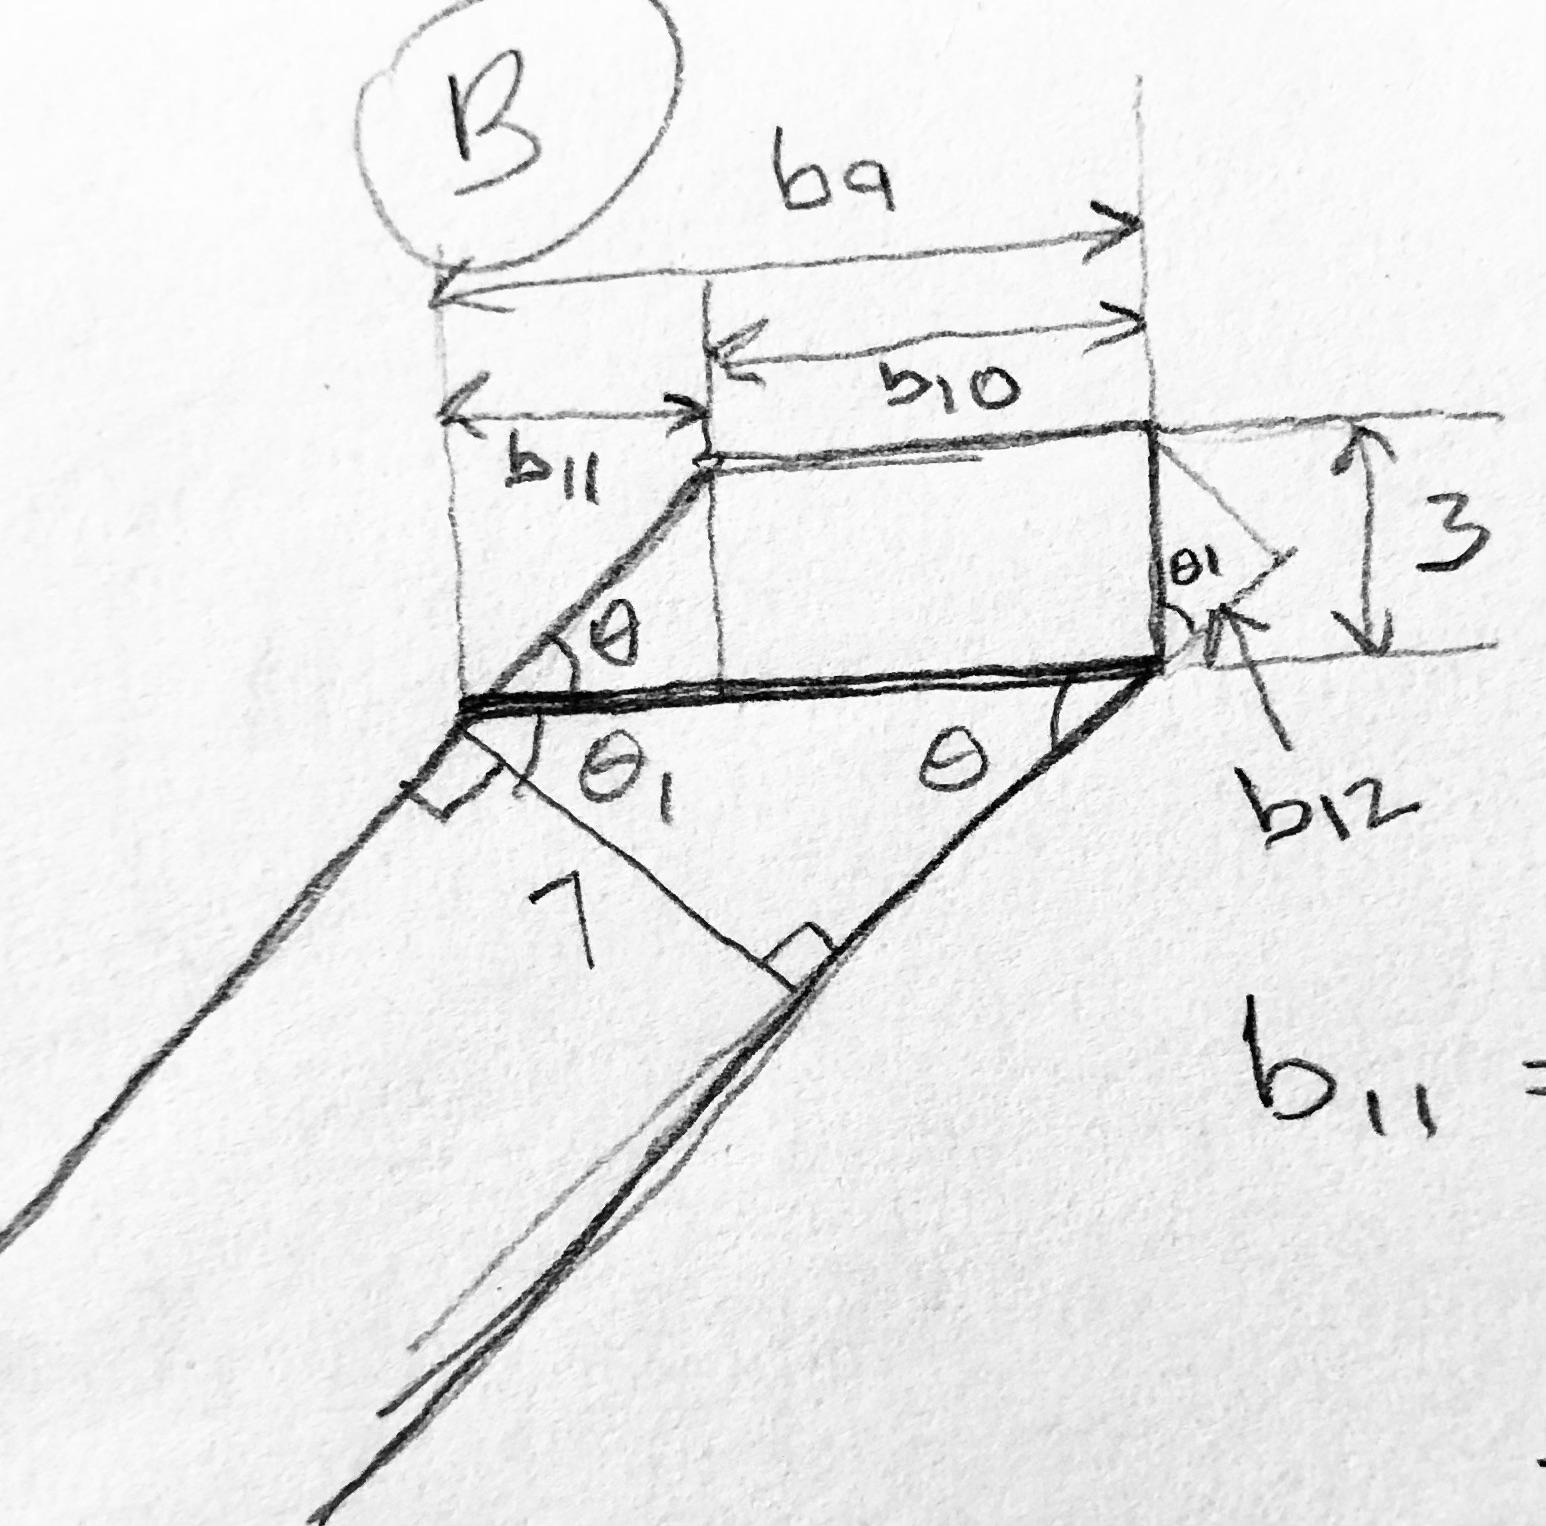
\includegraphics[width=0.4\textwidth]{images/braces_into_ct}}
    \caption{Mortises for knee braces}
\end{figure}

\newpage
\subsection{Struts}
\begin{figure}[h]
    \fbox{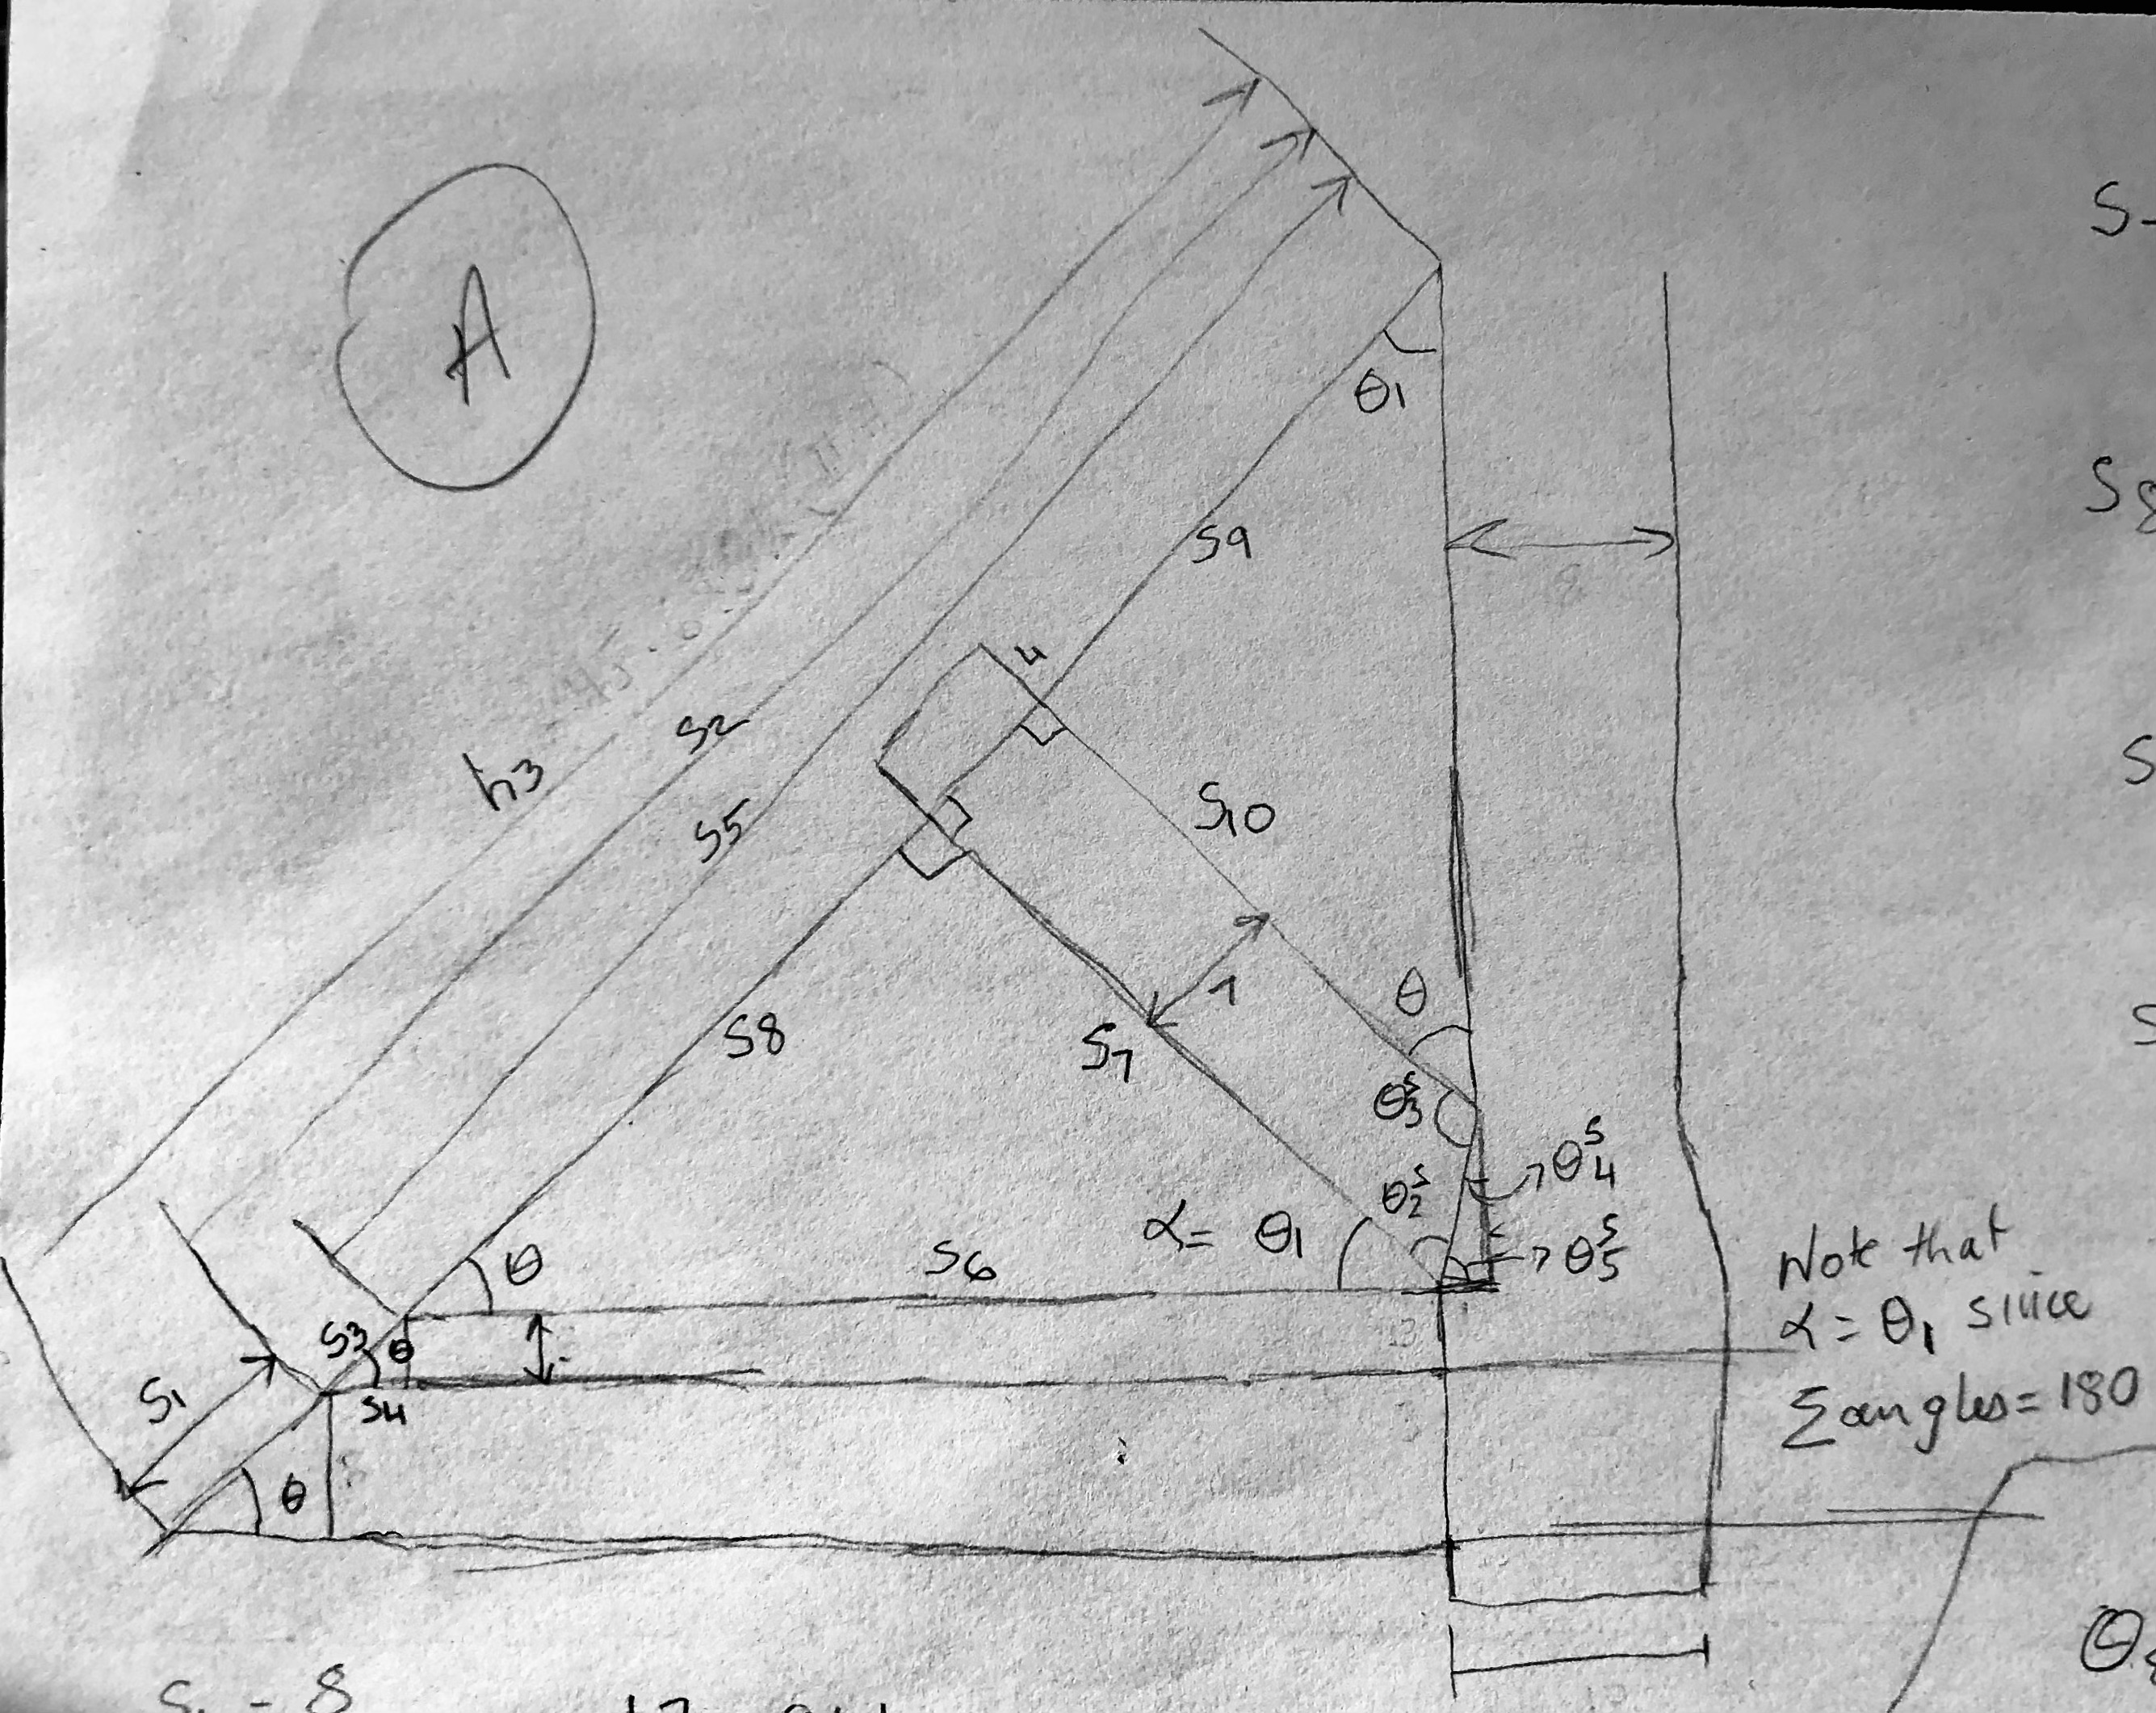
\includegraphics[width=0.57\textwidth]{images/strut_kp_overall}}   
    \hspace{10px}
    \fbox{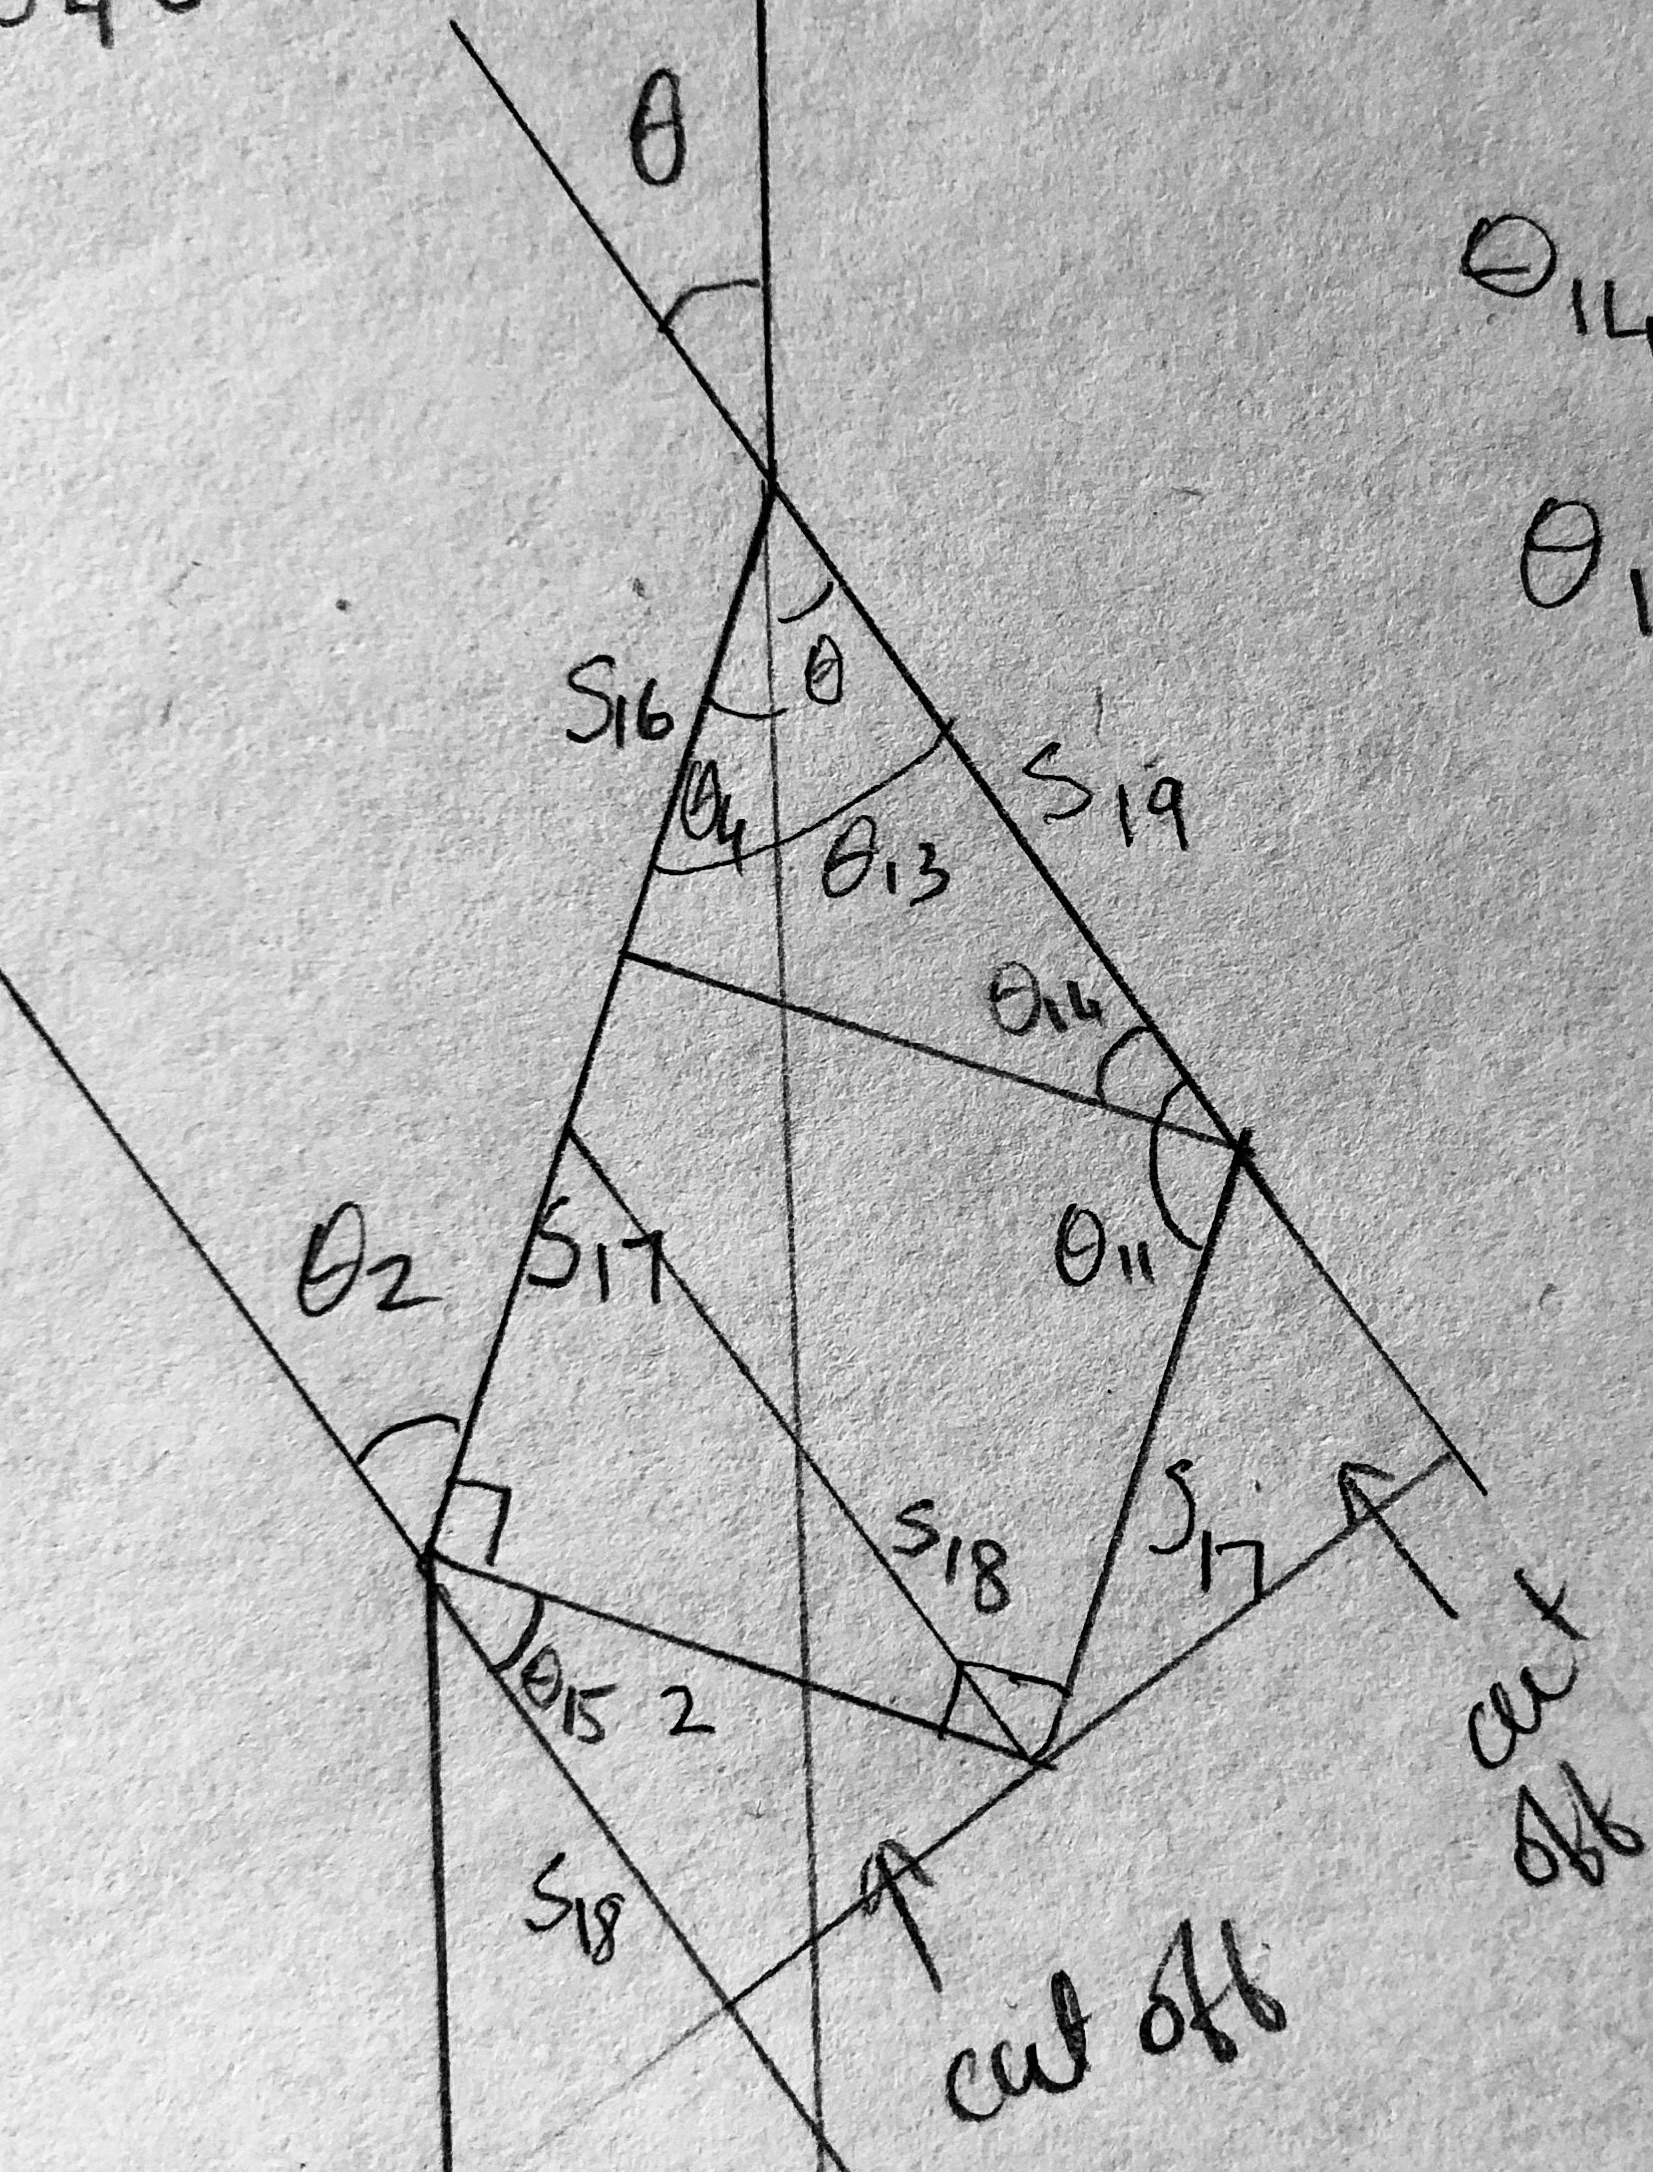
\includegraphics[width=0.35\textwidth]{images/strut_kp_tenon_detail}}
    \caption{Strut cuts}
\end{figure}

\begin{center}\fbox{There seems to be an extra $s_{18}$ in the diagram in the middle - not sure what that is.}\end{center}

\begin{enumerate}
  \item Strut length = strut tenon into rafter depth $+s_7 + s_{18} = $ 43.384 = \text{3' 7" 3/8}.
  \item At $s_{18}$, mark out $\theta_{15} = $ 44.8.
  \item At 2-in mark $90^\circ$ and measure $s_{17} = $ 0' 5" 1/4.
  \item Connect from $s_{17}$ end to other side of strut and verify $s_{19} = $0' 2" 11/16.
  \item Verify $\theta_{11} = $ 132 and $\theta_{13} = $ 48. 
  \item Draw tenon line, verify length is $s_{16} + s_{17}$ = 0' 7" 1/16.
  \item Cut off sections shown.
  \item Create tenons at 2 inches deep and 1.5 inches thick. 
  \item For strut tenons into rafter: tenon is 1.5-in thick, 5-in wide, and 4-in deep. 
\end{enumerate}




\newpage
\subsection{Braces}



\begin{figure}[h]
    \fbox{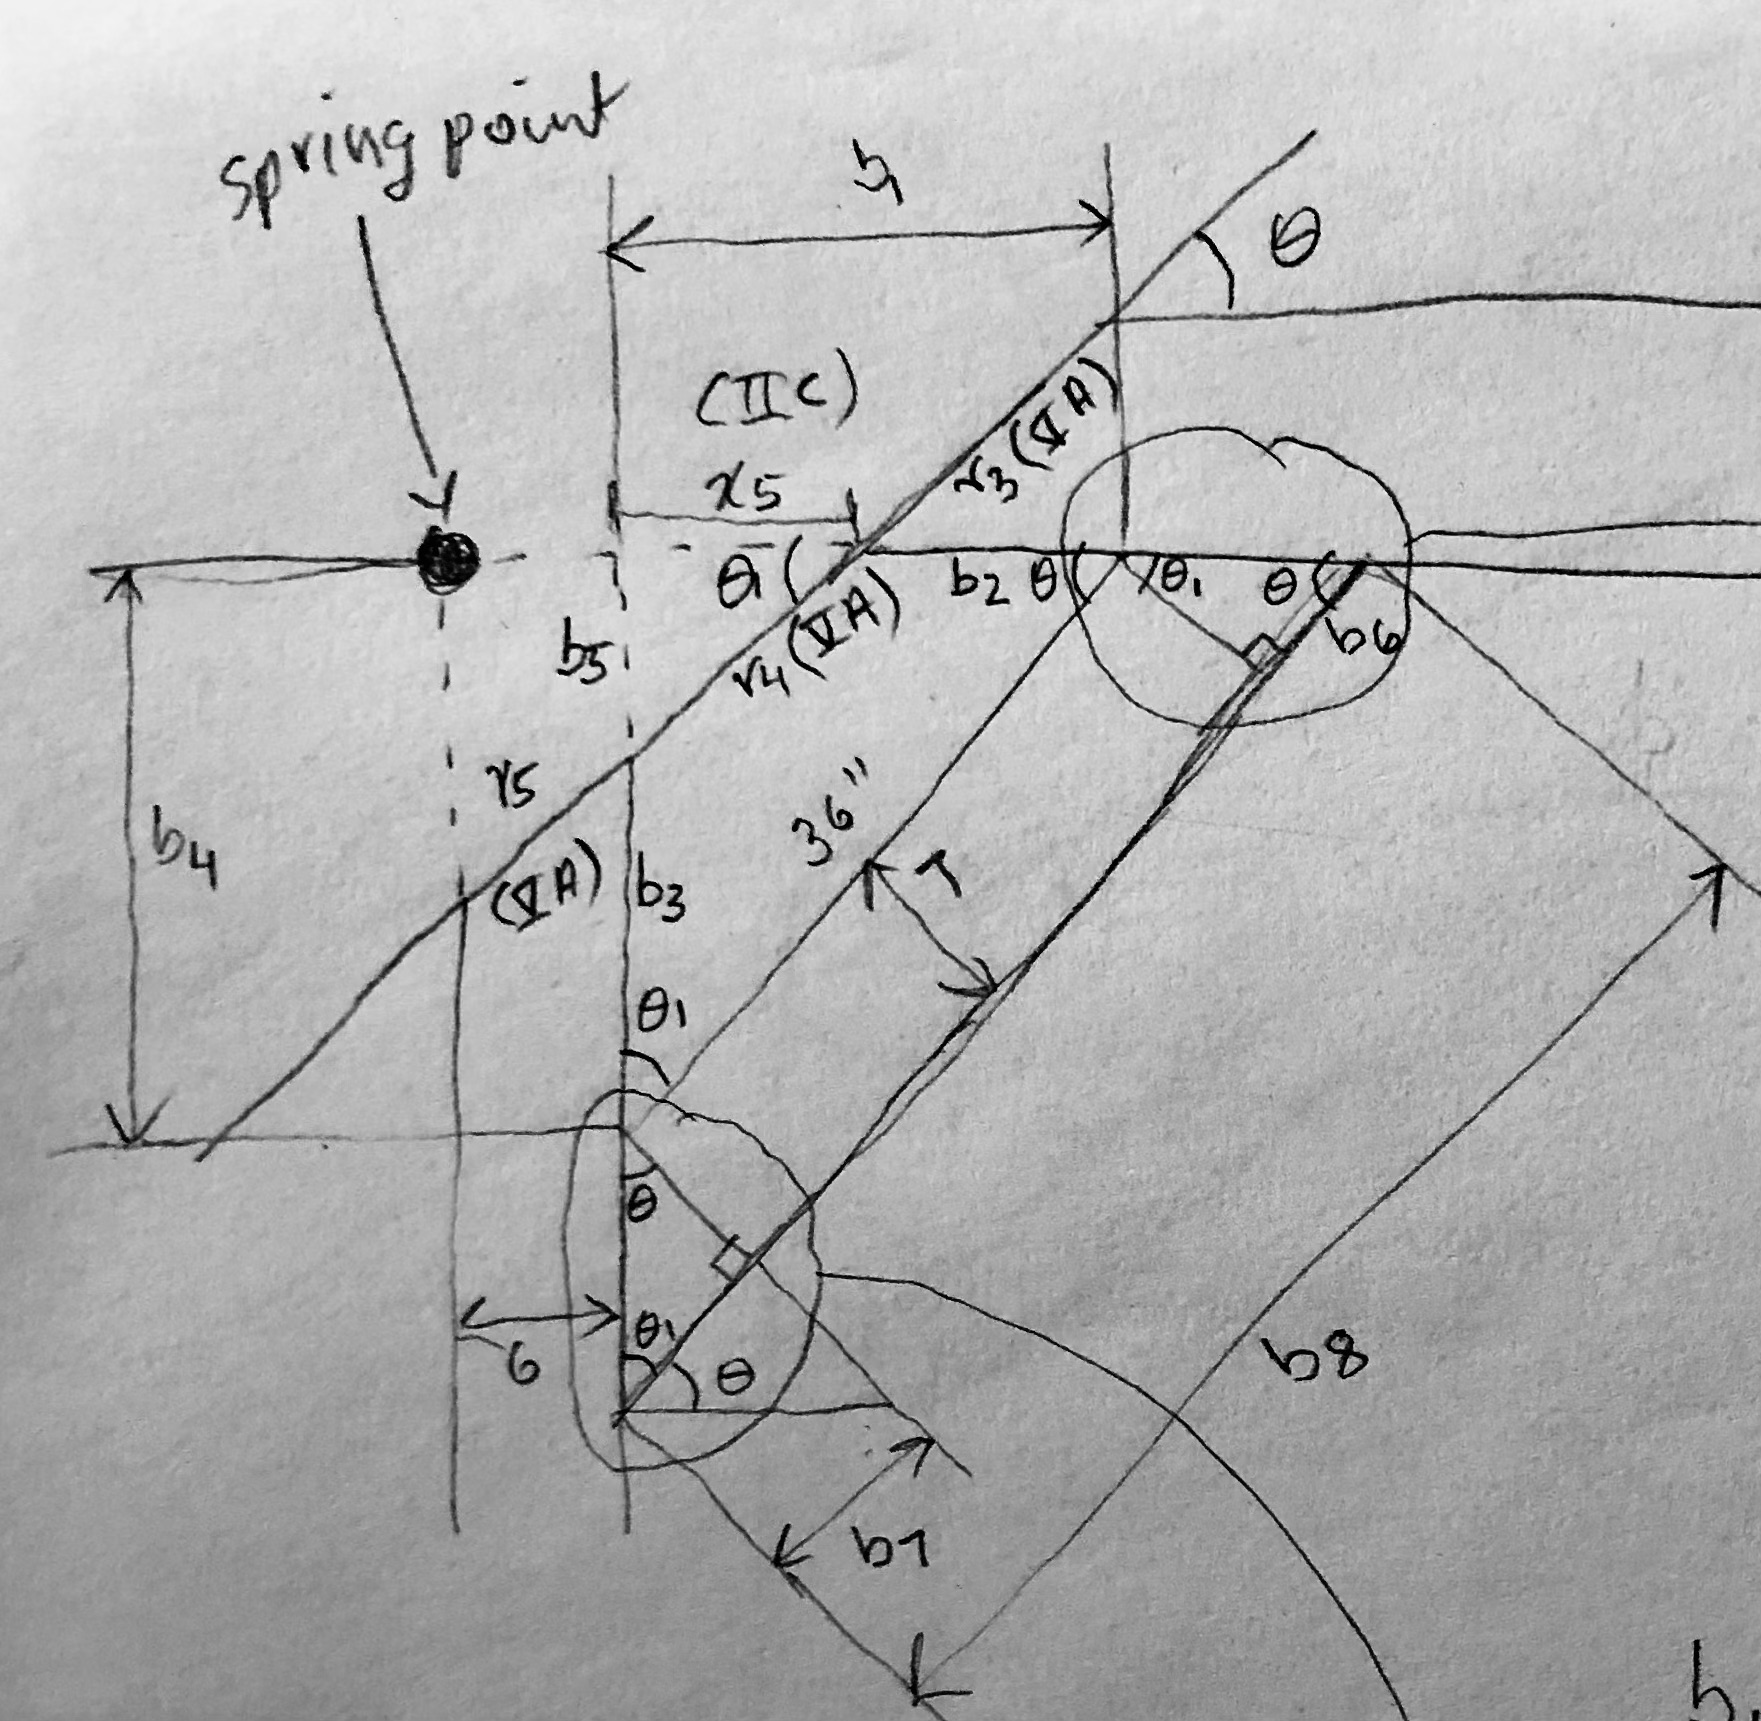
\includegraphics[width=0.25\textwidth]{images/braces_overall}}   
    \hspace{10px}
    \fbox{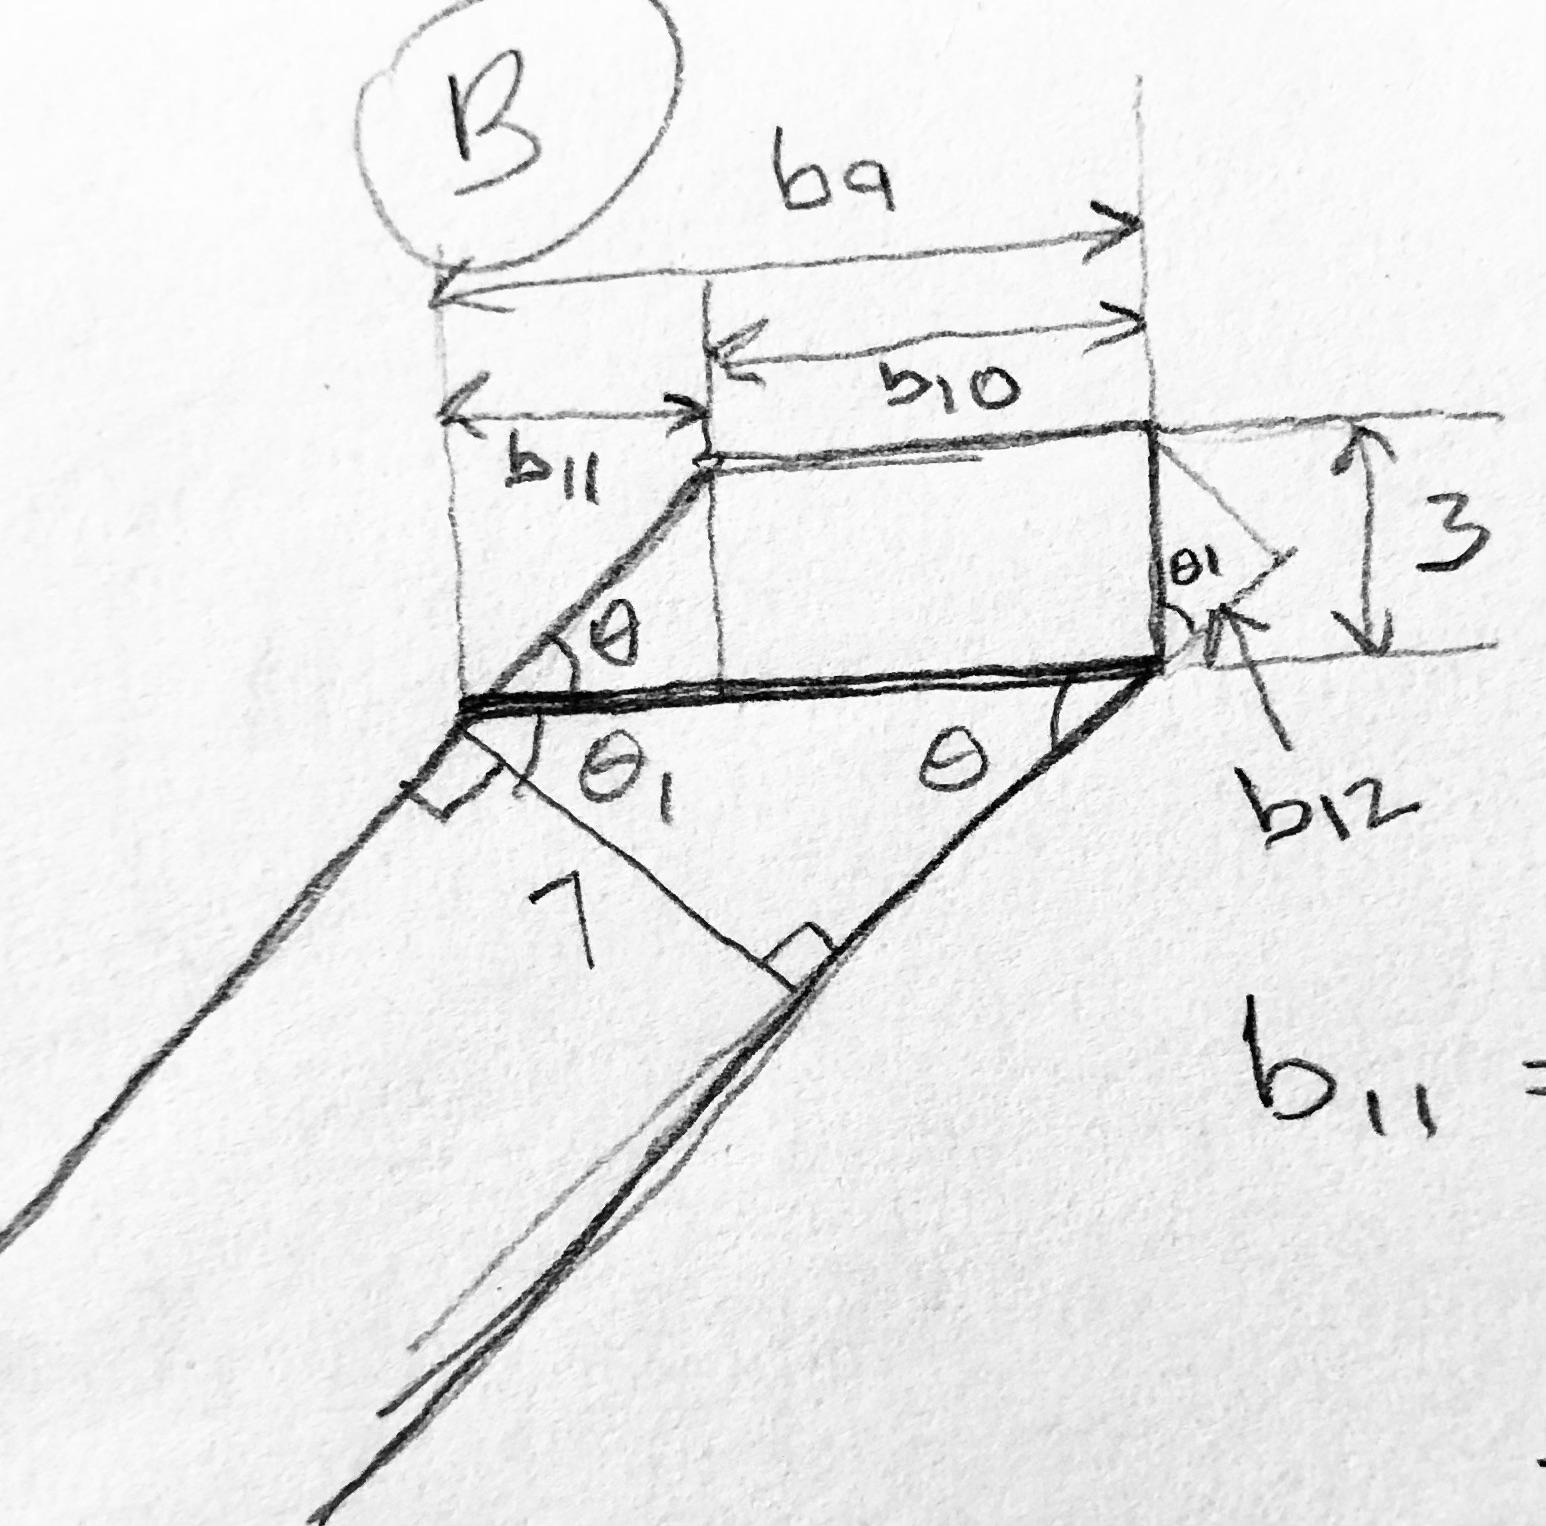
\includegraphics[width=0.25\textwidth]{images/braces_into_ct}}
    \hspace{10px}
    \fbox{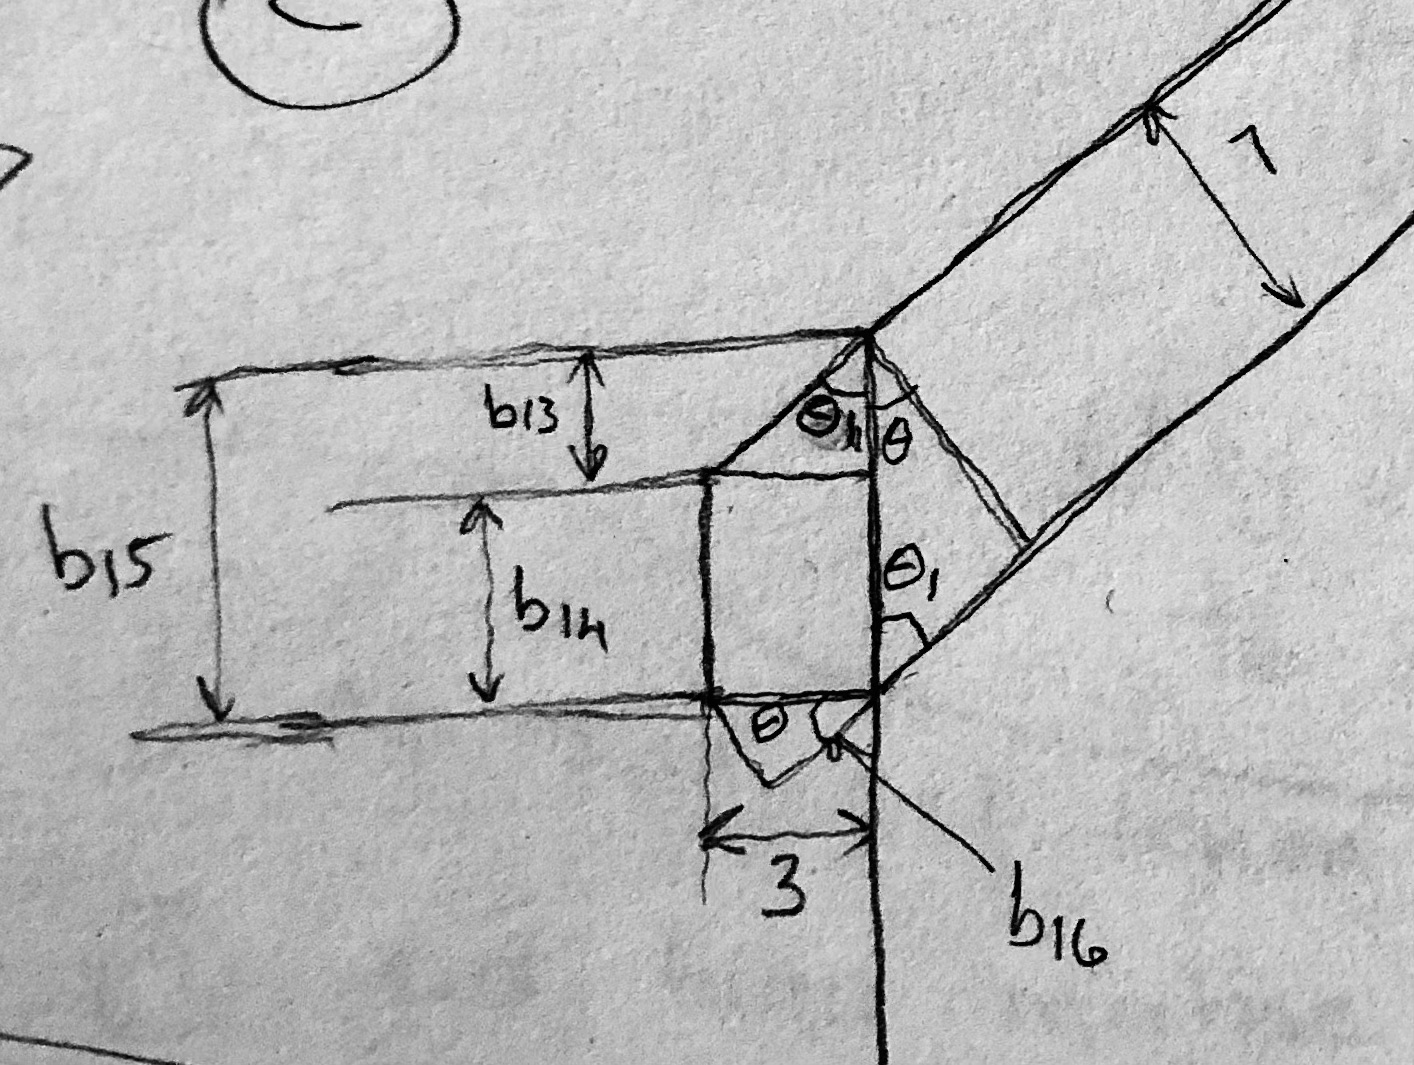
\includegraphics[width=0.33\textwidth]{images/braces_into_post}}
    \caption{Braces}
\end{figure}

\begin{enumerate}
  \item Brace length = $b_8 + b_{12} + b_{16} = $ 4' 2" 13/32. 
  \item There are no shoulders; just cut according to diagrams/calculations above and verify the important $b_{X}$ variables. 
\end{enumerate}


\newpage



\section{Measurements for scale diagram}
\begin{multicols}{2}
Angles (static):
\begin{itemize}
  \item $\theta$ = 39.8
  \item $\theta_1$ = 50.2
\end{itemize}
\columnbreak
Angles (dynamic):
\begin{itemize}
  \item $\theta$ = 39.8
  \item $\theta_1$ = 50.2
\end{itemize}
\end{multicols}

Scale for lengths is 1 cm = 10 inches. 

\begin{multicols}{2}
Lengths (static; version of 6-inch posts, and fat struts/braces):
\begin{itemize}
  \item $b_2$ = 2.12
  \item $b_3$ = 1.66
  \item $b_8$ = 5.02
  \item $h_1$ = 0.94
  \item $h_2$ = 1.25
  \item $h_4$ = 12.94
  \item $k_3$ = 1.04
  \item $k_{17}$ = 4.02
  \item $s_{13}$ = 1.01
  \item $x_1$ = 8
  \item $x_2$ = 7.35
  \item $x_3$ = 0.65
  \item $x_6$ = 0.54
  \item $x_8$ = 3.12
  \item base to spring line = 9.72
  \item brace width = 0.7
  \item collar tie height = 0.8
  \item ct/rafter shoulder = 0.1
  \item kp part = 0.45
  \item KP width at bottom = 1
  \item KP width at top = 0.8
  \item kp/rafter shoulder = 0.1
  \item post width = 0.6
  \item post/rafter shoulder = 0.1
  \item purlin height = 0.7
  \item purlin pocket depth = 0.1
  \item rafter height = 0.8
  \item ridge ht = 0.66
  \item ridge straight part = 0.33
  \item straight part KP below flare = 0.3
  \item structure height = 18
  \item structure width = 18
  \item strut width = 0.7
  \item through tenon length = 0.2
\end{itemize}
\columnbreak
Lengths (dynamic):
\begin{itemize}
  \item $b_2$ = 2.32
  \item $b_3$ = 1.86
  \item $b_8$ = 4.62
  \item $h_1$ = 0.94
  \item $h_2$ = 1.25
  \item $h_4$ = 11.72
  \item $k_3$ = 1.04
  \item $k_{17}$ = 4.33
  \item $s_{13}$ = 0.7
  \item $x_1$ = 7.8
  \item $x_2$ = 7.35
  \item $x_3$ = 0.45
  \item $x_6$ = 0.37
  \item $x_8$ = 3.12
  \item base to spring line = 9.72
  \item brace width = 0.5
  \item collar tie height = 0.8
  \item ct/rafter shoulder = 0.1
  \item kp part = 0.45
  \item KP width at bottom = 1
  \item KP width at top = 0.8
  \item kp/rafter shoulder = 0.1
  \item post width = 0.8
  \item post/rafter shoulder = 0.1
  \item purlin height = 0.7
  \item purlin pocket depth = 0.1
  \item rafter height = 0.8
  \item ridge ht = 0.66
  \item ridge straight part = 0.33
  \item straight part KP below flare = 0.3
  \item structure height = 18
  \item structure width = 18
  \item strut width = 0.5
  \item through tenon length = 0.2
\end{itemize}
\end{multicols}

\newpage





\end{document}
